\ifdefined\pdfadjustspacing\pdfadjustspacing=0\fi
\newpage
\chapter{\MakeUppercase{Cơ sở lý thuyết}} 
\section{Giới thiệu chung về CCC}
Car Connectivity Consortium (CCC) là một tổ chức liên ngành toàn cầu với sự tham gia của các nhà sản xuất ô tô hàng đầu (BMW, Audi, Ford,...) và các tập đoàn công nghệ lớn (Apple, Samsung, Google,...). Mục tiêu cốt lõi của CCC là phát triển các tiêu chuẩn công nghệ toàn cầu cho các giải pháp kết nối giữa điện thoại thông minh và phương tiện giao thông.

Trong bối cảnh các hệ thống Smart Key truyền thống đối mặt với nhiều rủi ro bảo mật (đặc biệt là Relay Attack), CCC đã ban hành tiêu chuẩn \textbf{Digital Key Release 3.0} \cite{ccc_digikey3}. Đây là một bước ngoặt công nghệ khi lần đầu tiên chuẩn hóa việc kết hợp ba công nghệ không dây: NFC, BLE và UWB vào một kiến trúc bảo mật thống nhất, cho phép người dùng mở khóa và khởi động xe bằng thiết bị di động một cách an toàn mà không cần lấy điện thoại ra khỏi túi (Passive Keyless Entry).

\subsection{Kiến trúc tổng thể của CCC Digital Key Release 3.0}
Kiến trúc Digital Key của CCC được xây dựng dựa trên nguyên lý xác thực đa lớp (Multi-layer Authentication) và đo lường khoảng cách an toàn (Secure Ranging). Kiến trúc này phân công nhiệm vụ chuyên biệt cho từng công nghệ vô tuyến:

\begin{enumerate}
    \item \textbf{NFC (Near Field Communication):} 
    Đóng vai trò là phương thức giao tiếp dự phòng (Fallback) và khởi tạo (Provisioning). Trong trường hợp điện thoại hết pin, chuẩn CCC quy định thiết bị vẫn phải duy trì năng lượng tối thiểu cho chip NFC (chế độ Host Card Emulation) để người dùng có thể chạm thiết bị vào tay nắm cửa và mở xe.
    
    \item \textbf{BLE (Bluetooth Low Energy):} 
    Hoạt động như một kênh truyền thông tin cậy (Secure Channel) ở khoảng cách xa. Khi người dùng tiến lại gần phương tiện, BLE sẽ thức giấc, thực hiện trao đổi khóa mật mã (Key Exchange) và xác thực danh tính hai chiều (Mutual Authentication) trước khi hệ thống UWB được kích hoạt.
    
    \item \textbf{UWB (Ultra-Wideband):} 
    Thành phần cốt lõi của Release 3.0 nhằm chống lại Relay Attack. Sau khi BLE xác thực thành công, UWB thực hiện các phép đo thời gian bay (Time-of-Flight) kết hợp mã hóa (STS - Scrambled Timestamp Sequence) để xác minh chính xác vị trí vật lý của thiết bị. Xe chỉ mở cửa khi thiết bị nằm trong vùng an toàn (Secure Zone) quy định (ví dụ: cách cửa xe dưới 2 mét).
\end{enumerate}

\begin{figure}[H]
    \centering
    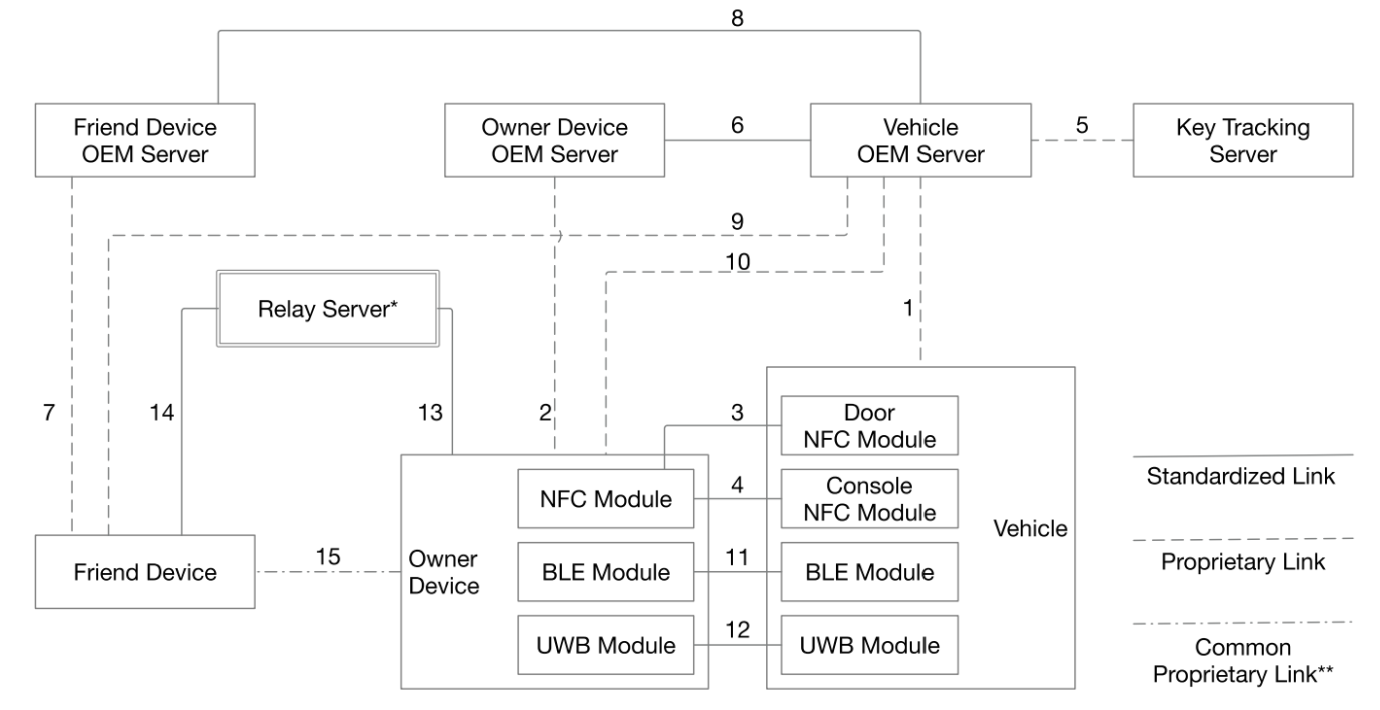
\includegraphics[width=0.8\textwidth]{image/section3/ccc_architecture.png} 
    \caption[Kiến trúc giao tiếp NFC, BLE và UWB theo chuẩn CCC 3.0]{Kiến trúc giao tiếp NFC, BLE và UWB theo chuẩn CCC 3.0 (\textbf{Nguồn:} \href{https://www.researchgate.net/publication/396275938_Mitigating_Relay_Attacks_in_Vehicle_Access_Systems_Using_BLE_and_UWB}{researchgate.net})}
    \label{fig:ccc_architecture}
\end{figure}

\subsection{Cơ chế chuyển trạng thái trong kiến trúc CCC}
Để đảm bảo luồng hoạt động chặt chẽ, chuẩn CCC định nghĩa các pha giao dịch mật mã như sau:
\begin{itemize}
    \item \textbf{Standard Transaction (Giao dịch tiêu chuẩn):} Là quá trình xác thực đầy đủ, bao gồm việc trao đổi chứng chỉ (Certificates) và khóa công khai (Public Keys) thông qua đường cong Elliptic (ECC). Pha này thường diễn ra ở lần kết nối đầu tiên hoặc khi cần thiết lập lại độ tin cậy.
    \item \textbf{Fast Transaction (Giao dịch nhanh):} Được tối ưu hóa cho các lần kết nối tiếp theo. Giao dịch này bỏ qua bước trao đổi chứng chỉ nặng nề, sử dụng lại các tham số đã được thỏa thuận trước đó để tăng tốc độ phản hồi khi người dùng bước lại gần xe, đảm bảo trải nghiệm liền mạch (Seamless experience).
\end{itemize}

Việc đề tài lấy chuẩn CCC Digital Key Release 3.0 làm kim chỉ nam thiết kế đòi hỏi hệ thống phải nắm vững và làm chủ đồng thời ba nhóm lý thuyết lõi: Công nghệ truyền thông vô tuyến, Mật mã học ứng dụng, và Kiến trúc vi điều khiển. Các nền tảng lý thuyết này sẽ được trình bày chi tiết trong các mục tiếp theo.

\section{Công nghệ truyền thông không dây}

Hệ thống Smart Car Access Control sử dụng ba công nghệ truyền thông không dây chính: NFC (Near Field Communication), BLE (Bluetooth Low Energy), và UWB (Ultra-Wideband). Mỗi công nghệ có đặc điểm riêng về phạm vi hoạt động, tốc độ truyền dữ liệu, công suất tiêu thụ và use cases phù hợp. Phần này trình bày chi tiết nguyên lý hoạt động, kiến trúc giao thức và ứng dụng của từng công nghệ.

\subsection{Near Field Communication - NFC}

\subsubsection{Giới thiệu và đặc điểm kỹ thuật} Near Field Communication (NFC) là công nghệ truyền thông không dây tầm ngắn hoạt động ở tần số \textbf{13.56 MHz} thuộc băng tần ISM (Industrial, Scientific and Medical) \cite{coskun2013professional}. NFC được phát triển dựa trên công nghệ RFID (Radio-Frequency Identification) và được chuẩn hóa bởi tổ chức ISO/IEC theo các tiêu chuẩn ISO/IEC 14443 và ISO/IEC 18092 \cite{iso14443}.

\begin{figure}[H]
    \centering
    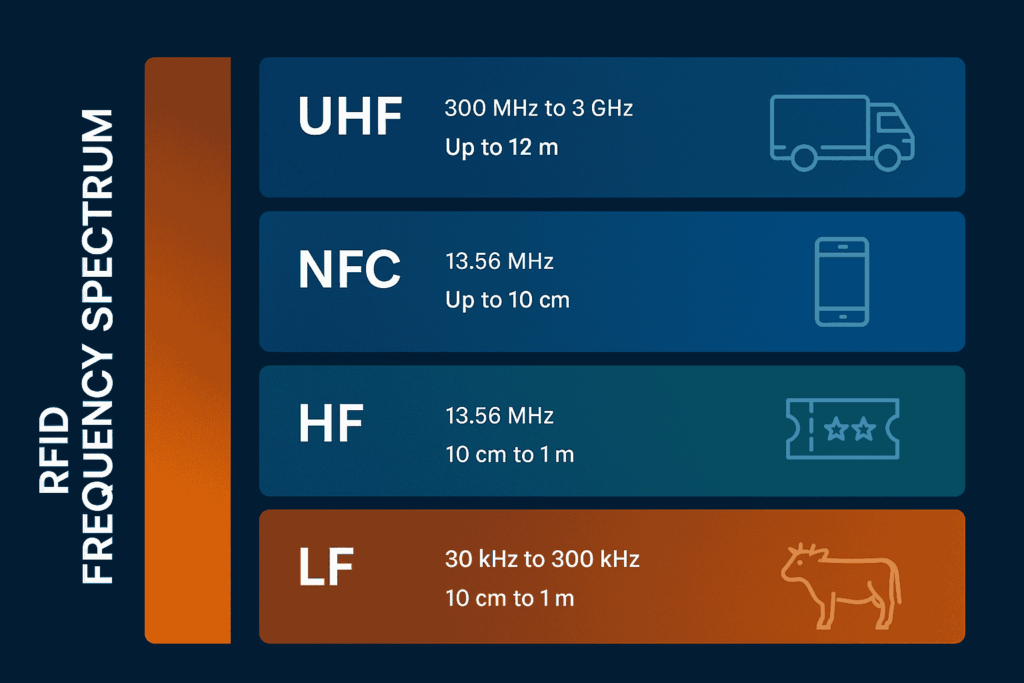
\includegraphics[width=0.8\textwidth]{image/section3/nfc.png} 
    \caption[NFC Frequency Spectrum Diagram]{NFC Frequency Spectrum Diagram (\textbf{Nguồn:} \href{https://altavantconsulting.com/fr/rfid-tag-comparison/}{Altavant})}
    \label{fig:nfc_frequency}
\end{figure}


Các đặc điểm kỹ thuật chính của NFC bao gồm:

\begin{table}[h]
\centering
\label{tab:nfc_specs}
\begin{tabular}{|l|l|}
\hline
\textbf{Thông số} & \textbf{Giá trị} \\
\hline
Tần số hoạt động & 13.56 MHz \\
Phạm vi truyền thông & < 10 cm (thông thường 4-5 cm) \\
Tốc độ truyền dữ liệu & 106, 212, 424, 848 kbps \\
Thời gian thiết lập kết nối & < 0.1 giây \\
Công suất tiêu thụ & Passive: 0 mW, Active: < 15 mA \\
Chuẩn hóa & ISO/IEC 14443, ISO/IEC 18092 \\
\hline
\end{tabular}
\caption{Thông số kỹ thuật của NFC \cite{coskun2013professional,iso14443,iso18092}}
\end{table}

Phạm vi hoạt động rất ngắn của NFC (nhỏ hơn 10 cm) là một đặc tính quan trọng giúp đảm bảo bảo mật ở mức vật lý (Physical security). Do yêu cầu thiết bị phải ở khoảng cách rất gần, kẻ tấn công gặp nhiều khó khăn trong việc nghe lén dữ liệu (Eavesdropping) hoặc thực hiện tấn công trung gian (MITM) trong quá trình giao tiếp \cite{haselsteiner2006security}.

\subsubsection{Nguyên lý hoạt động}

NFC hoạt động dựa trên nguyên lý \textbf{inductive coupling} (ghép nối cảm ứng) giữa hai cuộn dây antenna ở khoảng cách gần. Khi một thiết bị NFC (initiator/reader) phát ra từ trường RF tại tần số 13.56 MHz, từ trường này cảm ứng điện áp trong cuộn dây của thiết bị thụ động (target/tag), cung cấp năng lượng cho chip và cho phép truyền dữ liệu \cite{finkenzeller2010rfid}.

\begin{figure}[H]
    \centering
    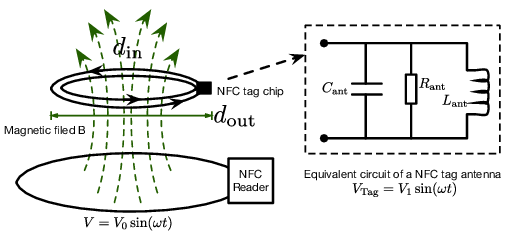
\includegraphics[width=0.8\textwidth]{image/section3/nfc2.png} 
    \caption[Sơ đồ minh họa trường từ tính giữa Reader và Tag]{Sơ đồ minh họa trường từ tính giữa Reader và Tag (\textbf{Nguồn:} \href{https://www.researchgate.net/publication/350040273_One_tag_two_codes_identifying_optical_barcodes_with_NFC}{ResearchGate})}
    \label{}
\end{figure}


Quá trình truyền dữ liệu được thực hiện thông qua cơ chế \textbf{điều chế tải} (\textit{load modulation}):

\begin{enumerate}
\item \textbf{Thiết bị đọc → Thẻ (Kênh truyền xuôi):}
Thiết bị đọc phát sóng mang tần số \textbf{13.56 MHz}, được điều chế bằng \textbf{ASK} (\textit{Amplitude Shift Keying – điều chế dịch biên độ}) với độ sâu điều chế \textbf{10\% hoặc 100\%} theo tiêu chuẩn \textbf{ISO/IEC 14443} loại A/B.

\item \textbf{Thẻ → Thiết bị đọc (kênh truyền ngược):}  
Thẻ thay đổi trở kháng của anten bằng cách bật hoặc tắt điện trở tải, tạo ra sự biến thiên điện áp trên cuộn dây của thiết bị đọc (cơ chế \textit{load modulation}). Thiết bị đọc phát hiện các thay đổi này và giải mã thành dữ liệu.
\end{enumerate}

Kỹ thuật này cho phép tag hoạt động ở chế độ passive (không cần pin) trong khi vẫn có thể truyền dữ liệu về reader \cite{coskun2013professional}.

\subsubsection{Ba chế độ hoạt động của NFC}

NFC hỗ trợ ba chế độ hoạt động chính theo chuẩn ISO/IEC 18092 \cite{iso18092}:
\par\vspace{0.5em}
\textbf{1. Reader/Writer Mode:}
\par\vspace{0.3em}
Trong chế độ này, thiết bị NFC hoạt động như một bộ đọc (Reader) để đọc và ghi dữ liệu từ các thẻ NFC thụ động (Passive NFC tags). Các ứng dụng phổ biến bao gồm:
\begin{itemize}
    \item Đọc \textbf{Smart poster} (thẻ NFC chứa địa chỉ web \textit{URL} hoặc nội dung văn bản)
    \item Đọc các thẻ theo chuẩn \textbf{NFC Forum Type~1--4}
    \item Ghi dữ liệu theo định dạng \textbf{NDEF (NFC Data Exchange Format)} lên thẻ
\end{itemize}

\begin{figure}[H]
    \centering
    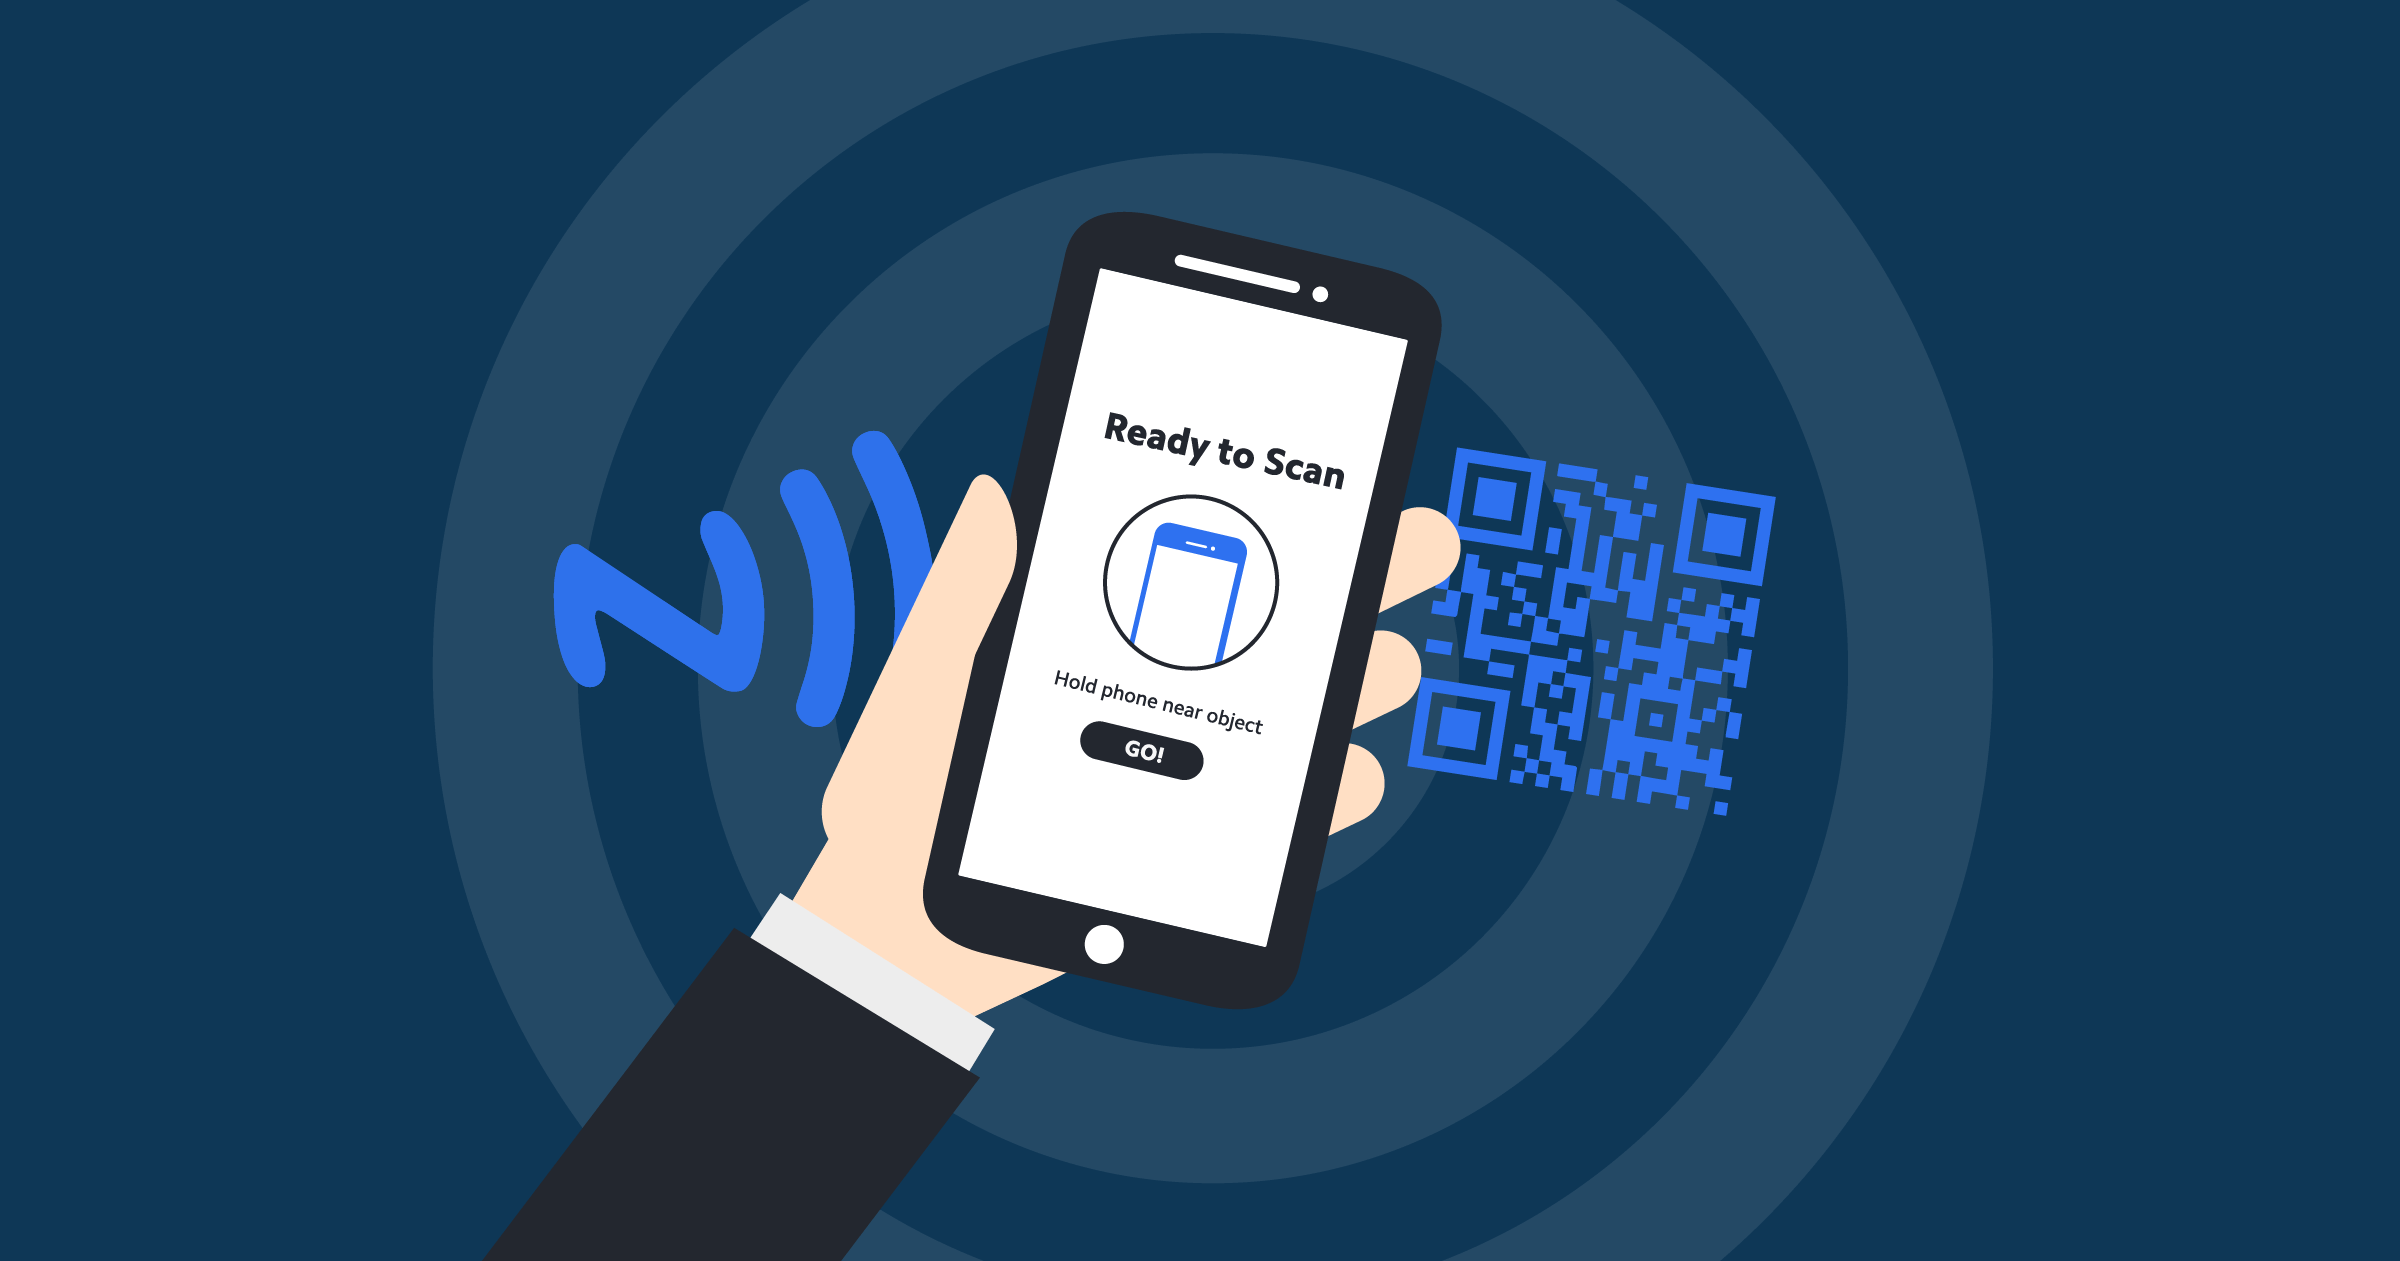
\includegraphics[width=0.8\textwidth]{image/section3/nfc3.png} 
    \caption[NFC Reader/Writer Mode]{NFC Reader/Writer Mode (\textbf{Nguồn:} \href{https://bluebite.medium.com/how-to-scan-nfc-tags-or-qr-codes-b71b8d92dd5}{Blue Bite})}
    \label{}
\end{figure}

\par\vspace{0.8em}
\textbf{2. Peer-to-Peer Mode (P2P):}

\par\vspace{0.3em}

Hai thiết bị NFC chủ động giao tiếp trực tiếp với nhau thông qua giao thức \textbf{LLCP (Logical Link Control Protocol)}. Trong quá trình trao đổi dữ liệu, hai thiết bị luân phiên phát trường sóng vô tuyến (RF field) theo cơ chế phân chia theo thời gian (Time-division multiplexing). Các ứng dụng tiêu biểu bao gồm:
\begin{itemize}
    \item \textbf{Android Beam}: truyền tệp và chia sẻ danh bạ
    \item Ghép nối \textbf{Bluetooth} thông qua cơ chế \textbf{NFC handover}
    \item Chia sẻ thông tin xác thực mạng \textbf{Wi-Fi}
\end{itemize}

\par\vspace{0.8em}
\textbf{3. Card Emulation Mode:}

\par\vspace{0.3em}
Thiết bị NFC (thường là điện thoại thông minh) giả lập một thẻ NFC hoặc thẻ thông minh (Smart card), cho phép tương tác trực tiếp với các thiết bị đầu cuối đã được triển khai sẵn trong hạ tầng. Hiện nay tồn tại hai hướng triển khai chính \cite{madlmayr2008nfc}:

\begin{itemize}
    \item \textbf{Dựa trên Secure Element (SE):} 
    Sử dụng phần cứng bảo mật chuyên dụng (embedded SE, thẻ SIM hoặc thẻ microSD) để lưu trữ dữ liệu nhạy cảm và thực hiện các phép toán mật mã. Cách tiếp cận này cung cấp mức độ bảo mật cao nhờ khả năng chống can thiệp vật lý, tuy nhiên quy trình cấp phát và quản lý khóa (Provisioning) phức tạp.

    \item \textbf{Host Card Emulation (HCE):} 
    Việc giả lập thẻ được thực hiện trực tiếp bởi bộ xử lý ứng dụng (Application processor – CPU chính của điện thoại thông minh) mà không cần sử dụng Secure Element. Nền tảng Android (từ phiên bản 4.4 trở lên) hỗ trợ HCE \cite{android_security}, và iOS (từ phiên bản 13 trở lên) cũng hỗ trợ HCE. Trong phạm vi đề tài này, HCE được lựa chọn để triển khai giai đoạn cấp phát khóa (Provisioning).
\end{itemize}

\begin{figure}[H]
    \centering
    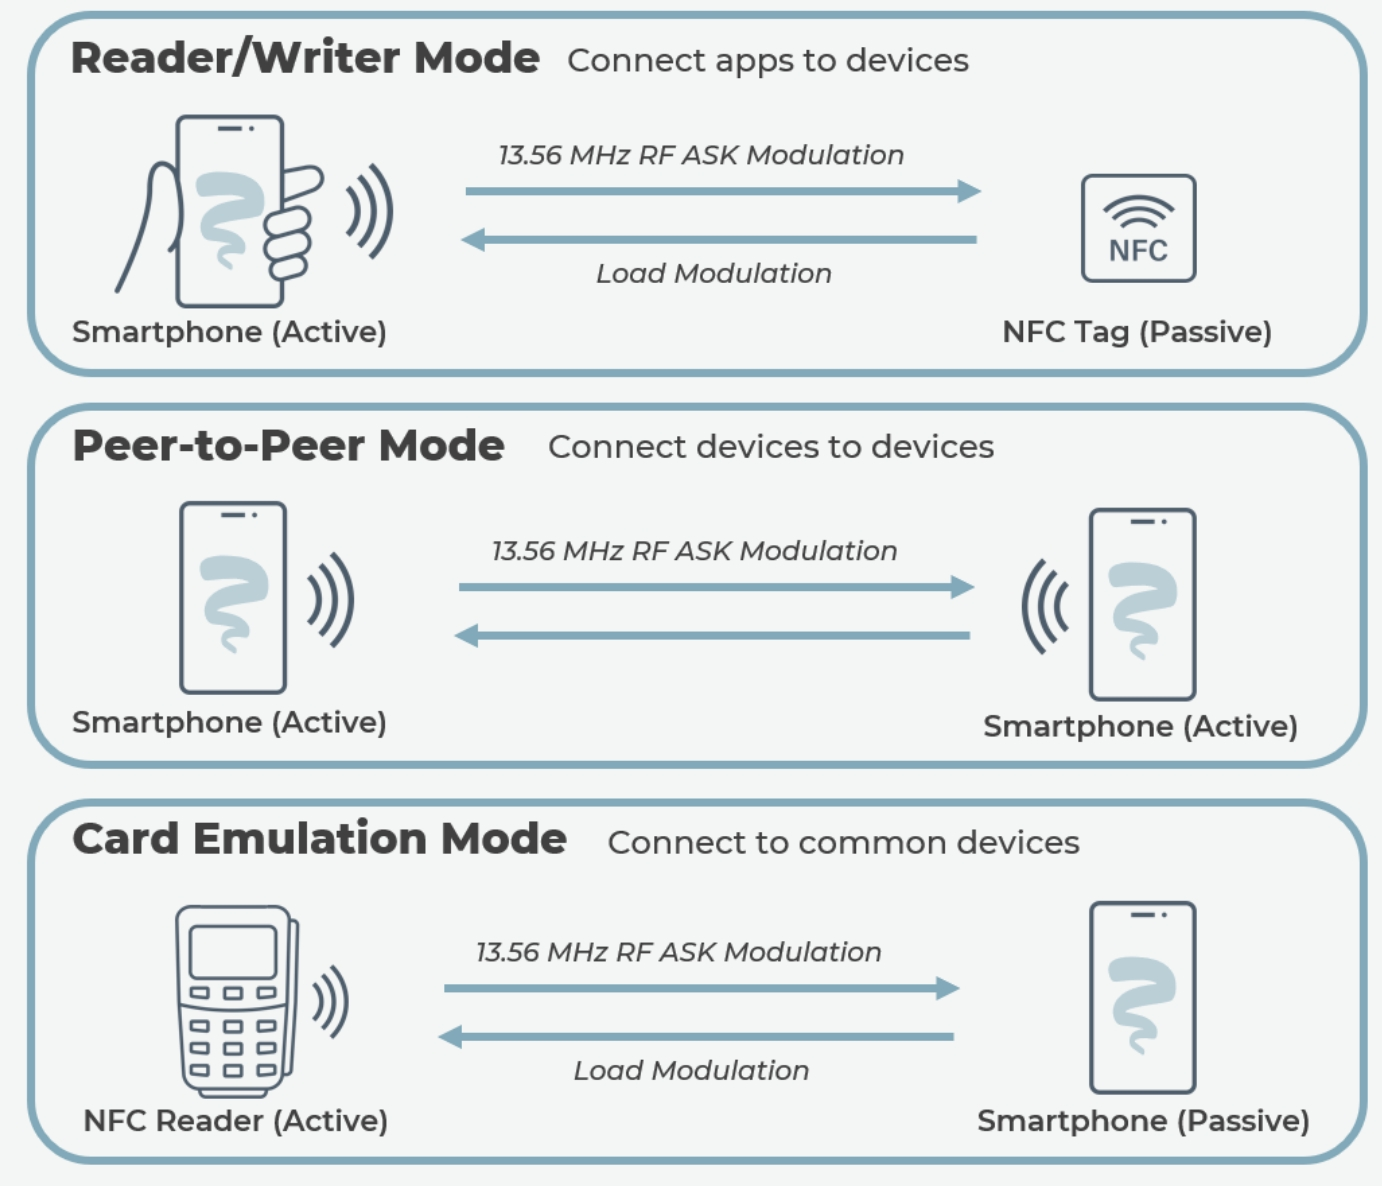
\includegraphics[width=0.8\textwidth]{image/section3/nfc4.jpeg} 
    \caption[So sánh 3 chế độ của NFC]{So sánh 3 chế độ của NFC (\textbf{Nguồn:} \href{https://www.cardinalpeak.com/blog/counterfeit-protection-exploring-the-role-of-nfc-in-the-iot}{Cardinal Peak})}
    \label{}
\end{figure}


\subsubsection{Giao thức APDU}

Trong chế độ giả lập thẻ (card emulation mode), giao tiếp giữa đầu đọc 
(reader) và thẻ (card) sử dụng \textbf{giao thức APDU (Application Protocol 
Data Unit)} theo chuẩn ISO/IEC 7816-4 \cite{iso7816}. APDU là đơn vị dữ 
liệu ở tầng ứng dụng cho phép truyền các lệnh và phản hồi  giữa hai thiết bị.

\textbf{Command APDU (từ reader → card):}

\begin{table}[h]
\centering
\label{tab:command_apdu}
\begin{tabular}{|l|l|l|}
\hline
\textbf{Field} & \textbf{Size} & \textbf{Mô tả} \\
\hline
CLA & 1 byte & Class byte (instruction class) \\
INS & 1 byte & Instruction byte (command) \\
P1 & 1 byte & Parameter 1 \\
P2 & 1 byte & Parameter 2 \\
Lc & 1 byte & Length of command data \\
Data & Variable & Command data (if Lc > 0) \\
Le & 1 byte & Expected response length \\
\hline
\end{tabular}
\caption{Cấu trúc Command APDU}
\end{table}

\textbf{Response APDU (từ card → reader):}

\begin{table}[h]
\centering
\label{tab:response_apdu}
\begin{tabular}{|l|l|l|}
\hline
\textbf{Field} & \textbf{Size} & \textbf{Mô tả} \\
\hline
Data & Variable & Response data \\
SW1 & 1 byte & Status word 1 \\
SW2 & 1 byte & Status word 2 \\
\hline
\end{tabular}
\caption{Cấu trúc Response APDU}
\end{table}

Status words (SW1 SW2) chỉ định kết quả xử lý command:
\begin{itemize}
    \item \texttt{90 00}: Success (Normal processing)
    \item \texttt{6A 82}: File not found
    \item \texttt{6A 86}: Incorrect parameters P1-P2
    \item \texttt{67 00}: Wrong length (Lc hoặc Le)
\end{itemize}

\textbf{Ví dụ: SELECT AID Command}

Để chọn một application trên NFC card, reader gửi SELECT command với Application Identifier (AID):

\noindent\begin{minipage}{\linewidth}
\begin{lstlisting}[language=C++, caption={NFC SELECT AID Command}]
Command:  00 A4 04 00 06 F0 01 02 03 04 05 00
          |  |  |  |  |  |              |  |
          |  |  |  |  |  |              |  Le (expected length)
          |  |  |  |  |  Data (AID: F00102030405)
          |  |  |  |  Lc (length = 6 bytes)
          |  |  P1 P2 (04 00 = select by name)
          |  INS (A4 = SELECT)
          CLA (00 = inter-industry class)

Response: 90 00
          |  |
          |  SW2
          SW1 (success)
\end{lstlisting}
\end{minipage}


\subsubsection{Bảo mật NFC}

NFC cung cấp một số đặc điểm bảo mật tự nhiên nhờ phạm vi hoạt động ngắn \cite{haselsteiner2006security}:
\par\vspace{0.5em}
\textbf{Ưu điểm:}
\begin{itemize}
    \item \textbf{Physical proximity:} Yêu cầu khoảng cách < 10 cm giảm thiểu bị nghe lén thông tin cá nhân
    \item \textbf{No pairing required:} Không cần setup phức tạp như Bluetooth
    \item \textbf{Fast connection:} Transaction time < 0.1s, khó can thiệp
\end{itemize}

\textbf{Các mối đe dọa và biện pháp:}
\begin{itemize}
    \item \textbf{Nghe lén (Eavesdropping):} 
    Kẻ tấn công có thể đặt ăng-ten ở khoảng cách gần để thu thập tín hiệu vô tuyến (RF signal) trong quá trình truyền dữ liệu. 

    
    \textit{Biện pháp:} Áp dụng cơ chế mã hóa ở tầng ứng dụng (Application layer), cụ thể trong đề tài này là sử dụng chữ ký số ECDSA để bảo vệ nội dung trao đổi.

    \item \textbf{Sửa đổi dữ liệu (Data Modification):} 
    Các tấn công chủ động (Active attack) có thể can thiệp và thay đổi dữ liệu trong quá trình truyền.

    
    \textit{Biện pháp:} Sử dụng chữ ký số (Digital signature) kết hợp với cơ chế kiểm tra toàn vẹn dữ liệu (Integrity checking).

    \item \textbf{Tấn công chuyển tiếp (Relay Attack):} 
    Kẻ tấn công sử dụng hai thiết bị trung gian để chuyển tiếp (Relay) quá trình giao tiếp giữa bộ đọc (Reader) và thẻ (Card) ở khoảng cách xa.

    
    \textit{Biện pháp:} Triển khai giao thức hỏi–đáp (challenge–response protocol) có gắn dấu thời gian (Timestamp); trong phạm vi đề tài, cơ chế này được hiện thực thông qua việc xác thực chữ ký ECDSA.
\end{itemize}


Theo nghiên cứu của Haselsteiner và Breitfuß (2006), công nghệ NFC có thể cung cấp mức độ bảo mật tương đương với thẻ thông minh tiếp xúc trực tiếp (Contact smart cards) khi được kết hợp với các giao thức mật mã phù hợp (Cryptographic protocols) \cite{haselsteiner2006security}.


\subsection{Bluetooth Low Energy - BLE}

\subsubsection{Giới thiệu và đặc điểm kỹ thuật}

Bluetooth Low Energy (BLE), còn được gọi là Bluetooth Smart, là phiên bản tiết kiệm năng lượng của Bluetooth Classic, được giới thiệu trong \textbf{Bluetooth 4.0 specification} năm 2010 bởi Bluetooth SIG (Special Interest Group) \cite{bluetooth40}. BLE được thiết kế đặc biệt cho các ứng dụng IoT yêu cầu battery life lâu (từ vài tháng đến vài năm) với cost thấp \cite{gomez2012overview,heydon2013bluetooth,townsend2014getting}.

\begin{figure}[H]
    \centering
    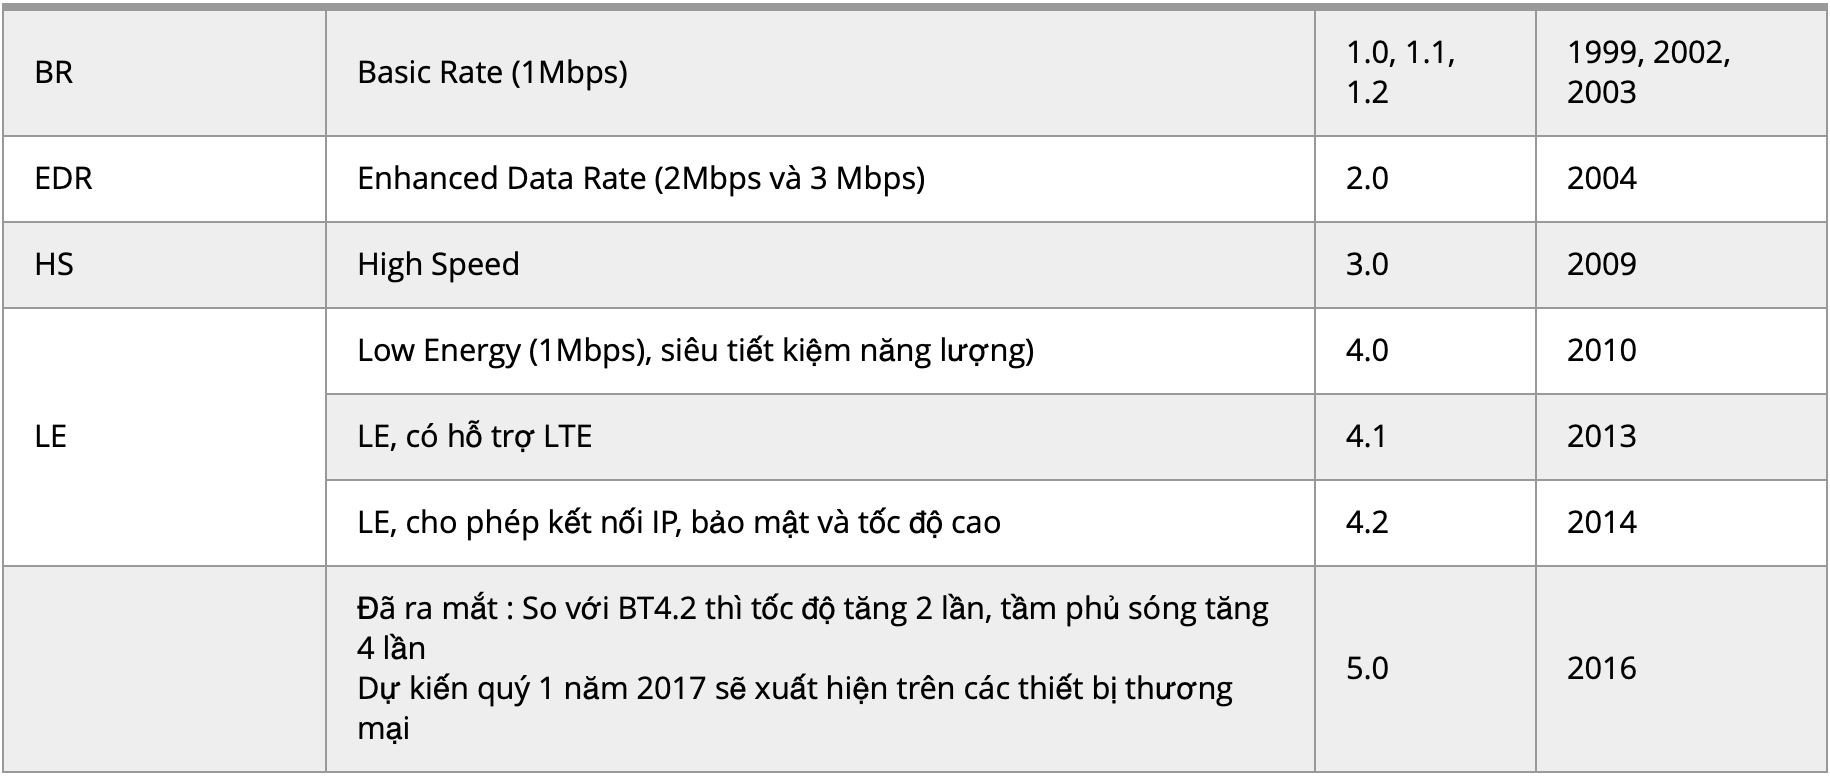
\includegraphics[width=0.8\textwidth]{image/section3/bluetooth2.png} 
    \caption[Sự phát triển của công nghệ Bluetooth qua các thời kỳ]{Sự phát triển của công nghệ Bluetooth qua các thời kỳ (\textbf{Nguồn:} \href{https://vngiotlab.github.io/vbluno/vi/mydoc_ble_vi.html}{VBLUno51 board})}
    \label{}
\end{figure}

\begin{table}[h]
\centering
\label{tab:ble_vs_classic}
\begin{tabular}{|l|l|l|}
\hline
\textbf{Đặc điểm} & \textbf{BLE} & \textbf{Bluetooth Classic} \\
\hline
Băng tần hoạt động & 2.4 GHz ISM & 2.4 GHz ISM \\
Số kênh truyền & 40 kênh (khoảng cách 2 MHz) & 79 kênh (khoảng cách 1 MHz) \\
Phạm vi hoạt động & 10--50 m (Class 2) & 10--100 m \\
Tốc độ dữ liệu & 1 Mbps (Bluetooth 4.x) & 1--3 Mbps \\
                & 2 Mbps (Bluetooth 5.x) &  \\
Độ trễ (Latency) & 6 ms & 100 ms \\
Dòng tiêu thụ cực đại & 15 mA & 30 mA \\
Công suất tiêu thụ & 0.01--0.5 W & 1 W \\
Ứng dụng điển hình & Cảm biến, thiết bị đeo & Âm thanh, truyền tệp \\
\hline
\end{tabular}
\caption{So sánh Bluetooth Low Energy (BLE) và Bluetooth Classic \cite{bluetooth40,ble_core,gomez2012overview}}
\end{table}


BLE sử dụng \textbf{40 kênh vô tuyến (RF channels)} trong băng tần \textbf{2.4 GHz} (từ 2.400 đến 2.4835 GHz) \cite{gomez2012overview}, bao gồm:

\begin{itemize}
    \item \textbf{3 kênh quảng bá (Advertising channels):} Các kênh 37, 38 và 39 (tương ứng với các tần số 2.402 GHz, 2.426 GHz và 2.480 GHz) được lựa chọn nhằm giảm thiểu nhiễu từ các kênh Wi-Fi phổ biến (kênh 1, 6 và 11).
    
    \item \textbf{37 kênh dữ liệu (Data channels):} Các kênh từ 0 đến 36 được sử dụng cho quá trình truyền dữ liệu sau khi các thiết bị đã thiết lập kết nối.
\end{itemize}


\begin{figure}[H]
    \centering
    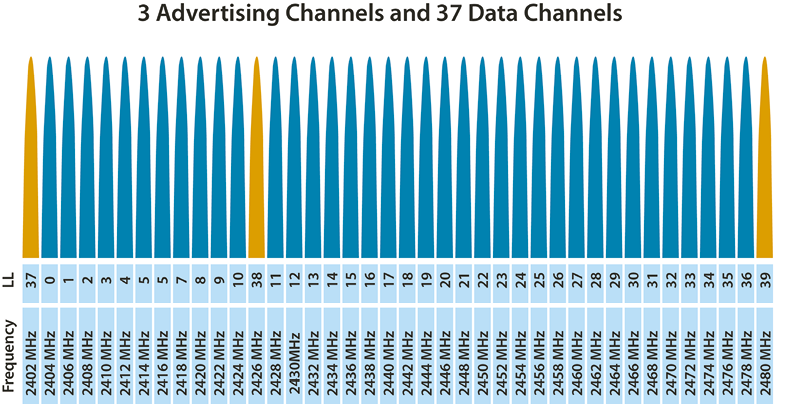
\includegraphics[width=0.8\textwidth]{image/section3/blemap.png} 
    \caption[Biểu đồ 40 kênh BLE]{Biểu đồ 40 kênh BLE (\textbf{Nguồn:} \href{https://www.researchgate.net/figure/Bluetooth-low-energy-channels-and-frequencies_fig7_310500994}{ResearchGate})}
    \label{fig:ble_channels}
\end{figure}


\subsubsection{Kiến trúc giao thức BLE}

Giao thức BLE được tổ chức thành nhiều tầng theo mô hình OSI 
\cite{townsend2014getting,bluetooth40}:

\begin{enumerate}
    \item \textbf{Tầng vật lý (Physical Layer - PHY):} 
    
    Xử lý bộ thu phát RF, điều chế tín hiệu GFSK (Gaussian Frequency Shift 
    Keying), và nhảy tần. Phiên bản BLE 5.0 bổ sung hai chế độ PHY mới: 
    2 Mbps cho tốc độ cao và 125/500 kbps cho khoảng cách xa 
    \cite{ble_core}.
    
    \item \textbf{Tầng liên kết (Link Layer - LL):}
    
    Quản lý quảng bá (Advertising), quét tìm (Scanning), thiết lập kết nối, 
    và truyền gói dữ liệu. Tầng này định nghĩa năm trạng thái thiết bị: 
    Standby, Advertising, Scanning, Initiating, và Connection 
    \cite{gomez2012overview}.
    
    \item \textbf{Giao diện điều khiển máy chủ (Host Controller Interface - HCI):}
    
    Cung cấp giao diện chuẩn hóa giữa máy chủ (application processor) và 
    bộ điều khiển (BLE chip), thường sử dụng UART, USB, hoặc SDIO 
    \cite{bluetooth40}.
    
    \item \textbf{Logical Link Control and Adaptation Protocol - L2CAP:}
    
    Thực hiện phân mảnh và tái lắp ráp gói tin, ghép kênh các giao thức, 
    và đảm bảo chất lượng dịch vụ. BLE sử dụng phiên bản L2CAP đơn giản 
    hóa so với Bluetooth Classic \cite{heydon2013bluetooth}.
    
    \item \textbf{Attribute Protocol - ATT:}
    
    Định nghĩa cách thức client truy cập các thuộc tính trên server thông 
    qua các thao tác Read, Write, Notify và Indicate. Mỗi thuộc tính có 
    handle (định danh 16-bit), type (UUID), và giá trị \cite{bluetooth40}.
    
    \item \textbf{Generic Attribute Profile - GATT:}
    
    Xây dựng trên ATT, định nghĩa cách tổ chức các thuộc tính thành dịch vụ 
    (Services) và đặc tính (Characteristics). GATT là tầng mà các nhà phát 
    triển thường tương tác trực tiếp \cite{townsend2014getting}.
    
    \item \textbf{Generic Access Profile - GAP:}
    
    Quản lý vai trò thiết bị (Central/Peripheral), quảng bá, khám phá 
    (Discovery), và các thủ tục kết nối \cite{heydon2013bluetooth}.
\end{enumerate}


\begin{figure}[H]
    \centering
    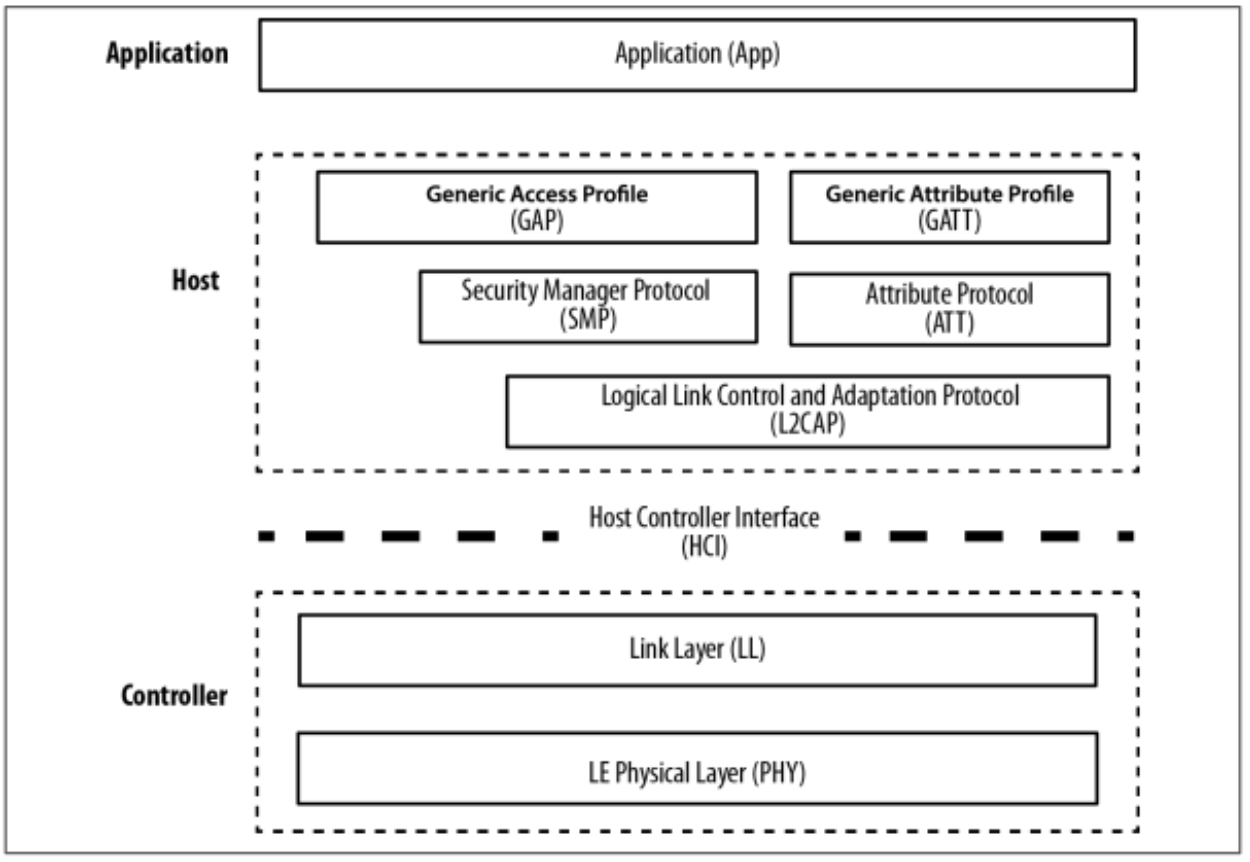
\includegraphics[width=0.8\textwidth]{image/section3/blue5.png} 
    \caption[Sơ đồ Layered Architecture của BLE]{Sơ đồ Layered Architecture của BLE (\textbf{Nguồn:} \href{https://www.researchgate.net/publication/379552583_Application_of_bluetooth_mesh_network_in_multi-device_system_management}{Researchgate})}
    \label{}
\end{figure}
\subsubsection{GATT (Generic Attribute Profile)}

GATT (Generic Attribute Profile) định nghĩa cấu trúc dữ liệu phân cấp
(Hierarchical data structure) cho các dịch vụ BLE \cite{heydon2013bluetooth}:

\noindent\begin{minipage}{\linewidth}
\begin{lstlisting}[language=C++, caption={Định nghĩa cấu trúc dữ liệu phân cấp}]
    Profile
     |
     +-- Service (UUID: 16-bit or 128-bit)
     |    |
     |    +-- Characteristic 1
     |    |    |
     |    |    +-- Value (data)
     |    |    +-- Properties (Read / Write / Notify / Indicate)
     |    |    +-- Descriptors (metadata)
     |    |         |
     |    |         +-- CCCD (Client Characteristic Configuration Descriptor)
     |    |
     |    +-- Characteristic 2
     |
     +-- Characteristic 3
\end{lstlisting}
\end{minipage}



\textbf{UUID (Universally Unique Identifier – Định danh duy nhất toàn cục):}
\begin{itemize}
    \item \textbf{UUID 16-bit:}  
    Được Bluetooth SIG quy định sẵn (Reserved) cho các dịch vụ chuẩn
    (ví dụ: Heart Rate Service = 0x180D).  
    Base UUID tương ứng:
    \texttt{0000xxxx-0000-1000-8000-00805F9B34FB}
    
    \item \textbf{UUID 128-bit:}  
    Được định nghĩa tùy chỉnh cho các dịch vụ hoặc Characteristic riêng
    do nhà phát triển thiết kế.  
    Ví dụ:
    \texttt{0000aaaa-1234-5678-9abc-def012345678}
\end{itemize}


\textbf{Thuộc tính của Characteristic (Characteristic Properties):}
\begin{table}[htbp]
\centering
\label{tab:gatt_properties}
\begin{tabular}{|l|p{10cm}|}
\hline
\textbf{Thuộc tính} & \textbf{Mô tả} \\
\hline
Read & Thiết bị Client đọc giá trị (value) thông qua bản tin ATT Read Request \\
Write & Thiết bị Client ghi giá trị và nhận phản hồi xác nhận từ server (ATT Write Request) \\
Write Without Response & Thiết bị Client ghi giá trị mà không cần chờ phản hồi xác nhận (ATT Write Command) \\
Notify & Thiết bị Server chủ động gửi dữ liệu đến client mà không yêu cầu xác nhận \\
Indicate & Thiết bị Server gửi dữ liệu đến client và yêu cầu xác nhận đã nhận (ATT Handle Value Confirmation) \\
\hline
\end{tabular}
\caption{Các thuộc tính của GATT Characteristic}
\end{table}


\textbf{Ví dụ: Heart Rate Service}

\noindent\begin{minipage}{\linewidth}
\begin{lstlisting}[language=C++, caption={Heart Rate Service}]
      Service: Heart Rate (0x180D)
       |
       +-- Characteristic: Heart Rate Measurement (0x2A37)
       |    |
       |    +-- Value: [0x16, 0x4E] -> 78 bpm
       |    +-- Properties: Notify
       |    +-- Descriptor: CCCD (0x2902)
       |         |
       |         +-- Value: [0x01, 0x00] -> Notifications enabled
       |
       +-- Characteristic: Body Sensor Location (0x2A38)
             |
             +-- Value: [0x01] -> Wrist
             +-- Properties: Read
\end{lstlisting}
\end{minipage}


\begin{figure}[H]
    \centering
    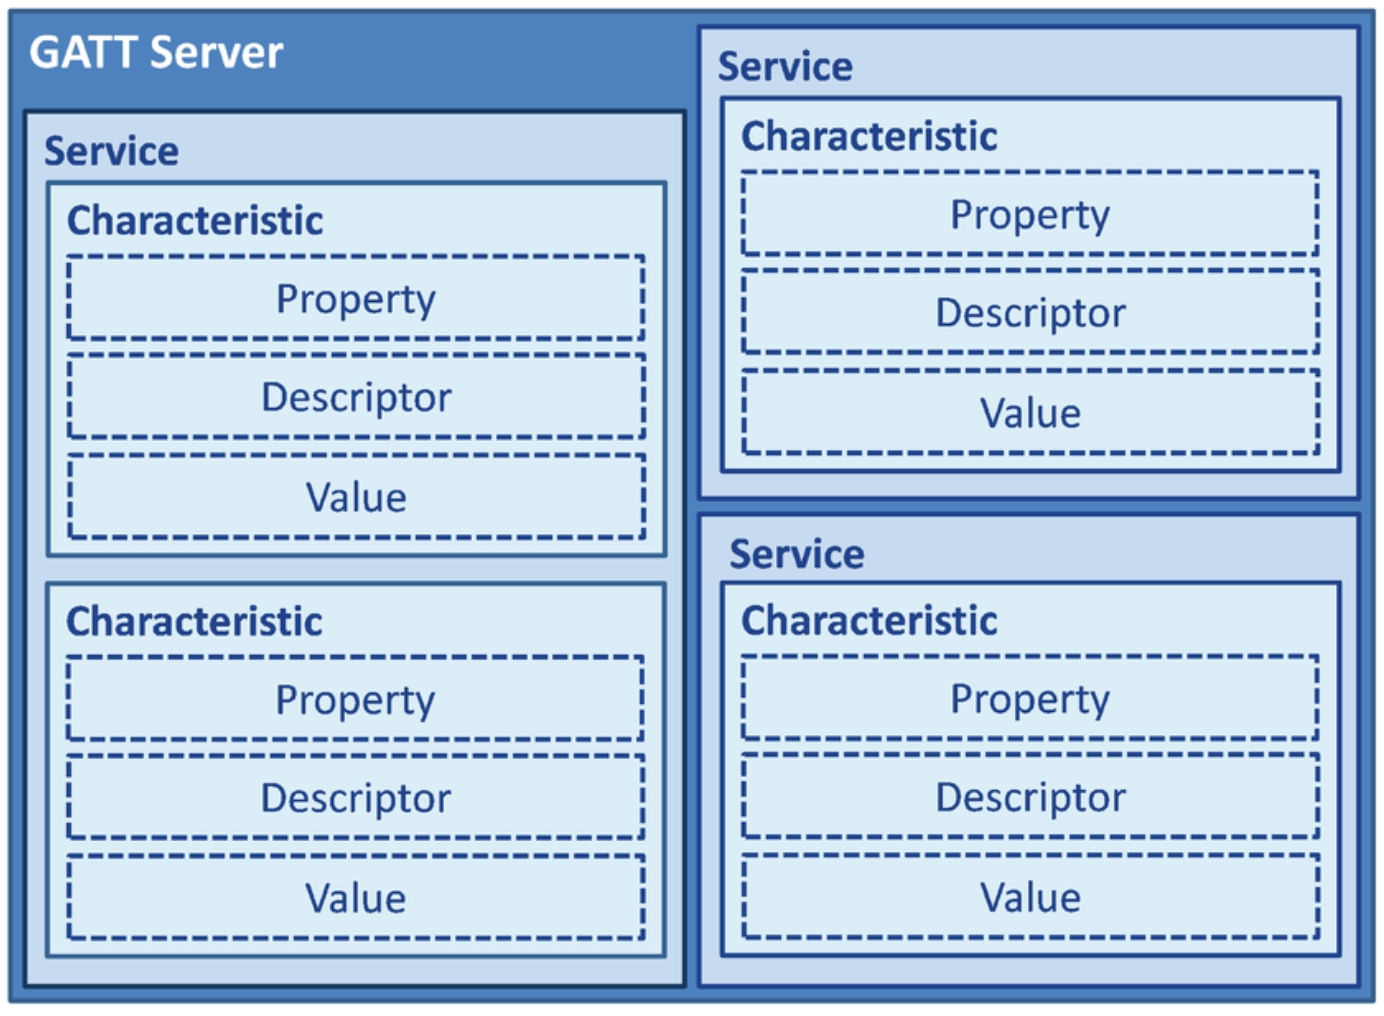
\includegraphics[width=0.8\textwidth]{image/section3/gatt.jpeg} 
    \caption[Diagram GATT Hierarchy]{Diagram GATT Hierarchy (\textbf{Nguồn:} \href{https://www.mdpi.com/1424-8220/17/12/2898}{MDPI})}
    \label{}
\end{figure}

\begin{itemize}
    \item \textbf{Handshake Write:} Smartphone gửi \emph{Ephemeral public key} kèm theo \emph{chữ ký số (Signature)} để khởi tạo phiên xác thực.
    
    \item \textbf{Handshake Read:} Smartphone đọc \emph{Ephemeral public key} do ECU sinh ra để hoàn tất quá trình trao đổi khóa tạm thời.

    \item \textbf{Status:} ECU sử dụng cơ chế \emph{Notify} để thông báo trạng  thái xác thực, bao gồm \texttt{AUTH\_SUCCESS} hoặc \texttt{AUTH\_FAILED}.

    \item \textbf{Challenge Read:} Smartphone nhận \emph{Challenge} do ECU tạo ra nhằm chống các hình thức tấn công giả mạo hoặc Relay attack.

    \item \textbf{Challenge Write:} Smartphone gửi lại \emph{chữ ký số của Challenge} để ECU kiểm tra và xác thực danh tính.
\end{itemize}

\subsubsection{Connection và Data Transfer Flow}

Quá trình thiết lập kết nối và truyền dữ liệu trong BLE bao gồm các bước chính sau đây \cite{townsend2014getting}:

\medskip
\par\vspace{0.5em}
\textbf{1. Advertising:}
\par\vspace{0.3em}
Ở giai đoạn này, thiết bị ngoại vi (Peripheral – trong đề tài là ESP32) định kỳ phát các Advertising packet trên 3 kênh quảng bá (Advertising channels).
Chu kỳ phát (Advertising interval) có thể cấu hình trong khoảng từ 20 ms đến 10.24 s \cite{bluetooth40,ble_core}.

Nội dung của Advertising packet bao gồm:
\begin{itemize}
\item Địa chỉ thiết bị (Sevice address), có thể là public address hoặc Random address
\item Tên thiết bị (Device name)
\item Danh sách các Service UUID mà thiết bị hỗ trợ
\item Mức công suất phát (TX power level)
\item Các cờ trạng thái (Flags), chẳng hạn như khả năng khám phá hoặc kết nối
\end{itemize}

\medskip
\par\vspace{0.5em}
\textbf{2. Scanning:}
\par\vspace{0.3em}
Thiết bị trung tâm (Central – smartphone) thực hiện lắng nghe các Advertising packet trên 3 Advertising channels để phát hiện thiết bị BLE ở gần.

BLE hỗ trợ hai chế độ quét (Scan mode):
\begin{itemize}
\item \textbf{Passive scanning:} Thiết bị trung tâm chỉ lắng nghe các Advertising packet mà không gửi phản hồi.

\item \textbf{Active scanning:} Sau khi nhận Advertising packet, thiết bị trung tâm gửi gói \texttt{SCAN\_REQ} để yêu cầu thêm thông tin, và Peripheral sẽ phản hồi bằng gói \texttt{SCAN\_RSP}.


\end{itemize}

\begin{figure}[H]
    \centering
    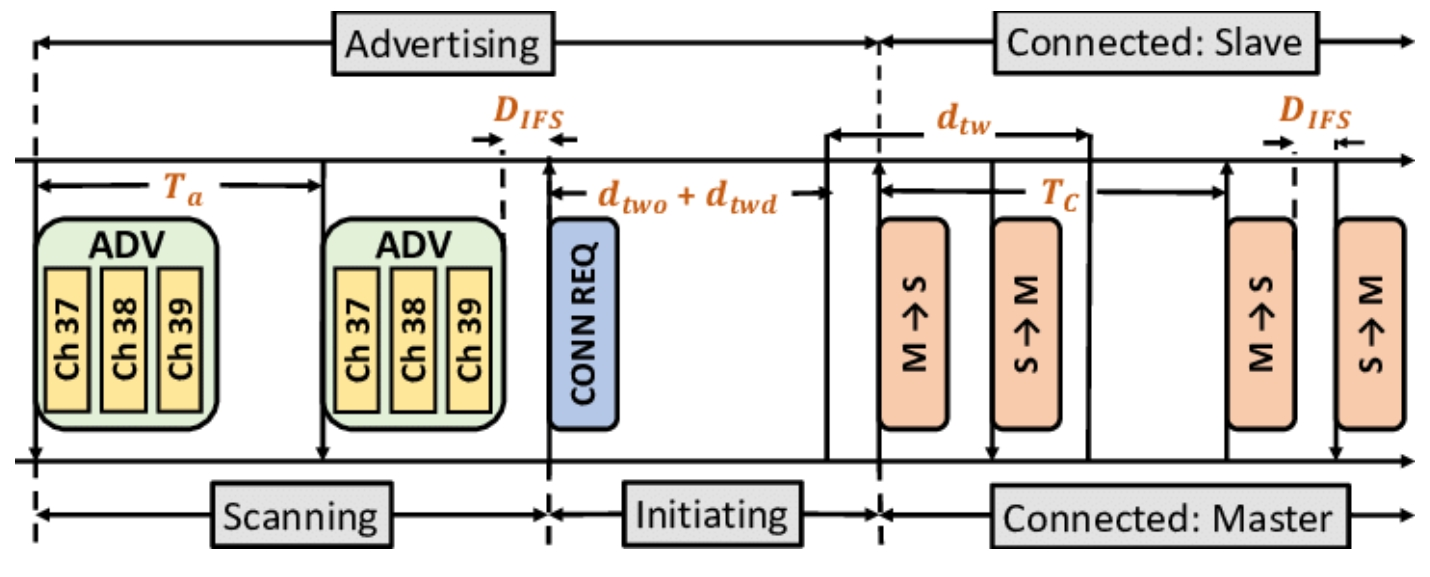
\includegraphics[width=0.8\textwidth]{image/section3/ble_flow.jpeg} 
    \caption[BLE Connection Flow]{BLE Connection Flow (\textbf{Nguồn:} \href{https://www.researchgate.net/publication/334783317_A_Robust_Algorithm_for_Sniffing_BLE_Long-Lived_Connections_in_Real-time}{ResearchGate})}
    \label{}
\end{figure}

\subsubsection{Bảo mật BLE}

BLE cung cấp nhiều cơ chế bảo mật ở tầng liên kết (Link layer) nhằm đảm bảo tính bí mật và toàn vẹn của dữ liệu \cite{bluetooth40}.

\medskip
\par\vspace{0.5em}
\textbf{1. Các phương thức ghép cặp (Pairing Methods):}
\par\vspace{0.3em}
BLE hỗ trợ nhiều phương thức ghép cặp với mức độ bảo mật khác nhau:
\begin{itemize}
\item \textbf{Just Works:}
Không cung cấp cơ chế bảo vệ chống tấn công trung gian (MITM – Man-In-The-Middle), chỉ hỗ trợ mã hóa dữ liệu sau khi ghép cặp. Phương thức này dễ bị nghe lén thụ động (Passive eavesdropping).

\item \textbf{Passkey Entry:}  
Người dùng nhập mã PIN gồm 6 chữ số để xác thực. Phương thức này có khả năng chống MITM, tuy nhiên mức độ an toàn phụ thuộc vào Entropy của mã PIN.

\item \textbf{Numeric Comparison:}  
Người dùng xác nhận hai thiết bị hiển thị cùng một mã số gồm 6 chữ số. Phương thức này cung cấp khả năng chống MITM hiệu quả và được xem là an toàn hơn so với Passkey Entry.

\item \textbf{Out-of-Band (OOB):}  
Sử dụng một kênh giao tiếp khác (ví dụ: NFC hoặc mã QR) để trao đổi dữ liệu xác thực. Đây là phương thức có mức độ bảo mật cao nhất và khả năng chống MITM tốt.

\end{itemize}

\medskip
\par\vspace{0.5em}
\textbf{2. Các mức bảo mật (Security Levels):}
\par\vspace{0.3em}
Chuẩn BLE định nghĩa bốn mức bảo mật như sau:
\begin{itemize}
\item \textbf{Level 1:} Không có bảo mật (không mã hóa, không xác thực)
\item \textbf{Level 2:} Ghép cặp không xác thực nhưng có mã hóa
\item \textbf{Level 3:} Ghép cặp có xác thực và có mã hóa
\item \textbf{Level 4:} Ghép cặp xác thực sử dụng LE Secure Connections (ECDH, Bluetooth 4.2 trở lên)
\end{itemize}

\medskip
\par\vspace{0.5em}
\textbf{3. LE Secure Connections (Bluetooth 4.2+):}
\par\vspace{0.3em}
Cơ chế LE Secure Connections sử dụng thuật toán trao đổi khóa ECDH với đường cong Elliptic P-256 thay cho giao thức ghép cặp cũ (Legacy pairing).
Phương pháp này cung cấp:
\begin{itemize}
\item Tính bảo mật chuyển tiếp (Forward secrecy)
\item Khả năng chống tấn công MITM thông qua cơ chế Numeric Comparison
\end{itemize}

\medskip
\textbf{Hạn chế:}

Mặc dù BLE cung cấp nhiều cơ chế bảo mật, trên thực tế nhiều hệ thống triển khai không đầy đủ hoặc sử dụng phương thức \textbf{Just Works} do tính đơn giản, dẫn đến thiếu khả năng chống MITM.
Nghiên cứu của Ryan (2013) đã chỉ ra nhiều lỗ hổng xuất phát từ việc triển khai không an toàn các cơ chế bảo mật BLE \cite{ryan2013bluetooth}.

\medskip
\textbf{Trong đề tài này:}

Cơ chế bảo mật được triển khai ở tầng ứng dụng (Application layer), hoạt động độc lập với cơ chế ghép cặp mặc định của BLE.
Hệ thống sử dụng kết hợp ECDH và HMAC để thực hiện xác thực hai chiều (Mutual authentication), không phụ thuộc vào các cơ chế bảo mật tích hợp sẵn của BLE.






%-----------------------------------------------------------------------





\subsection{Ultra-Wideband - UWB}
\subsubsection{Giới thiệu và đặc điểm kỹ thuật}
Ultra-Wideband (UWB) là công nghệ truyền thông không dây sử dụng \textbf{băng thông cực rộng} (lớn hơn 500 MHz) với \textbf{công suất phát rất thấp}, được trải trên một dải phổ tần rộng từ \textbf{3.1 đến 10.6 GHz} \cite{ieee802154}.
Khác với các công nghệ truyền thông băng hẹp truyền thống, UWB không tập trung năng lượng vào một tần số cụ thể mà phân bố mật độ công suất thấp trên toàn bộ dải tần, giúp giảm nhiễu và tăng khả năng đồng tồn tại với các hệ thống vô tuyến khác.

UWB được chuẩn hóa bởi các chuẩn \textbf{IEEE 802.15.4a} và \textbf{IEEE 802.15.4z}, trong đó bổ sung các cơ chế nâng cao cho định vị chính xác và bảo mật. Công nghệ này đã được \textbf{FCC (Federal Communications Commission)} phê duyệt cho sử dụng không cần cấp phép (Unlicensed use) từ năm 2002 \cite{fcc2002}.

\begin{figure}[H]
    \centering
    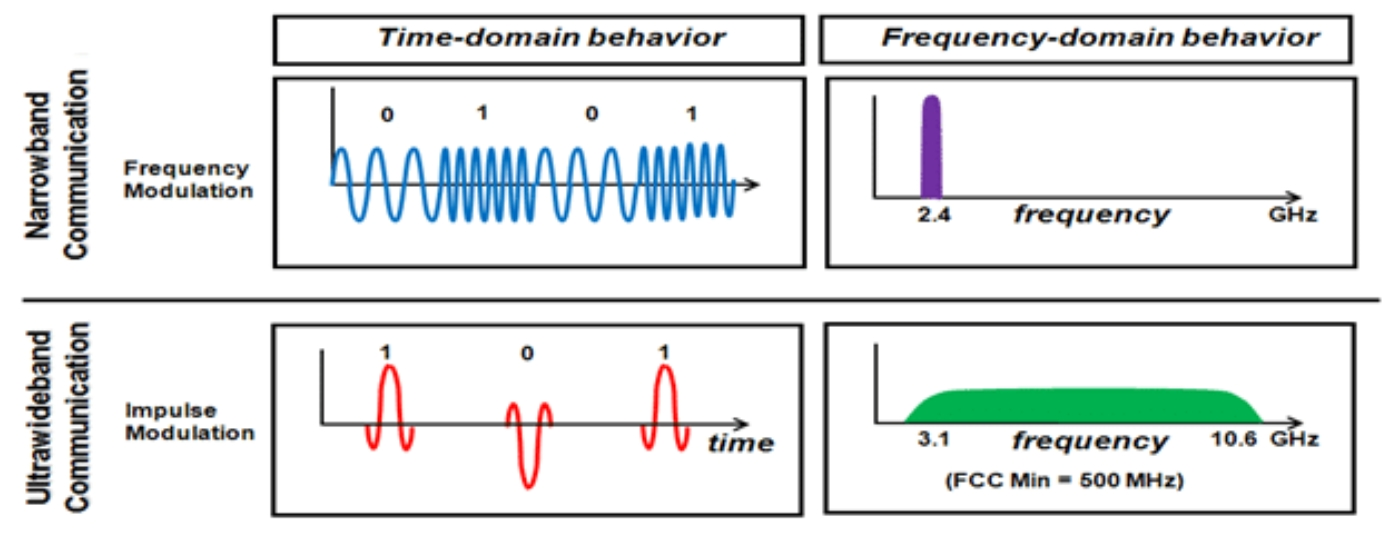
\includegraphics[width=0.8\textwidth]{image/section3/uwb.jpeg} 
    \caption[UWB Spectrum vs Narrowband]{UWB Spectrum vs Narrowband (\textbf{Nguồn:} \href{https://sirinsoftware.com/blog/uwb-technology-review-modules-characteristics-usage-perspectives}{Sirin Software})}
    \label{}
\end{figure}

\begin{table}[h]
\centering
\label{tab:uwb_specs}
\begin{tabular}{|l|l|}
\hline
\textbf{Thông số} & \textbf{Giá trị} \\ 
\hline
Băng tần hoạt động & 3.1--10.6 GHz (nhiều băng tần con) \\ 
Băng thông & > 500 MHz (thường 500--1000 MHz) \\ 
Phạm vi hoạt động & 10--200 m (trong nhà / ngoài trời) \\ 
Tốc độ dữ liệu & 110 kbps -- 27 Mbps \\ 
Độ chính xác định vị & 10--30 cm (thông thường), < 10 cm (tối ưu) \\ 
Công suất tiêu thụ & < 100 mW (điển hình) \\ 
Độ trễ & < 1 ms (cho đo khoảng cách) \\ 
Chuẩn hóa & IEEE 802.15.4a/z, FiRa Consortium \\ 
\hline
\end{tabular}
\caption{Thông số kỹ thuật của UWB}
\end{table}


\subsubsection{Nguyên lý hoạt động}

UWB truyền dữ liệu bằng cách phát các \textbf{xung vô tuyến cực ngắn} (\textit{Impulse radio pulses}) có độ rộng rất nhỏ (nhỏ hơn 1 ns) và chu kỳ hoạt động thấp, thay vì phát sóng liên tục (\textit{Continuous wave}) như Wi-Fi hoặc Bluetooth \cite{ghavami2007ultra}.


\begin{tabular}{ll}
a & Đạo hàm bậc năm của hàm Gaussian \\
b & Xung Gaussian đơn chu kỳ (Gaussian monocycle) \\
c & Xung Gaussian đơn chu kỳ sau khi qua bộ lọc \\
d & Phổ tương ứng được chuẩn hóa theo mặt nạ phổ FCC
\end{tabular}

\begin{figure}[H]
    \centering
    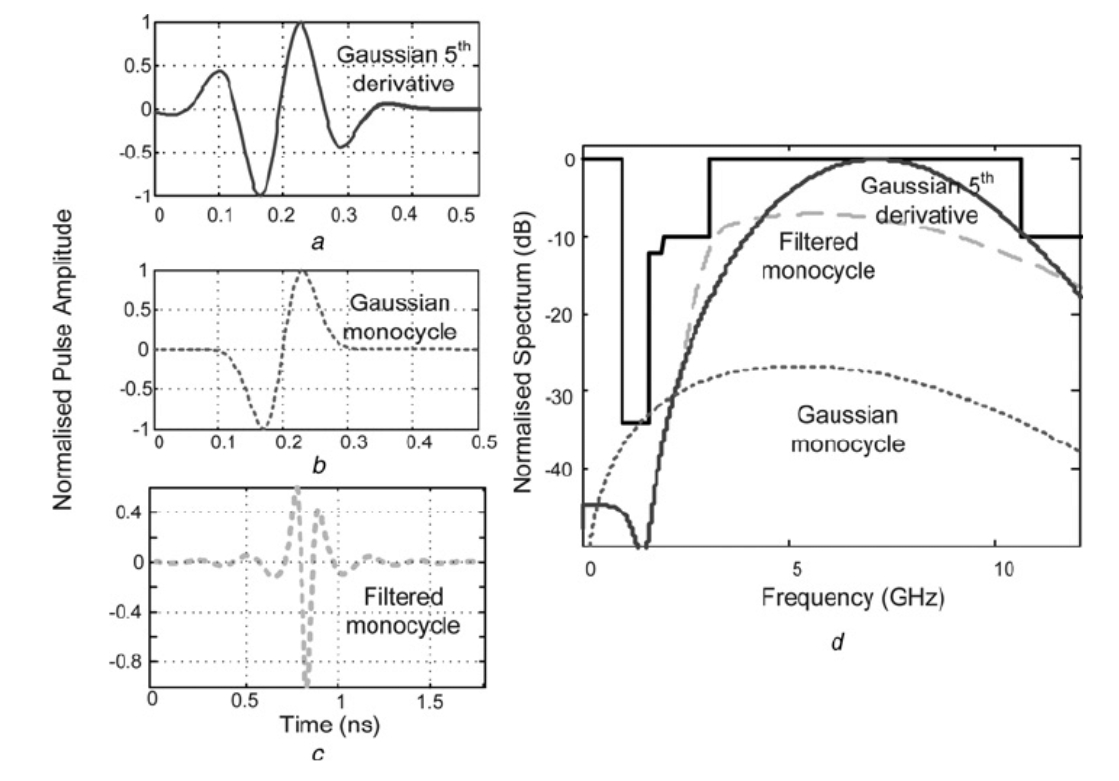
\includegraphics[width=0.8\textwidth]{image/section3/uwb2.jpeg} 
    \caption[Dạng sóng miền thời gian của xung UWB (Gaussian monocycle)]{Dạng sóng miền thời gian của xung UWB (Gaussian monocycle) (\textbf{Nguồn:} \href{https://www.researchgate.net/publication/260673659_Ultra-wideband_pulse_shaping_bypassing_the_inherent_limitations_of_the_Gaussian_monocycle}{ResearchGate})}
    \label{}
\end{figure}

\par\vspace{1em}
\textbf{Các đặc điểm quan trọng của công nghệ UWB bao gồm:}
\par\vspace{0.5em}
\textbf{1. Đo thời gian truyền sóng (TOF):}
\par\vspace{0.3em}
UWB có khả năng đo khoảng cách với độ chính xác cao dựa trên thời gian sóng điện từ truyền từ thiết bị phát đến thiết bị thu và quay trở lại. Khoảng cách được tính theo công thức:

\begin{equation}
d = \frac{c \cdot \Delta t}{2}
\end{equation}

Trong đó:
\begin{itemize}
    \item $d$: Khoảng cách giữa hai thiết bị (m)
    \item $c$: Tốc độ ánh sáng trong chân không ($3 \times 10^8$ m/s)
    \item $\Delta t$: Thời gian truyền hai chiều (\textit{Round-trip time}) (s)
\end{itemize}

Với độ chính xác đo thời gian ở mức khoảng 1 ns, UWB có thể đạt độ chính xác đo khoảng cách vào khoảng 30 cm. Các kỹ thuật nâng cao như đo dựa trên pha (\textit{Phase-based ranging}) hoặc chế độ chuỗi huấn luyện bảo mật (\textit{Scrambled Timestamp Sequence -- STS}) có thể cải thiện độ chính xác xuống dưới 10 cm \cite{decawave2017}.
\par\vspace{0.5em}
\textbf{2. Đo khoảng cách hai chiều đối xứng (DS-TWR):}
\par\vspace{0.3em}
Theo lý thuyết cơ bản, khoảng cách có thể được tính bằng phương pháp đo một vòng (Single-Sided TWR - SS-TWR) thông qua việc trao đổi hai gói tin. Tuy nhiên, SS-TWR gặp phải sai số rất lớn do sự trôi dạt xung nhịp (Clock drift) giữa bộ dao động thạch anh của hai thiết bị độc lập (điện thoại và ECU). Để khắc phục triệt để sai số này và tuân thủ chuẩn bảo mật CCC Digital Key Release 3.0, hệ thống bắt buộc sử dụng giao thức \textbf{Symmetrical Double-Sided Two-Way Ranging (DS-TWR)}.

Giao thức DS-TWR yêu cầu trao đổi 3 gói tin (\textit{Poll, Response, Final}) để tự động bù trừ sai lệch thời gian phần cứng. Trình tự thực hiện như sau:

\begin{enumerate}
    \item \textbf{Khởi tạo (Poll):} Thiết bị A (Initiator/Smartphone) phát gói \textit{Poll} và ghi nhận thời gian phát. Thiết bị B (Responder/ECU) nhận gói tin và ghi lại thời gian đến.
    \item \textbf{Phản hồi (Response):} Sau một khoảng thời gian trễ xử lý ($T_{reply1}$), Thiết bị B phát gói \textit{Response}. Thiết bị A nhận gói tin này và tính toán được thời gian truyền vòng đầu tiên ($T_{round1}$).
    \item \textbf{Chốt chặng (Final):} Sau khoảng thời gian trễ xử lý ($T_{reply2}$), Thiết bị A phát gói \textit{Final} mang theo dữ liệu về các mốc thời gian của nó. Thiết bị B nhận gói \textit{Final} và tính toán được thời gian truyền vòng thứ hai ($T_{round2}$).
\end{enumerate}

\begin{figure}[H]
    \centering
    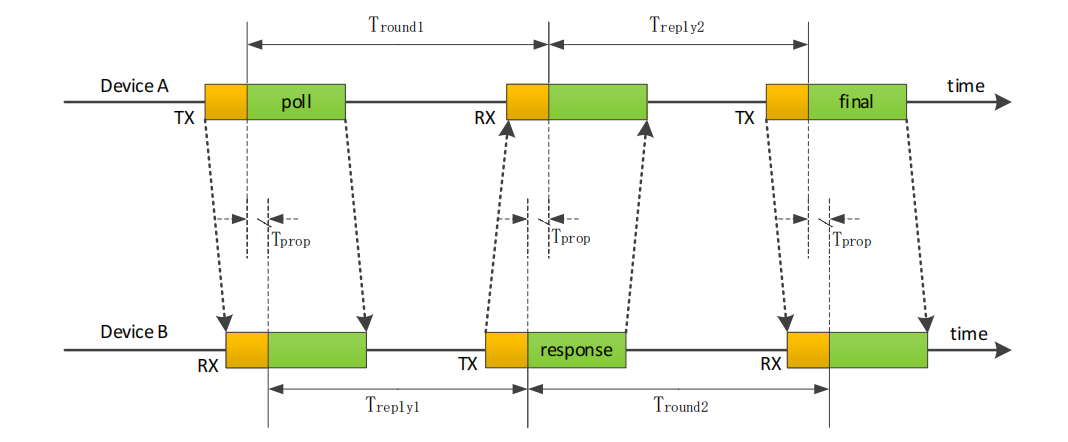
\includegraphics[width=0.7\textwidth]{image/section3/dstwr_protocol.png} 
    \caption[Sơ đồ trao đổi gói tin của giao thức Symmetrical DS-TWR]{Sơ đồ trao đổi gói tin của giao thức Symmetrical DS-TWR (\textbf{Nguồn:} \href{https://www.lansitec.com/uwb-positioning-technology/}{Lansitec})}
    \label{fig:dstwr_protocol}
\end{figure}

Thời gian truyền sóng thực sự (Time-of-Flight - ToF) được tính toán bằng công thức:
\begin{equation}
\text{ToF} = \frac{T_{round1} \times T_{round2} - T_{reply1} \times T_{reply2}}{T_{round1} + T_{round2} + T_{reply1} + T_{reply2}}
\end{equation}

Trong đó:
\begin{itemize}
    \item $T_{round1}$: Thời gian đo tại A, từ khi gửi \textit{Poll} đến khi nhận \textit{Response}.
    \item $T_{reply1}$: Thời gian xử lý tại B, từ khi nhận \textit{Poll} đến khi gửi \textit{Response}.
    \item $T_{round2}$: Thời gian đo tại B, từ khi gửi \textit{Response} đến khi nhận \textit{Final}.
    \item $T_{reply2}$: Thời gian xử lý tại A, từ khi nhận \textit{Response} đến khi gửi \textit{Final}.
\end{itemize}

Nhờ việc lấy tích chéo và chia cho tổng thời gian của cả hai vòng truyền, phương pháp DS-TWR triệt tiêu được hoàn toàn sai số bậc nhất (first-order error) sinh ra bởi sự chênh lệch tần số đồng hồ ($\Delta f$) giữa Smartphone và vi mạch UWB DW3000 trên xe. Điều này giúp hệ thống đạt được độ chính xác định vị ở mức centimet ($< 10$ cm) mà không cần chia sẻ chung một nguồn xung nhịp vật lý \cite{neirynck2016overview}.
\par\vspace{0.5em}

\textbf{3. Xác định góc đến của tín hiệu (AoA):}
\par\vspace{0.3em}
UWB có thể xác định góc đến của tín hiệu thông qua hệ thống nhiều anten (\textit{Antenna array}), cho phép thực hiện chức năng \textbf{xác định hướng} (\textit{Direction finding}) \cite{bharadwaj2020accurate}. Khi kết hợp với đo khoảng cách, hệ thống có thể thực hiện \textbf{định vị chính xác} (\textit{Precise positioning}) trong không gian ba chiều.

\subsubsection{Đo khoảng cách đa điểm (One-to-Many Ranging)}

Để định vị được thiết bị trong mặt phẳng quanh xe (như mục Định vị đa mỏ neo và Trilateration trình bày), hệ thống cần thu thập \textbf{đồng thời} nhiều khoảng cách $d_0, d_1, d_2$ từ một điện thoại đến nhiều mỏ neo trong \textbf{cùng một vòng đo} (ranging round). Việc lặp tuần tự nhiều phiên đo một–một (one-to-one DS-TWR) không đáp ứng được yêu cầu này vì hai lý do: (i) mỗi phiên DS-TWR riêng lẻ tiêu tốn một khoảng thời gian cố định nên tổng thời gian để đo lần lượt $N$ mỏ neo tăng tuyến tính theo $N$, làm giảm tần suất cập nhật vị trí; và (ii) các khoảng cách thu được tại các thời điểm khác nhau sẽ không đồng bộ về mặt thời gian, dẫn đến sai số đáng kể khi thiết bị đang chuyển động và làm suy giảm tính nhất quán của bài toán Trilateration.

Để giải quyết vấn đề trên, chuẩn FiRa (FiRa Consortium) định nghĩa các chế độ đo khoảng cách theo số lượng thiết bị tham gia trong một phiên \cite{fira_uwb_ranging}:
\begin{itemize}
    \item \textbf{One-to-One (O2O):} Một bộ khởi tạo (Initiator/Controller) đo khoảng cách với đúng một bộ đáp ứng (Responder/Controlee). Đây là chế độ cơ bản nhất, được dùng cho bài toán đo khoảng cách đơn lẻ.
    \item \textbf{One-to-Many (O2M):} Một bộ khởi tạo đo khoảng cách \textbf{đồng thời} với nhiều bộ đáp ứng (tối đa 8 responder trong một phiên theo đặc tả FiRa) \cite{qorvo_o2m}. Chế độ này còn được gọi là \textbf{DS-TWR multicast}, trong đó bộ khởi tạo phát một thông điệp khởi tạo và các responder lần lượt phản hồi trong các khe thời gian (slots) được phân bổ trước của cùng một vòng đo.
    \item \textbf{Many-to-Many (M2M):} Nhiều bộ khởi tạo đo khoảng cách với nhiều bộ đáp ứng trong cùng một phiên, phục vụ các ứng dụng quy mô lớn như định vị đội thiết bị trong nhà máy.
\end{itemize}

\par\vspace{0.5em}
\textbf{Nguyên lý hoạt động của DS-TWR multicast:}
\par\vspace{0.3em}
Trong chế độ O2M, điện thoại (Controller) phát một thông điệp khởi tạo vòng đo (\textit{Ranging Initiation Message} -- RIM) hướng tới tất cả các mỏ neo. Mỗi mỏ neo (Responder) sau đó phản hồi bằng một thông điệp đáp ứng (\textit{Ranging Response Message} -- RRM) trong khe thời gian riêng của nó, và Controller chốt vòng đo bằng thông điệp kết thúc (\textit{Ranging Final Message} -- RFM). Quá trình trao đổi ba gói tin \textit{Poll -- Response -- Final} vẫn tuân theo đúng giao thức DS-TWR đã trình bày, nhưng được ghép kênh theo thời gian (time-slotted) cho nhiều responder trong cùng một vòng đo, nhờ đó bộ khởi tạo thu được $N$ khoảng cách $d_0, d_1, \dots, d_{N-1}$ gần như đồng thời với chi phí thời gian chỉ tương đương một phiên đo \cite{neirynck2016overview,fira_uwb_ranging}.

\begin{figure}[H]
    \centering
    \begin{tikzpicture}[scale=0.9, every node/.style={font=\small}]
        % Initiator (controller)
        \node[draw, circle, fill=red!10, minimum size=1.7cm, align=center] (C) at (0,0) {Controller\\ \textit{(Phone)}};

        % Responders (anchors)
        \node[draw, circle, fill=blue!8, minimum size=1.4cm, align=center] (R0) at (0,2.7)   {Anchor $A_0$};
        \node[draw, circle, fill=blue!8, minimum size=1.4cm, align=center] (R1) at (-2.4,-1.4) {Anchor $A_1$};
        \node[draw, circle, fill=blue!8, minimum size=1.4cm, align=center] (R2) at (2.4,-1.4)  {Anchor $A_2$};

        % DS-TWR links
        \draw[<->, very thick, blue!60] (C) -- (R0) node[midway, right] {\scriptsize DS-TWR $d_0$};
        \draw[<->, very thick, blue!60] (C) -- (R1) node[midway, above left]  {\scriptsize DS-TWR $d_1$};
        \draw[<->, very thick, blue!60] (C) -- (R2) node[midway, above right] {\scriptsize DS-TWR $d_2$};

        \node[align=center, font=\scriptsize\itshape] at (0,-2.7) {Một vòng đo duy nhất -- ba khoảng cách\\ được thu thập đồng thời};
    \end{tikzpicture}
    \caption[Nguyên lý đo khoảng cách một–nhiều (One-to-Many Ranging)]{Nguyên lý đo khoảng cách \textbf{một–nhiều} (One-to-Many Ranging / DS-TWR multicast): một bộ khởi tạo (Controller -- điện thoại) thực hiện DS-TWR đồng thời với ba bộ đáp ứng (Anchor) trong cùng một vòng đo, thu được ba khoảng cách $d_0, d_1, d_2$ phục vụ giải thuật Trilateration.}
    \label{fig:one_to_many_ranging}
\end{figure}

\par\vspace{0.5em}
\textbf{Vai trò của O2M trong hệ thống định vị đa điểm:}
\par\vspace{0.3em}
Chế độ one-to-many chính là nền tảng cho kiến trúc định vị đa mỏ neo của đề tài: điện thoại chỉ cần duy trì một phiên UWB duy nhất nhưng vẫn thu được đồng thời ba khoảng cách $d_0, d_1, d_2$ để giải tọa độ $(x, y)$ bằng Trilateration. Trên hệ điều hành Android, chế độ này tương ứng với cấu hình \texttt{CONFIG\_MULTICAST\_DS\_TWR} trong API \texttt{androidx.core.uwb.RangingParameters} -- cấu hình \textit{one-to-many STATIC STS DS-TWR} với tần suất vòng đo khoảng 200\,ms và mỗi vòng đo phân bổ tối đa 20 khe thời gian cho các responder \cite{android_ranging}. Nhờ tính đồng bộ về thời gian của các khoảng cách, dữ liệu đầu vào cho bộ lọc Kalman và tầng quyết định truy cập luôn nhất quán về mặt hình học, tránh được hiện tượng lệch pha gây rung lắc quỹ đạo khi thiết bị di chuyển.

\subsubsection{Đo khoảng cách đồng thời (Concurrent Ranging)}

Bên cạnh chế độ one-to-many (O2M) chuẩn FiRa vừa trình bày --- vốn tách các phản hồi của các responder theo các khe thời gian riêng biệt trong cùng một vòng đo --- các nghiên cứu gần đây còn đề xuất một hướng tiếp cận triệt để hơn về mặt hiệu quả truyền thông: \textbf{đo khoảng cách đồng thời} (\textit{Concurrent Ranging}), được giới thiệu bởi Corbalán và Picco \cite{corbalan2020concurrent}. Kỹ thuật này cho phép bộ khởi tạo đo khoảng cách tới $N$ responder bằng đúng \textbf{hai gói tin} duy nhất, thay vì $2N$ gói tin của SS-TWR hay tối đa $4N$ gói tin của DS-TWR truyền thống, qua đó giảm mạnh chi phí mạng, độ trễ và năng lượng tiêu thụ trong khi vẫn giữ nguyên tần suất cập nhật vị trí.

\par\vspace{0.5em}
\textbf{Nguyên lý hoạt động:}
\par\vspace{0.3em}
Trong đo khoảng cách đồng thời, bộ khởi tạo phát duy nhất một gói \textit{poll} dạng \textbf{quảng bá} (broadcast). Khi nhận được poll, \textbf{tất cả} các responder trong phạm vi phủ sóng phản hồi \textbf{cùng lúc} --- thay vì lần lượt theo khe thời gian như DS-TWR multicast --- khiến các tín hiệu phản hồi chồng lấn lên nhau trên kênh truyền. Nhờ đặc tính xung cực ngắn (dưới $2$\,ns) của UWB, các đường truyền ứng với từng responder vẫn phân biệt được với nhau trong miền thời gian thông qua \textbf{đáp ứng xung kênh truyền} (\textit{Channel Impulse Response} -- CIR) mà vi mạch thu phát (DW1000/DW3000) cung cấp: chênh lệch khoảng cách giữa hai responder sinh ra độ dịch thời gian $\Delta t = \Delta d / c$ giữa hai đường đi trực tiếp (direct path) tương ứng, cho phép bộ khởi tạo ước lượng thời gian đến (Time of Arrival -- ToA) của từng tín hiệu và suy ra đồng thời nhiều khoảng cách $d_0, d_1, \dots, d_{N-1}$ \cite{corbalan2020concurrent}.

\begin{figure}[H]
    \centering
    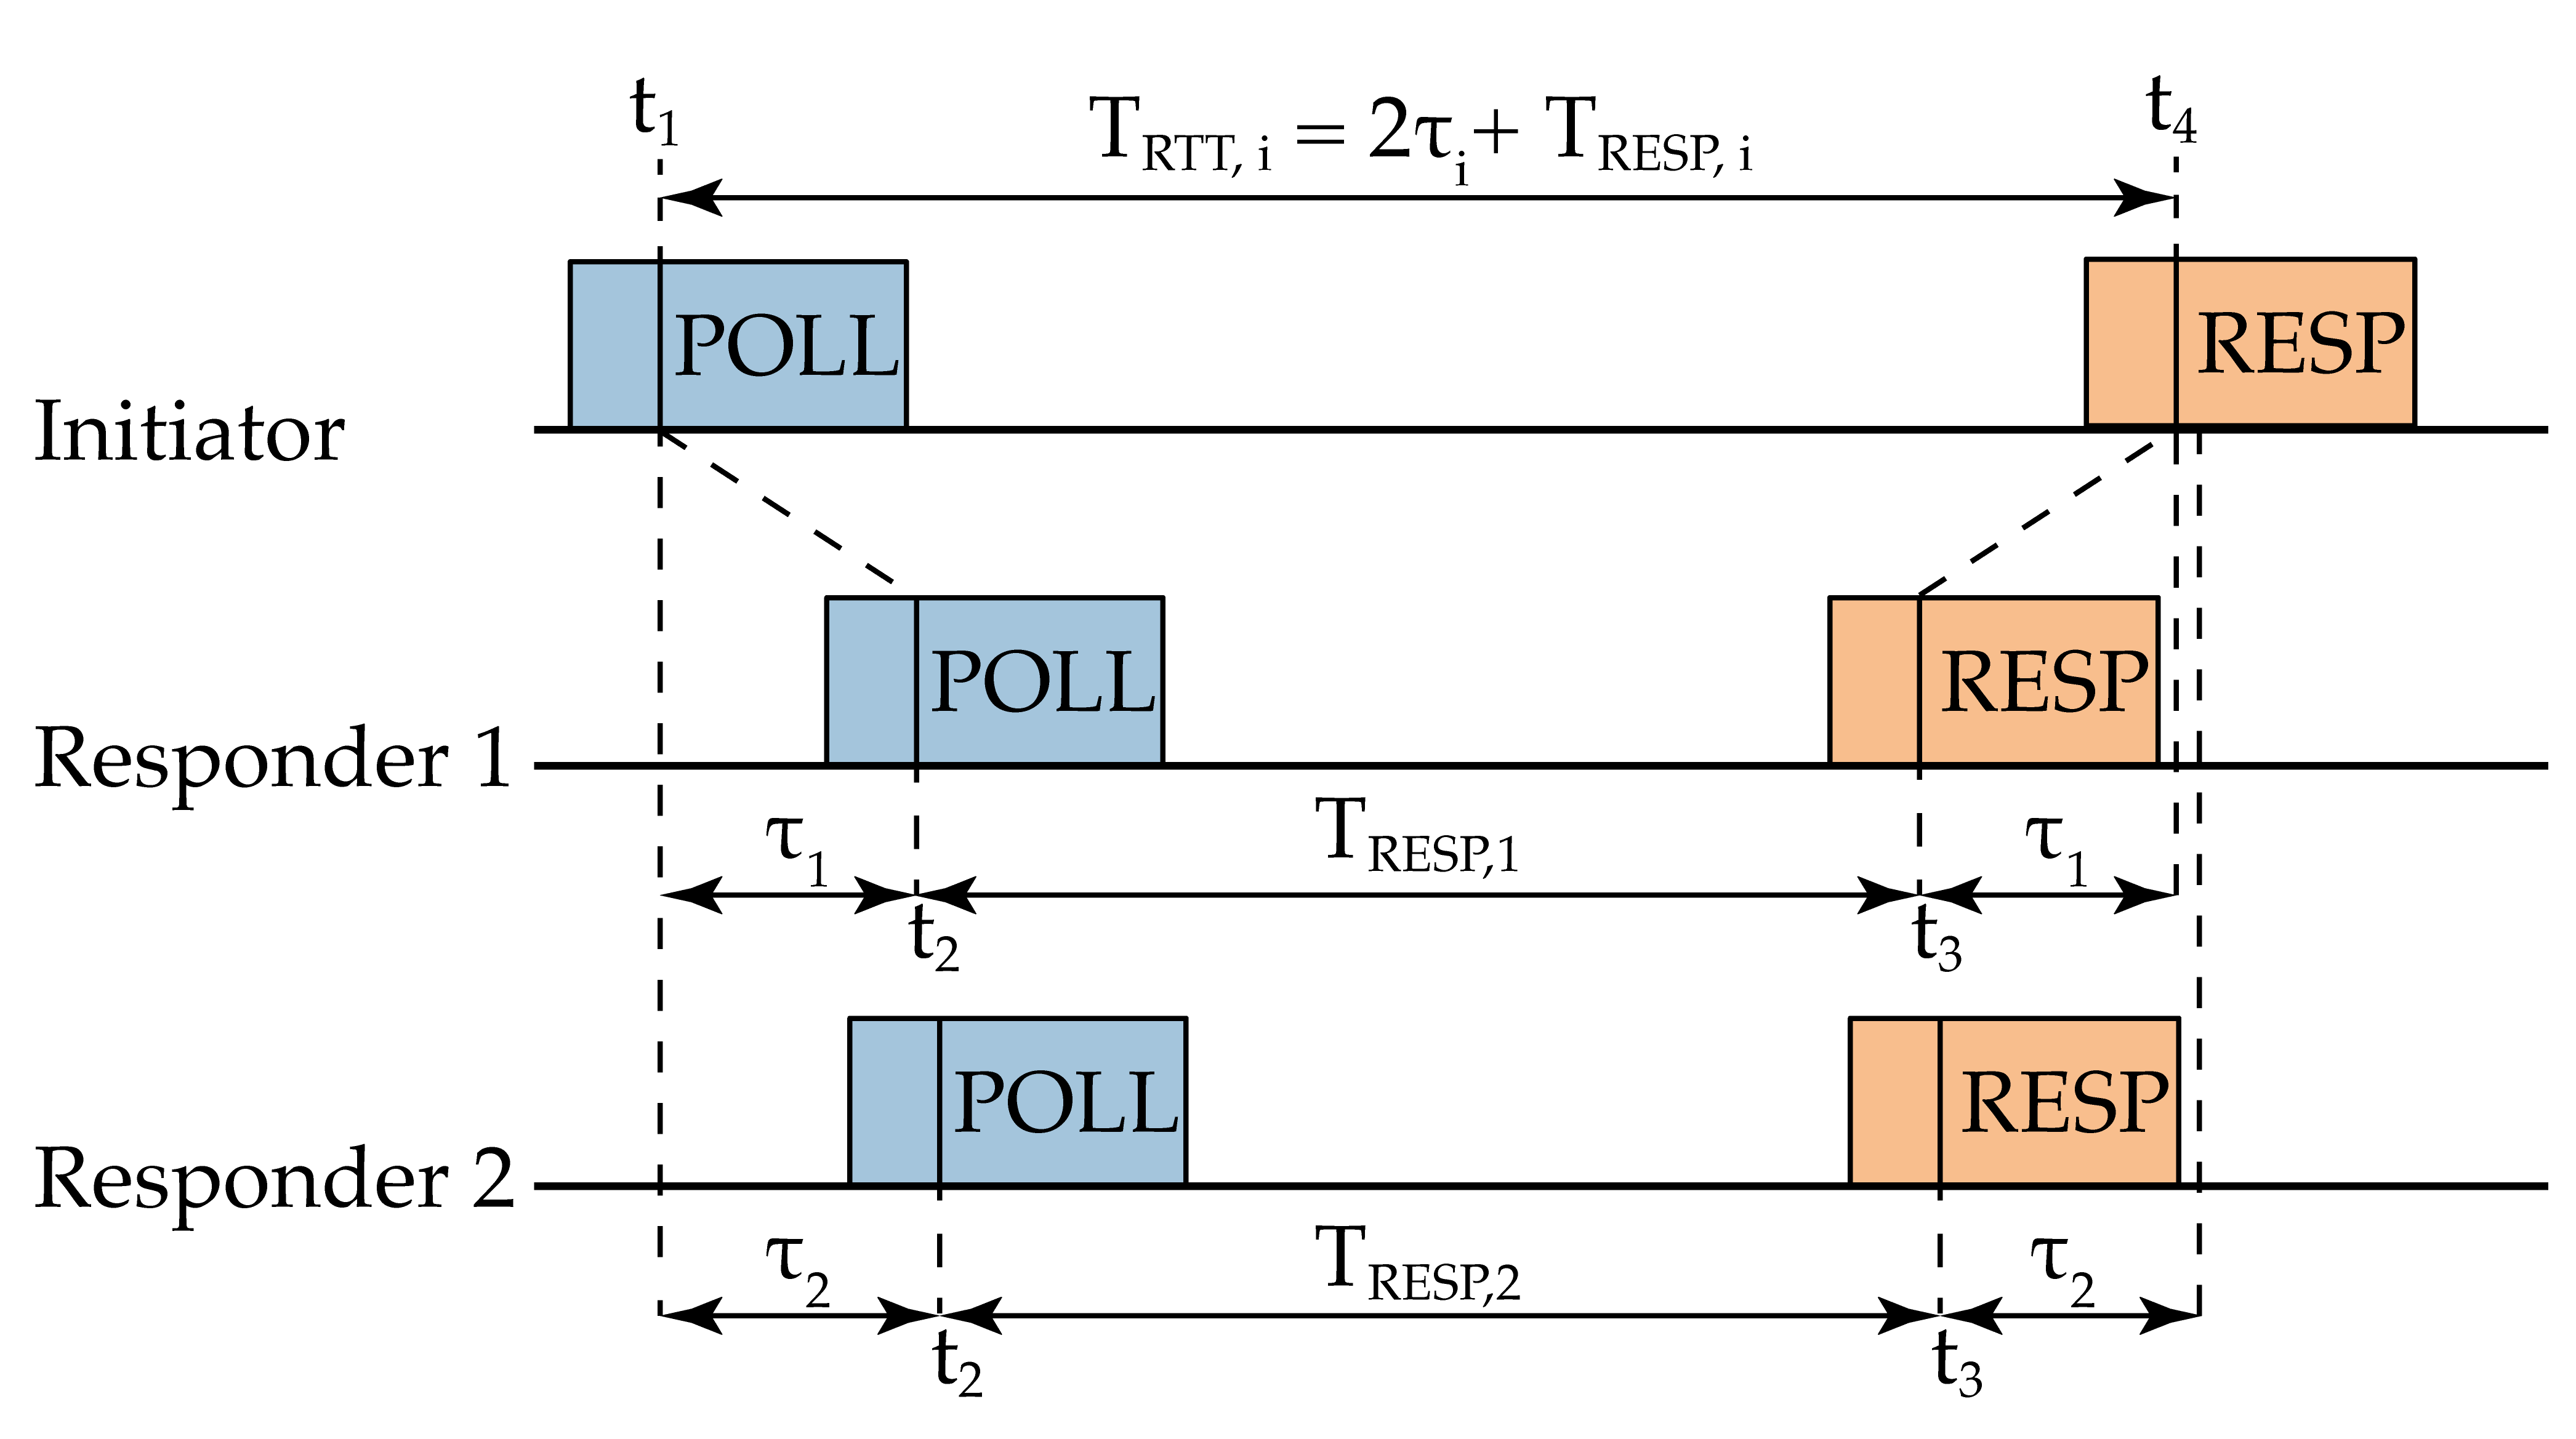
\includegraphics[width=0.55\textwidth]{image/section3/concurrent_ranging.png}
    \caption[Nguyên lý đo khoảng cách đồng thời (Concurrent Ranging)]{Nguyên lý đo khoảng cách đồng thời (Concurrent Ranging): bộ khởi tạo phát một gói poll quảng bá duy nhất, các responder phản hồi chồng lấn theo thời gian; các đường truyền được phân biệt qua đáp ứng xung kênh truyền (CIR). (\textbf{Nguồn:} Corbalán \& Picco, 2020 \cite{corbalan2020concurrent})}
    \label{fig:concurrent_ranging}
\end{figure}

\par\vspace{0.5em}
\textbf{Liên hệ với đề tài:}
\par\vspace{0.3em}
Đo khoảng cách đồng thời mở ra một hướng tối ưu quan trọng cho kiến trúc định vị đa mỏ neo của đề tài: nếu loại bỏ được nhu cầu giải mã từng gói phản hồi riêng lẻ và chỉ dựa vào CIR (vốn được vi mạch DW1000/DW3000 cung cấp sẵn cho tầng ứng dụng), chi phí mạng và năng lượng của một vòng đo $N$ mỏ neo có thể giảm đáng kể, đồng thời tăng tần suất cập nhật vị trí. Tuy nhiên, kỹ thuật này đặt ra các thách thức về độ chính xác lập lịch phát (TX scheduling) và nhận dạng responder mà hệ thống hiện tại chưa khai thác; do đó, trong phạm vi đề tài, nhóm lựa chọn chế độ DS-TWR multicast chuẩn FiRa (các responder trả lời tuần tự theo khe thời gian) để đảm bảo độ tin cậy và khả năng tích hợp với API chuẩn của hệ điều hành, đồng thời ghi nhận concurrent ranging như một định hướng nâng cấp tiềm năng trong tương lai.




%----------------------------------------------------------------------------------------------------




\subsubsection{Bảo mật UWB – Chống tấn công chuyển tiếp (Relay Attack)}

UWB là công nghệ truyền thông không dây hiếm hoi có khả năng \textbf{chống relay attack một cách hiệu quả} nhờ tận dụng các đặc tính bảo mật ở \textbf{lớp vật lý} (\textit{Physical layer security}).
\par\vspace{0.5em}
\textbf{1. Đo khoảng cách an toàn (Secure Ranging):}
\par\vspace{0.3em}
Chuẩn IEEE 802.15.4z giới thiệu cơ chế \textbf{UWB tốc độ cao} (High-Rate Pulse repetition – HRP) kết hợp với \textbf{chuỗi dấu thời gian xáo trộn} (Scrambled Timestamp Sequence – STS) nhằm ngăn chặn các cuộc tấn công chuyển tiếp và gây nhiễu \cite{ieee802154z}:

\begin{itemize}
    \item \textbf{STS:} Mỗi gói tin UWB chứa một chuỗi tiền tố (\textit{Preamble}) được xáo trộn và sinh ra từ khóa bí mật dùng chung. Kẻ tấn công không thể tự tạo hoặc chuyển tiếp một STS hợp lệ nếu không biết khóa.
    
    \item \textbf{Toàn vẹn dấu thời gian (Timestamp integrity):} Dấu thời gian đo khoảng cách được ràng buộc mật mã với nội dung gói tin, giúp phát hiện các hành vi thao túng thời gian truyền.
\end{itemize}
\par\vspace{0.5em}
\textbf{2. Các ràng buộc ở lớp vật lý:}
\par\vspace{0.3em}
\begin{itemize}
    \item \textbf{Giới hạn tốc độ ánh sáng:} Tín hiệu vô tuyến không thể truyền nhanh hơn vận tốc ánh sáng $c = 3 \times 10^8$ m/s. Nếu khoảng cách đo được nhỏ hơn khoảng cách vật lý thực tế, hệ thống có thể phát hiện hành vi relay.
    
    \item \textbf{Độ trễ rất thấp:} Quá trình đo khoảng cách bằng UWB có độ trễ nhỏ hơn 1 ms. Tấn công relay bắt buộc phải thêm độ trễ do xử lý và truyền lại tín hiệu, từ đó dễ bị phát hiện.
    
    \item \textbf{Khả năng chống đa đường truyền (Multipath resilience):} Các xung UWB cực ngắn cho phép phân biệt rõ đường truyền trực tiếp và các tín hiệu phản xạ, khiến việc giả mạo hoặc đánh lừa hệ thống trở nên rất khó khăn.
\end{itemize}

\subsubsection{Ứng dụng trong lĩnh vực ô tô}

Công nghệ UWB hiện đang được nhiều hãng ô tô lớn triển khai trong các hệ thống \textbf{chìa khóa kỹ thuật số} (Digital Key) nhờ khả năng đo khoảng cách chính xác và chống tấn công chuyển tiếp hiệu quả.
\par\vspace{0.5em}
\textbf{1. BMW Digital Key Plus (2020):}
\par\vspace{0.3em}
BMW ứng dụng công nghệ UWB sử dụng các chip dòng Trimension của NXP để thực hiện đo khoảng cách an toàn và xác định hướng tiếp cận của người dùng. Hệ thống cho phép mở khóa xe tự động khi người dùng đến gần mà không cần thao tác trên điện thoại, hay còn gọi là chế độ vào xe thụ động (\textit{Passive entry}).
\par\vspace{0.5em}
\textbf{2. Apple Car Key (iOS 14 trở lên):}
\par\vspace{0.3em}
Apple tích hợp UWB trên các thiết bị iPhone từ thế hệ iPhone 11 trở lên thông qua chip U1. Giải pháp này tuân theo chuẩn Digital Key Release 3.0 do Car Connectivity Consortium ban hành, cho phép xác thực và mở khóa xe với độ bảo mật cao.
\par\vspace{0.5em}
\textbf{3. Liên minh FiRa (FiRa Consortium):}
\par\vspace{0.3em}
FiRa Consortium là liên minh gồm nhiều tập đoàn công nghệ và ô tô lớn như Apple, Samsung, Google, BMW, Volkswagen, NXP và Qorvo, với mục tiêu xây dựng và chuẩn hóa công nghệ UWB cho các ứng dụng trong lĩnh vực ô tô, nhà thông minh và Internet vạn vật công nghiệp (Industrial IoT).

\begin{figure}[H]
    \centering
    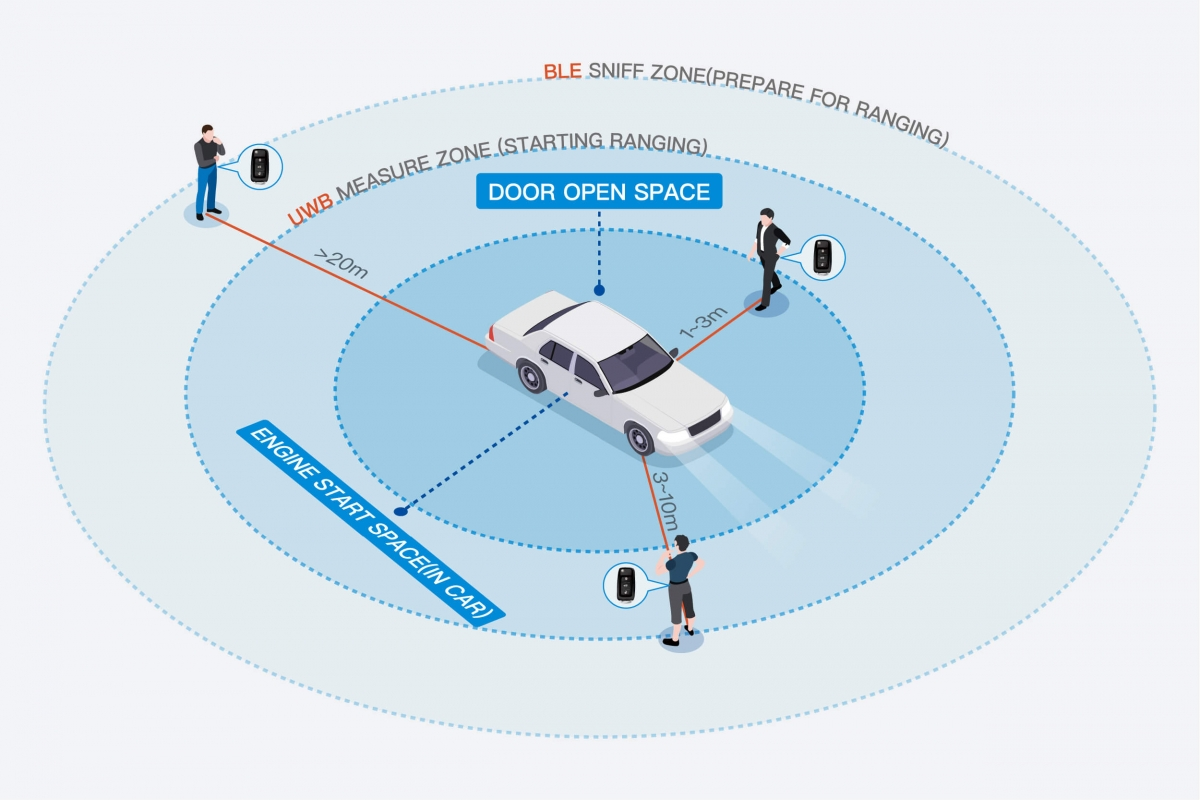
\includegraphics[width=0.8\textwidth]{image/section3/uwb4.jpg} 
    \caption[Vai trò của UWB trong hệ thống Digital Key]{Vai trò của UWB trong hệ thống Digital Key (\textbf{Nguồn:} \href{https://www.tsingcar.cn/en/business/}{TsingCar})}
    \label{fig:uwb_role}
\end{figure}



\subsection{Định vị đa mỏ neo và Trilateration}

\subsubsection{Giới hạn của kiến trúc đo khoảng cách đơn mỏ neo}

Trong giai đoạn một (Stage 1), hệ thống chỉ sử dụng duy nhất một mỏ neo (single anchor) UWB và do đó chỉ trích xuất được một giá trị khoảng cách vô hướng $d$ giữa điện thoại và xe. Về mặt hình học, một phép đo khoảng cách đơn lẻ chỉ cho biết thiết bị nằm đâu đó trên một \textbf{đường tròn} (trong không gian hai chiều) hoặc một \textbf{mặt cầu} (trong không gian ba chiều) bán kính $d$ bao quanh mỏ neo, mà không cung cấp bất kỳ thông tin nào về \textbf{hướng} (bearing) của thiết bị. Hệ quả trực tiếp là: hệ thống chỉ có thể trả lời câu hỏi \textit{``người dùng đang ở xa hay gần xe?''} (khoảng cách, 1D) mà không thể trả lời câu hỏi \textit{``người dùng đang đứng ở vị trí nào quanh xe?''} (tọa độ, 2D/3D).

Hạn chế này dẫn đến hai bất cập lớn đối với một hệ thống Smart Car Access thực thụ:
\begin{itemize}
    \item \textbf{Không thể định vị cục bộ:} Hệ thống không phân biệt được người dùng đang tiến về phía \textbf{cửa tài xế}, \textbf{cốp xe} hay \textbf{cửa phụ}, do đó không thể kích hoạt các chức năng mở khóa theo vùng (zone-based actuation) như ``mở cửa tài xế khi người dùng đến gần cột B bên trái'' hay ``mở cốp thông minh khi người dùng đứng sau đuôi xe''.
    \item \textbf{Nhạy cảm với nhiễu biên:} Quyết định mở khóa chỉ dựa trên một ngưỡng khoảng cách vô hướng ($d \le 2.0$m) rất dễ bị tác động bởi nhiễu đa đường (multipath) và nhiễu phi tuyến (NLOS), vì không có thông tin hình học nào để kiểm chứng chéo tính nhất quán của phép đo.
\end{itemize}

Để giải quyết triệt để bài toán trên, giai đoạn hai (Stage 2) nâng cấp hệ thống lên kiến trúc \textbf{định vị đa mỏ neo} (multi-anchor localization): bố trí \textbf{ba mỏ neo UWB} cố định trên thân xe, thu thập đồng thời ba khoảng cách $d_0, d_1, d_2$ và thực hiện \textbf{Trilateration} để giải ra tọa độ phẳng $(x, y)$ của thiết bị trong hệ quy chiếu gắn với xe, sau đó hợp nhất quỹ đạo bằng \textbf{Bộ lọc Kalman} hai chiều để ước lượng cả vị trí lẫn vận tốc $(x, y, v_x, v_y)$.

\subsubsection{Nguyên lý Trilateration}

Trilateration là kỹ thuật định vị dựa trên việc giao cắt các mặt hình học khoảng cách. Xét một tập $n$ mỏ neo có tọa độ đã biết $\mathbf{a}_i = (x_i, y_i)$ (trong hệ quy chiếu xe) và thiết bị cần định vị có tọa độ chưa biết $\mathbf{p} = (x, y)$. Khoảng cách đo được từ thiết bị đến mỏ neo thứ $i$ là $d_i$. Với giả thiết các mỏ neo và thiết bị cùng nằm trên một mặt phẳng ngang (độ cao xấp xỉ bằng nhau), ta có hệ phương trình phi tuyến:

\begin{equation}
    \lVert \mathbf{p} - \mathbf{a}_i \rVert = \sqrt{(x - x_i)^2 + (y - y_i)^2} = d_i, \qquad i = 0, 1, \dots, n-1
\end{equation}

Ý nghĩa hình học của từng phương trình:
\begin{itemize}
    \item \textbf{Một mỏ neo:} Tập nghiệm là một đường tròn tâm $\mathbf{a}_0$ bán kính $d_0$ --- vô số vị trí khả dĩ (bài toán 1D, không xác định được hướng).
    \item \textbf{Hai mỏ neo:} Giao của hai đường tròn cho tối đa \textbf{hai} nghiệm đối xứng nhau qua đoạn thẳng nối hai tâm --- bài toán vẫn còn tính lưỡng trị (ambiguity).
    \item \textbf{Ba mỏ neo (không thẳng hàng):} Giao của ba đường tròn xác định \textbf{duy nhất một điểm} trên mặt phẳng --- đây là cấu hình tối thiểu để định vị 2D không lưỡng trị.
\end{itemize}

\begin{figure}[H]
    \centering
    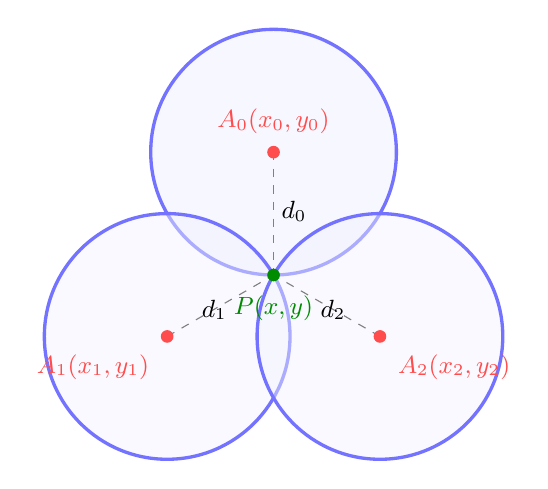
\begin{tikzpicture}[scale=0.52, every node/.style={font=\small}]
        \coordinate (A0) at (0,3.0);
        \coordinate (A1) at (-2.598,-1.5);
        \coordinate (A2) at (2.598,-1.5);
        \coordinate (P)  at (0,0);

        \draw[blue!55, very thick, fill=blue!6, fill opacity=0.55] (A0) circle (3.0);
        \draw[blue!55, very thick, fill=blue!5, fill opacity=0.45] (A1) circle (3.0);
        \draw[blue!55, very thick, fill=blue!5, fill opacity=0.45] (A2) circle (3.0);

        \draw[dashed, gray] (A0) -- (P);
        \draw[dashed, gray] (A1) -- (P);
        \draw[dashed, gray] (A2) -- (P);

        \filldraw[red!70] (A0) circle (4pt) node[above=3pt] {$A_0(x_0,y_0)$};
        \filldraw[red!70] (A1) circle (4pt) node[below left=3pt] {$A_1(x_1,y_1)$};
        \filldraw[red!70] (A2) circle (4pt) node[below right=3pt] {$A_2(x_2,y_2)$};

        \node at (0.5,1.55) {$d_0$};
        \node at (-1.45,-0.85) {$d_1$};
        \node at (1.45,-0.85) {$d_2$};

        \filldraw[green!55!black] (P) circle (4pt) node[below=4pt] {$P(x,y)$};
    \end{tikzpicture}
    \caption[Nguyên lý Trilateration với ba mỏ neo]{Nguyên lý Trilateration: giao của ba đường tròn bán kính $d_0, d_1, d_2$ (tâm là ba mỏ neo $A_0, A_1, A_2$) xác định duy nhất vị trí $P(x,y)$ của thiết bị.}
    \label{fig:trilateration_principle}
\end{figure}

\textbf{Mở rộng sang không gian ba chiều:} Trong trường hợp tổng quát, mỗi phép đo $d_i$ mô tả một \textbf{mặt cầu} bán kính $d_i$ trong không gian 3D, và cần tối thiểu \textbf{bốn} mỏ neo không đồng phẳng để giải ra tọa độ $(x, y, z)$ một cách duy nhất. Trong phạm vi đề tài, các mỏ neo được gắn trên cùng một mặt phẳng ngang của thân xe và bài toán điều khiển truy cập chỉ cần đến tọa độ mặt phẳng $(x, y)$ (độ cao thiết bị cầm tay được xem là hằng số), do đó hệ ba phương trình mặt cầu được rút gọn về hệ ba phương trình đường tròn nêu trên. Công thức và thuật toán trình bày dưới đây hoàn toàn có thể mở rộng lên ba chiều bằng cách bổ sung thêm biến $z$ và ít nhất một mỏ neo thứ tư \cite{murphy1995trilateration}.

\subsubsection{Nghiệm đại số tuyến tính (Linear Least Squares)}

Để giải hệ phương trình phi tuyến trên một cách hiệu quả trên vi điều khiển, bước đầu tiên là \textbf{tuyến tính hóa} bằng phép trừ phương trình. Bình phương hai vế của từng phương trình:

\begin{equation}
    (x - x_i)^2 + (y - y_i)^2 = d_i^2
\end{equation}

Khai triển và trừ phương trình thứ $i$ cho một phương trình tham chiếu (chọn mỏ neo $A_0$):

\begin{equation}
    -2x(x_i - x_0) - 2y(y_i - y_0) = d_i^2 - d_0^2 - (x_i^2 + y_i^2) + (x_0^2 + y_0^2)
\end{equation}

Viết lại dưới dạng ma trận $\mathbf{A}\mathbf{p} = \mathbf{b}$:

\begin{equation}
    \mathbf{A} =
    \begin{bmatrix}
        x_1 - x_0 & y_1 - y_0 \\
        x_2 - x_0 & y_2 - y_0 \\
        \vdots & \vdots \\
        x_{n-1} - x_0 & y_{n-1} - y_0
    \end{bmatrix}, \qquad
    \mathbf{b} = -\frac{1}{2}
    \begin{bmatrix}
        d_1^2 - d_0^2 - \lVert \mathbf{a}_1 \rVert^2 + \lVert \mathbf{a}_0 \rVert^2 \\
        d_2^2 - d_0^2 - \lVert \mathbf{a}_2 \rVert^2 + \lVert \mathbf{a}_0 \rVert^2 \\
        \vdots
    \end{bmatrix}
\end{equation}

Với ba mỏ neo, hệ gồm hai phương trình độc lập và hai ẩn số, giải trực tiếp bằng phép nghịch đảo. Trong trường hợp có nhiều hơn ba mỏ neo (hệ quá xác định --- overdetermined), nghiệm bình phương tối thiểu (Least Squares) được tính bằng công thức chuẩn tắc:

\begin{equation}
    \hat{\mathbf{p}} = (\mathbf{A}^T \mathbf{A})^{-1} \mathbf{A}^T \mathbf{b}
\end{equation}

Nghiệm đại số này đóng vai trò \textbf{hạt giống khởi tạo} (initial seed) cho bước tối ưu phi tuyến bên dưới, giúp vòng lặp hội tụ nhanh và tránh rơi vào cực tiểu cục bộ sai.

\subsubsection{Trường hợp hai mỏ neo và sự lưỡng trị}

Khi chỉ có hai mỏ neo hợp lệ (ví dụ một mỏ neo bị mất gói tin hoặc nhiễu nặng), giao của hai đường tròn cho hai nghiệm đối xứng. Đặt $D = \lVert \mathbf{a}_1 - \mathbf{a}_0 \rVert$ là khoảng cách giữa hai tâm. Tồn tại nghiệm khi và chỉ khi bất đẳng thức tam giác được thỏa mãn: $|d_0 - d_1| \le D \le d_0 + d_1$. Khi đó:
\begin{itemize}
    \item \textbf{Nếu $D = d_0 + d_1$ hoặc $D = |d_0 - d_1|$:} Hai đường tròn tiếp xúc tại đúng một điểm.
    \item \textbf{Nếu các đường tròn không giao nhau (do nhiễu):} Thuật toán suy biến về điểm nằm trên đoạn thẳng nối hai tâm, tỷ lệ theo trọng số khoảng cách, đảm bảo luôn trả về một ước lượng hợp lý thay vì báo lỗi.
\end{itemize}

Trong hệ thống thực tế, hai nghiệm lưỡng trị được giải quyết bằng cách dùng \textbf{ước lượng vị trí của chu kỳ trước} (do bộ lọc Kalman duy trì) làm tham chiếu để chọn nghiệm gần nhất, hoặc bỏ qua khung dữ liệu đó nếu độ tin cậy thấp.

\subsubsection{Phương pháp Gauss-Newton}

Nghiệm tuyến tính hóa ở trên bỏ qua thành phần bậc hai nên có thể thiếu chính xác khi nhiễu lớn. Do đó, hệ thống sử dụng thêm một vòng lặp \textbf{Gauss-Newton} để tối ưu phi tuyến. Định nghĩa vector thặng dư (residual):

\begin{equation}
    \mathbf{r}(\mathbf{p}) =
    \begin{bmatrix}
        \lVert \mathbf{p} - \mathbf{a}_0 \rVert - d_0 \\
        \lVert \mathbf{p} - \mathbf{a}_1 \rVert - d_1 \\
        \lVert \mathbf{p} - \mathbf{a}_2 \rVert - d_2
    \end{bmatrix}
\end{equation}

Mục tiêu là cực tiểu hóa hàm chi phí bình phương tối thiểu phi tuyến $f(\mathbf{p}) = \tfrac{1}{2} \lVert \mathbf{r}(\mathbf{p}) \rVert^2$. Ma trận Jacobian của vector thặng dư theo $\mathbf{p}$:

\begin{equation}
    \mathbf{J}(\mathbf{p}) =
    \begin{bmatrix}
        \dfrac{x - x_0}{\lVert \mathbf{p} - \mathbf{a}_0 \rVert} & \dfrac{y - y_0}{\lVert \mathbf{p} - \mathbf{a}_0 \rVert} \\[1.2em]
        \dfrac{x - x_1}{\lVert \mathbf{p} - \mathbf{a}_1 \rVert} & \dfrac{y - y_1}{\lVert \mathbf{p} - \mathbf{a}_1 \rVert} \\[1.2em]
        \dfrac{x - x_2}{\lVert \mathbf{p} - \mathbf{a}_2 \rVert} & \dfrac{y - y_2}{\lVert \mathbf{p} - \mathbf{a}_2 \rVert}
    \end{bmatrix}
\end{equation}

Mỗi bước lặp cập nhật nghiệm theo phương trình chuẩn tắc:

\begin{equation}
    \mathbf{p}^{(k+1)} = \mathbf{p}^{(k)} - \left(\mathbf{J}^T \mathbf{J}\right)^{-1} \mathbf{J}^T\, \mathbf{r}(\mathbf{p}^{(k)})
\end{equation}

Vòng lặp kết thúc khi bước dịch chuyển nhỏ hơn ngưỡng hội tụ hoặc đạt số lần lặp tối đa (trong đề tài giới hạn 10 vòng). Điểm khởi tạo $\mathbf{p}^{(0)}$ được lấy từ nghiệm tuyến tính ở trên hoặc từ vị trí ước lượng của chu kỳ trước. Bên cạnh tọa độ, thuật toán còn trả về \textbf{giá trị RMS của thặng dư}:

\begin{equation}
    \text{RMS} = \sqrt{\frac{1}{n}\sum_{i=0}^{n-1} \left(\lVert \hat{\mathbf{p}} - \mathbf{a}_i \rVert - d_i\right)^2}
\end{equation}

Đại lượng RMS này là một thước đo \textbf{chất lượng lời giải} (fix quality): RMS nhỏ cho thấy ba khoảng cách nhất quán về mặt hình học, trong khi RMS lớn là dấu hiệu của nhiễu đa đường, che khuất tầm nhìn (NLOS) hoặc dữ liệu nhiễu. Giá trị này được nạp trực tiếp vào ma trận hiệp phương sai nhiễu đo $R$ của bộ lọc Kalman ở mục tiếp theo, giúp bộ lọc \textbf{tự động giảm mức tin cậy} đối với các khung dữ liệu kém chất lượng.

\subsubsection{Độ suy giảm chính xác hình học (GDOP)}

Độ chính xác của kết quả định vị không chỉ phụ thuộc vào nhiễu của phép đo khoảng cách mà còn phụ thuộc mạnh vào \textbf{hình học bố trí} của các mỏ neo. Mối quan hệ này được lượng hóa bằng chỉ số \textbf{Geometric Dilution of Precision (GDOP)} \cite{langley1999gdop}: cùng một mức nhiễu khoảng cách, nếu các mỏ neo bố trí gần như thẳng hàng hoặc cụm sát nhau, sai số vị trí sẽ bị \textbf{khuếch đại} lên rất lớn, đặc biệt tại các vùng nằm xa tam giác mỏ neo. Ngược lại, một cấu hình tam giác bao trùm vùng hoạt động sẽ cho GDOP thấp và sai số được kiểm soát \cite{ridolfi2018analysis}.

Trong đề tài, ba mỏ neo được bố trí theo một tam giác không thẳng hàng ôm lấy thân xe (Hình \ref{fig:anchor_geometry}): $A_0$ ở trung tâm cản sau, $A_1$ ở bên phải thân xe và $A_2$ ở cột B bên trái (đồng thời là điểm mở khóa cửa tài xế). Cấu hình này đảm bảo GDOP thấp ngay tại vùng cửa tài xế --- vùng quyết định mở khóa quan trọng nhất --- đồng thời hạn chế sai số tại vùng cốp xe.

\begin{figure}[H]
    \centering
    \begin{tikzpicture}[scale=0.72, every node/.style={font=\small}]
        % Car body (X right, Y forward)
        \draw[fill=gray!12, thick] (-1.0,-2.0) rectangle (1.0,2.0);
        \node[gray!70] at (0,0.0) {\textit{Thân xe}};

        % Coordinate axes
        \draw[->, thick] (0,-2.6) -- (0,2.9) node[above] {$y$ (tiến)};
        \draw[->, thick] (-1.7,0) -- (1.6,0) node[right] {$x$ (phải)};

        % Anchors
        \filldraw[red!70] (0,-2.0)  circle (3.5pt) node[below=3pt] {$A_0\,(0,\,-2.0)$};
        \filldraw[red!70] (0.95,0)  circle (3.5pt) node[right=3pt] {$A_1\,(0.95,\,0)$};
        \filldraw[red!70] (-0.95,0) circle (3.5pt) node[left=3pt]  {$A_2\,(-0.95,\,0)$};

        % Unlock point (driver door B-pillar = A2)
        \filldraw[green!55!black] (-0.95,0) circle (3.5pt);
        \node[green!45!black, right=3pt, align=left] at (-0.95,0.15) {Điểm mở khóa\\ (cửa tài xế)};
    \end{tikzpicture}
    \caption[Hệ tọa độ xe và bố trí ba mỏ neo UWB]{Hệ tọa độ gắn với xe và bố trí ba mỏ neo UWB: $A_0$ (trung tâm cản sau), $A_1$ (bên phải thân xe), $A_2$ (cột B bên trái --- đồng thời là điểm mở khóa cửa tài xế). Đơn vị: mét.}
    \label{fig:anchor_geometry}
\end{figure}

\subsection{Bộ lọc Kalman hai chiều (EKF) cho bám quỹ đạo}

Dữ liệu tọa độ $(x, y)$ thu được từ Trilateration vẫn chứa các thành phần nhiễu trắng và nhiễu do hiện tượng phản xạ đa đường (multipath), đặc biệt là các ``bước nhảy'' vị trí khi tín hiệu bị che khuất (NLOS). Nếu sử dụng trực tiếp kết quả thô, hệ thống sẽ gặp hiện tượng dao động (chattering) khi ra quyết định mở cửa. Bộ lọc Kalman --- được phát triển bởi Rudolf E. Kalman năm 1960 \cite{kalman1960} --- là một thuật toán ước lượng trạng thái tối ưu theo đệ quy cho các hệ thống tuyến tính chịu tác động của nhiễu Gauss \cite{welch2001kalman}. Trong đề tài, bộ lọc được sử dụng để \textbf{hợp nhất} chuỗi tọa độ đo từ Trilateration thành quỹ đạo mượt, đồng thời ước lượng cả vector vận tốc $(v_x, v_y)$ phục vụ cho cổng logic hướng tiếp cận (approach gate) ở tầng quyết định truy cập.

\textbf{Lưu ý về tính phi tuyến:} Phép đo khoảng cách $\rightarrow$ tọa độ vốn là bài toán phi tuyến, nhưng phần phi tuyến đã được xử lý triệt để ngay tại tầng Trilateration (Gauss-Newton). Do đó, tầng lọc chỉ làm việc với quan hệ đo tuyến tính $z = Hx + v$ và mô hình vận tốc hằng tuyến tính; bộ lọc Kalman mở rộng (Extended Kalman Filter) trong trường hợp này suy biến về đúng bộ lọc Kalman tuyến tính chuẩn.

\subsubsection{Mô hình trạng thái}

Vector trạng thái gồm bốn thành phần:

\begin{equation}
    \mathbf{x}_k = \begin{bmatrix} p_x & p_y & v_x & v_y \end{bmatrix}^T
\end{equation}

trong đó $(p_x, p_y)$ là vị trí (mét) và $(v_x, v_y)$ là vận tốc (mét/giây) của thiết bị trong hệ quy chiếu xe. Giả thiết chuyển động của người đi bộ được mô tả bởi mô hình \textbf{vận tốc hằng} (constant velocity) với nhiễu gia tốc ngẫu nhiên (manoeuvre noise):

\begin{equation}
    \mathbf{x}_{k} = \mathbf{F}(\Delta t)\, \mathbf{x}_{k-1} + \mathbf{w}_{k-1}, \qquad
    \mathbf{F}(\Delta t) =
    \begin{bmatrix}
        1 & 0 & \Delta t & 0 \\
        0 & 1 & 0 & \Delta t \\
        0 & 0 & 1 & 0 \\
        0 & 0 & 0 & 1
    \end{bmatrix}
\end{equation}

với $\Delta t$ là khoảng thời gian giữa hai chu kỳ xử lý, $\mathbf{w} \sim \mathcal{N}(0, \mathbf{Q})$ là nhiễu quá trình. Sử dụng mô hình nhiễu gia tốc trắng liên tục với cường độ $\sigma_a$, ma trận hiệp phương sai nhiễu quá trình có dạng:

\begin{equation}
    \mathbf{Q} = \sigma_a^2
    \begin{bmatrix}
        \tfrac{\Delta t^4}{4} & 0 & \tfrac{\Delta t^3}{2} & 0 \\[0.3em]
        0 & \tfrac{\Delta t^4}{4} & 0 & \tfrac{\Delta t^3}{2} \\[0.3em]
        \tfrac{\Delta t^3}{2} & 0 & \Delta t^2 & 0 \\[0.3em]
        0 & \tfrac{\Delta t^3}{2} & 0 & \Delta t^2
    \end{bmatrix}
\end{equation}

\subsubsection{Mô hình đo lường}

Phép đo ở mỗi chu kỳ là tọa độ $(x_{meas}, y_{meas})$ do Trilateration trả về:

\begin{equation}
    \mathbf{z}_k = \begin{bmatrix} x_{meas} \\ y_{meas} \end{bmatrix} = \mathbf{H}\, \mathbf{x}_k + \mathbf{v}_k, \qquad
    \mathbf{H} = \begin{bmatrix} 1 & 0 & 0 & 0 \\ 0 & 1 & 0 & 0 \end{bmatrix}, \qquad \mathbf{v} \sim \mathcal{N}(0, \mathbf{R})
\end{equation}

Ma trận hiệp phương sai nhiễu đo được xây dựng từ chất lượng lời giải Trilateration:

\begin{equation}
    \mathbf{R} = \sigma_{meas}^2 \, \mathbf{I}_{2\times 2}, \qquad
    \sigma_{meas} = \operatorname{clamp}(\text{RMS},\; 0.05,\; 1.0)
\end{equation}

Việc ràng buộc $\sigma_{meas}$ trong khoảng $[0.05,\,1.0]$ m đảm bảo bộ lọc không bao giờ tin tưởng mù quáng một khung dữ liệu ``quá tốt'' (nhiều khả năng là ngẫu nhiên) và cũng không loại bỏ hoàn toàn một khung dữ liệu nhiễu lớn.

\subsubsection{Hai giai đoạn của bộ lọc}

\paragraph*{A. Giai đoạn dự báo (Time Update / Predict)}

\begin{align}
    \hat{\mathbf{x}}_{k|k-1} &= \mathbf{F}(\Delta t)\, \hat{\mathbf{x}}_{k-1|k-1} \\
    \mathbf{P}_{k|k-1} &= \mathbf{F}\, \mathbf{P}_{k-1|k-1}\, \mathbf{F}^T + \mathbf{Q}
\end{align}

Giai đoạn dự báo được thực thi ở một nhịp cố định \textbf{10 Hz} ($\Delta t = 100$ ms), độc lập với nhịp nhận dữ liệu thô từ cầu nối (bridge). Điều này mang lại hai lợi ích: (i) đồng hồ ra quyết định mở khóa được giữ ổn định; (ii) khi một vài khung dữ liệu bị mất (dropped frames), bộ lọc vẫn \textbf{dự báo bù} (coasting) để lấp đầy khoảng trống quỹ đạo, miễn là khoảng trống không vượt quá ngưỡng cho phép (trong đề tài là 2 giây; nếu quá ngưỡng, quỹ đạo được khởi tạo lại từ đầu).

\paragraph*{B. Giai đoạn cập nhật (Measurement Update / Correct)}

Khi nhận được phép đo mới $\mathbf{z}_k$, bộ lọc tính toán:
\begin{itemize}
    \item \textbf{Vector đổi mới (Innovation):}
    \begin{equation}
        \tilde{\mathbf{y}}_k = \mathbf{z}_k - \mathbf{H}\, \hat{\mathbf{x}}_{k|k-1}
    \end{equation}
    \item \textbf{Ma trận hiệp phương sai đổi mới:}
    \begin{equation}
        \mathbf{S}_k = \mathbf{H}\, \mathbf{P}_{k|k-1}\, \mathbf{H}^T + \mathbf{R}
    \end{equation}
    \item \textbf{Độ lợi Kalman (Kalman Gain):}
    \begin{equation}
        \mathbf{K}_k = \mathbf{P}_{k|k-1}\, \mathbf{H}^T\, \mathbf{S}_k^{-1}
    \end{equation}
    \item \textbf{Cập nhật trạng thái ước lượng:}
    \begin{equation}
        \hat{\mathbf{x}}_{k|k} = \hat{\mathbf{x}}_{k|k-1} + \mathbf{K}_k\, \tilde{\mathbf{y}}_k
    \end{equation}
    \item \textbf{Cập nhật hiệp phương sai sai số:}
    \begin{equation}
        \mathbf{P}_{k|k} = (\mathbf{I} - \mathbf{K}_k\, \mathbf{H})\, \mathbf{P}_{k|k-1}
    \end{equation}
\end{itemize}

\paragraph*{C. Cổng lọc đổi mới (Innovation Gating)}

Để chống lại các xung nhiễu NLOS/multipath khiến tọa độ đo bị ``nhảy vọt'' xa khỏi quỹ đạo dự báo, bộ lọc áp dụng cơ chế \textbf{lọc ngưỡng đổi mới} (innovation gating): nếu chuẩn của vector đổi mới vượt quá bội số $k$ của độ lệch chuẩn dự báo ($\lVert \tilde{\mathbf{y}}_k \rVert > k\, \sqrt{\operatorname{tr}(\mathbf{S}_k)}$), phép đo được hạ cấp hoặc bỏ qua trong chu kỳ đó. Cơ chế này giúp quỹ đạo bám mượt ngay cả khi người dùng đi qua vùng che khuất, đồng thời vẫn giữ được phản hồi nhanh khi chuyển động là hợp lý.

\subsubsection{Cấu hình tham số thực nghiệm}

Hiệu quả của bộ lọc phụ thuộc vào việc cân bằng giữa hai ma trận $\mathbf{Q}$ (nhiễu quá trình) và $\mathbf{R}$ (nhiễu đo). Trong thực nghiệm triển khai trên ESP32-S3, cường độ nhiễu gia tốc được chọn $\sigma_a = 1.2$ m/s$^2$ --- đủ lớn để bộ lọc bám theo sự đổi hướng đột ngột của người đi bộ, nhưng đủ nhỏ để làm mượt nhiễu đo:
\begin{itemize}
    \item Nếu chọn $\mathbf{Q}$ lớn và $\mathbf{R}$ nhỏ: Bộ lọc tin vào cảm biến hơn, đáp ứng nhanh với thay đổi nhưng quỹ đạo bị nhiễu và dễ bị kéo lệch bởi xung NLOS.
    \item Nếu chọn $\mathbf{Q}$ nhỏ và $\mathbf{R}$ lớn: Bộ lọc tin vào mô hình chuyển động hơn, quỹ đạo rất mượt nhưng trễ (lag) so với bước đi thực tế và phản ứng chậm khi người dùng đổi hướng.
\end{itemize}

Dựa trên đặc tính chuyển động của con người (tốc độ đi bộ $\approx 1.2$ m/s) và nhịp xử lý 10Hz, bộ tham số trên đã được tinh chỉnh để quỹ đạo $(x, y)$ và vận tốc $(v_x, v_y)$ vừa mượt mà vừa phản hồi kịp thời, làm đầu vào cho tầng quyết định truy cập hình học (geometric access control) ở giai đoạn hai.



\subsection{Triển khai UWB – Phần cứng trong hệ thống}

\textbf{Trong đề tài này:} Công nghệ UWB đã được \textbf{hiện thực hóa hoàn toàn} và đóng vai trò là chốt chặn bảo mật vật lý cốt lõi của hệ thống. Sự kết hợp giữa vi điều khiển ESP32-S3 và \textbf{ba mỏ neo UWB} (sử dụng vi mạch tiêu chuẩn DW3000) giúp hệ thống đo lường khoảng cách theo thời gian thực (Real-time Secure Ranging), đồng thời hợp nhất ba khoảng cách thành tọa độ phẳng $(x, y)$ để định vị không gian (Real-time Localization).

Việc triển khai UWB thực tế giải quyết triệt để các hạn chế của bảo mật BLE thông thường:
\begin{itemize}
    \item \textbf{Đo khoảng cách chính xác (ToF):} Xác minh người dùng đang thực sự ở cạnh xe (với sai số chỉ ở mức centimet) thay vì chỉ dựa vào cường độ tín hiệu RSSI vốn dễ bị làm giả.
    \item \textbf{Định vị đa mỏ neo (Trilateration):} Xác định vị trí tương đối $(x, y)$ của người dùng quanh xe, làm nền tảng cho việc kích hoạt mở khóa theo vùng (cửa tài xế, cốp xe) thay vì chỉ so sánh một ngưỡng khoảng cách đơn lẻ.
    \item \textbf{Bảo vệ bằng STS (Scrambled Timestamp Sequence):} Kích hoạt cơ chế mã hóa xung UWB ở lớp vật lý, giúp loại bỏ hoàn toàn rủi ro tấn công tiếp sóng (Relay Attack).
\end{itemize}

\begin{table}[h]
\centering
\label{tab:uwb_chips}
\begin{tabular}{|l|l|l|l|}
\hline
\textbf{Vi mạch} & \textbf{Nhà sản xuất} & \textbf{Chuẩn IEEE} & \textbf{Ứng dụng trong đề tài} \\
\hline
DW3000 & Qorvo (Decawave) & 802.15.4a/z & Vi mạch thu phát cho ba mỏ neo UWB \\
SR040 / SR150 & NXP Trimension & 802.15.4z & Tham chiếu kiến trúc \\
U1 & Apple (độc quyền) & 802.15.4z & Tương tác từ phía Mobile \\
\hline
\end{tabular}
\caption{Các vi mạch UWB phổ biến và vai trò triển khai}
\end{table}

%-----------------------------------------------------------------------

\subsection{So sánh các công nghệ NFC, BLE, UWB}

Phần này trình bày so sánh tổng quan giữa ba công nghệ truyền thông không dây NFC, BLE và UWB dựa trên các tiêu chí kỹ thuật quan trọng cũng như mức độ phù hợp đối với bài toán Smart Car Access trong đề tài.

\begin{table}[h]
\centering
\label{tab:wireless_comparison}
\begin{tabular}{|l|p{3.5cm}|p{4cm}|p{4cm}|}
\hline
\textbf{Tiêu chí} & \textbf{NFC} & \textbf{BLE} & \textbf{UWB} \\
\hline
Phạm vi hoạt động & < 10 cm & 10–50 m & 10–200 m \\
\hline
Tốc độ dữ liệu & 424 kbps & 1–2 Mbps & 110 kbps – 27 Mbps \\
\hline
Thời gian kết nối & < 0.1 s & 1–2 s & < 0.5 s \\
\hline
Công suất tiêu thụ & Thẻ thụ động: 0 mW & 10–50 mW & 50–100 mW \\
\hline
Đo khoảng cách & Không hỗ trợ & RSSI (không chính xác) & ToF (±10–30 cm) \\
\hline
Cơ chế bảo mật chính & Tiếp xúc vật lý gần & Ghép nối và mã hóa & Secure ranging (STS) \\
\hline
Chống Relay attack & Cao & Thấp & Rất cao  \\
\hline
Vai trò & Cấp phát khóa & Xác thực & Bảo mật \\
\hline
Chi phí ước tính & \$1–2 & \$2–3 & \$12–15 \\
\hline
\end{tabular}
\caption{So sánh mức độ phù hợp của NFC, BLE và UWB}
\end{table}


\textbf{Kết luận:} Kiến trúc kết hợp NFC cho giai đoạn cấp phát an toàn, BLE cho sự thuận tiện trong quá trình sử dụng hằng ngày, và UWB cho khả năng chống tấn công chuyển tiếp trong tương lai mang lại một giải pháp cân bằng tối ưu giữa mức độ bảo mật, trải nghiệm người dùng và chi phí triển khai hệ thống.

\subsection{Kiến trúc Digital Key theo chuẩn Car Connectivity Consortium (CCC)}

Car Connectivity Consortium (CCC) là tổ chức công nghiệp toàn cầu chịu trách nhiệm phát triển các tiêu chuẩn cho kết nối giữa điện thoại thông minh và phương tiện giao thông. Phiên bản \textbf{CCC Digital Key Release 3.0} là một bước ngoặt lớn khi chuẩn hóa việc kết hợp đồng thời 3 công nghệ: NFC, BLE và UWB vào cùng một kiến trúc bảo mật đồng nhất. 

Đề tài được thiết kế bám sát theo kiến trúc của CCC Release 3 với sự phân công nhiệm vụ rõ ràng cho từng giao thức:
\begin{itemize}
    \item \textbf{NFC (Cơ chế dự phòng và Cấp phát):} Đóng vai trò là phương thức ghép nối ban đầu (Provisioning / Pairing) để trao đổi khóa an toàn. Ngoài ra, NFC hoạt động như phương thức mở khóa dự phòng (Fallback) khi điện thoại hết pin nhờ cơ chế Host Card Emulation (HCE).
    \item \textbf{BLE (Thiết lập kênh bảo mật - Secure Channel):} Đóng vai trò cầu nối liên lạc chính ở khoảng cách xa. BLE chịu trách nhiệm thiết lập kết nối mã hóa, xác thực danh tính hai chiều (Mutual Authentication) và trao đổi các tham số phiên làm việc cho UWB.
    \item \textbf{UWB (Xác minh khoảng cách an toàn - Secure Ranging):} Chỉ được đánh thức sau khi kênh BLE đã xác thực thành công. UWB thực hiện các phép đo thời gian bay (Time-of-Flight) có mã hóa để đảm bảo thiết bị thực sự nằm trong vùng an toàn (Secure Zone) trước khi kích hoạt lệnh mở khóa cửa xe.
\end{itemize}
Sự kết hợp này tạo ra một hệ thống "Miễn nhiễm với Relay Attack", nơi BLE xử lý logic mật mã còn UWB xác thực ranh giới vật lý.

\section{Mật mã học và bảo mật}

Hệ thống Smart Car Access Control yêu cầu các cơ chế bảo mật mạnh mẽ để đảm bảo tính toàn vẹn, bảo mật và xác thực trong quá trình truyền thông giữa điện thoại và xe. Phần này trình bày các khái niệm mật mã học được áp dụng trực tiếp trong đề tài, bao gồm mật mã đường cong Elliptic (ECC) cho Key exchange và Digital signature, mã hóa đối xứng (AES-GCM) cho Session encryption, và các giao thức xác thực (HMAC, HKDF).

\subsection{Mật mã đường cong Elliptic}

\subsubsection{Giới thiệu về ECC}

Mật mã đường cong elliptic (Elliptic Curve Cryptography – ECC) là một hệ mật mã khóa công khai dựa trên các tính chất toán học của đường cong elliptic xác định trên trường hữu hạn. Hệ mật mã này được Victor Miller và Neal Koblitz đề xuất độc lập vào năm 1985 \cite{miller1985use,koblitz1987elliptic}.  

Nhờ khả năng cung cấp mức độ bảo mật cao với kích thước khóa nhỏ, ECC đã được Viện Tiêu chuẩn và Công nghệ Quốc gia Hoa Kỳ (NIST) khuyến nghị sử dụng trong nhiều chuẩn bảo mật, tiêu biểu như FIPS 186-4 \cite{fips186} và NIST SP 800-56A \cite{nist80056a}. Đặc điểm này giúp ECC đặc biệt phù hợp với các hệ thống có tài nguyên hạn chế.

Hình dưới đây trình bày sự tương quan giữa kích thước khóa của ECC và RSA tương ứng với các mức bảo mật khác nhau.

\begin{figure}[H]
    \centering
    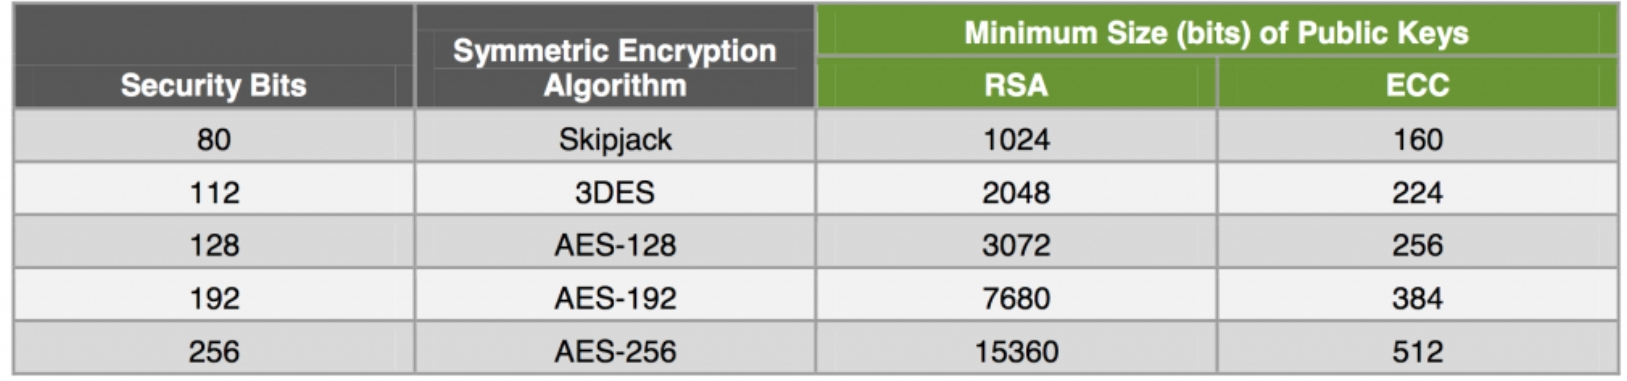
\includegraphics[width=0.8\textwidth]{image/section3/rsa.jpeg} 
    \caption[So sánh độ bảo mật giữa ECC và RSA]{So sánh độ bảo mật giữa ECC và RSA (\textbf{Nguồn:} \href{https://www.netburner.com/learn/comparing-rsa-and-ecc-encryption/}{NetBurner})}
    \label{}
\end{figure}

Có thể thấy rằng, mức bảo mật của khóa ECC-256 tương đương với khóa RSA-3072, trong khi kích thước khóa ECC nhỏ hơn hơn mười lần. Ưu điểm này mang lại lợi ích đáng kể trong các hệ thống nhúng (Embedded systems), nơi bộ nhớ, năng lượng và khả năng tính toán bị giới hạn.

\subsubsection{Đường cong NIST P-256}

Trong đề tài này, đường cong elliptic NIST P-256 (còn được gọi là \textit{secp256r1}) được sử dụng. Đường cong này được chuẩn hóa trong FIPS 186-4 \cite{fips186} và được xây dựng trên trường hữu hạn $\mathbb{F}_p$, với phương trình Weierstrass tổng quát:

\begin{equation}
y^2 \equiv x^3 + ax + b \pmod{p}
\end{equation}

\textbf{Các tham số của đường cong P-256} được xác định như sau:

\begin{align}
p &= 2^{256} - 2^{224} + 2^{192} + 2^{96} - 1 \\
a &= -3 \\
b &= \text{0x5AC635D8...} \quad \text{(hằng số 256 bit)}
\end{align}

Điểm sinh (base point) $G$ của đường cong có bậc (order) $n$ là một số nguyên tố lớn:

\begin{equation}
n = \text{0xFFFFFFFF00000000...} \quad \text{(số nguyên tố 256 bit)}
\end{equation}
\begin{figure}[H]
    \centering
    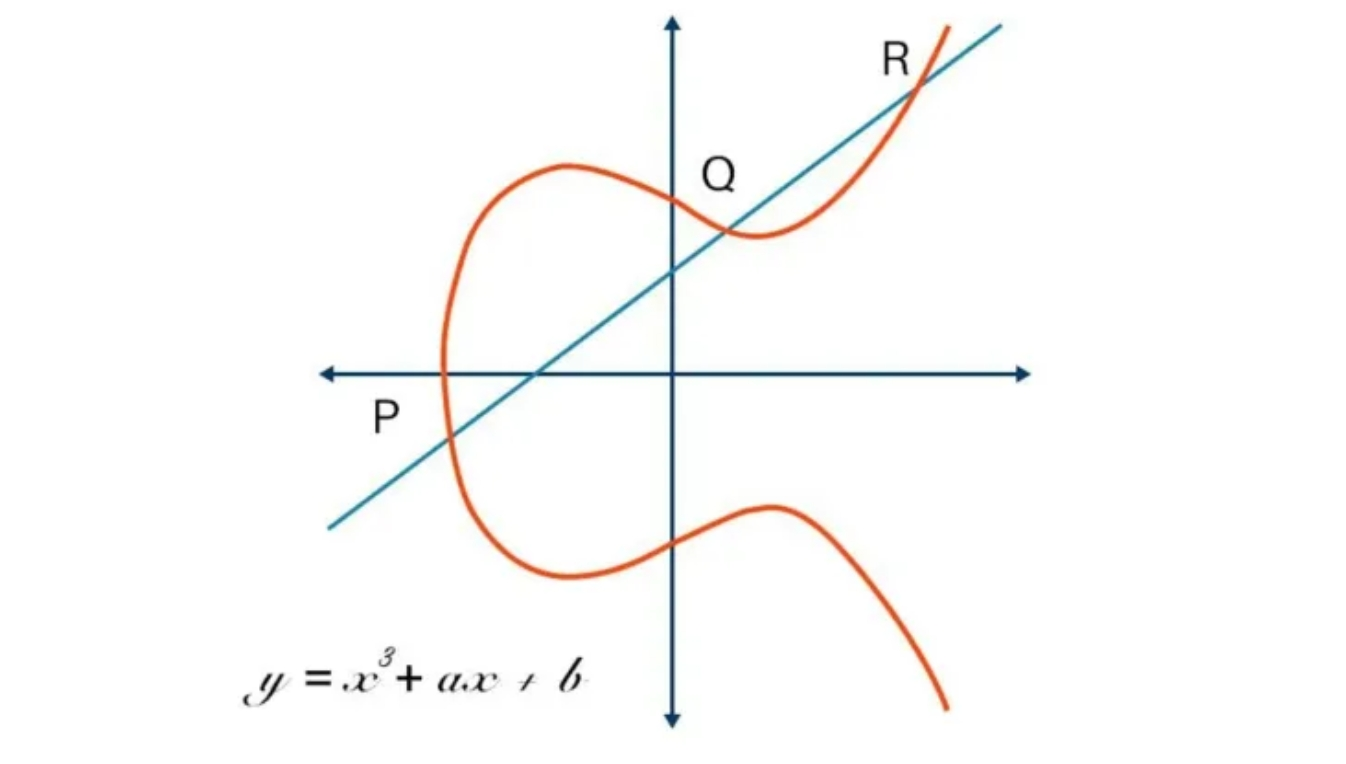
\includegraphics[width=0.8\textwidth]{image/section3/cry.jpeg} 
    \caption[Đồ thị đường cong Elliptic]{Đồ thị đường cong Elliptic (\textbf{Nguồn:} \href{https://blog.consultanubhav.com/elliptic-curve-cryptography-via-ope-5e91c059b817}{blog.consultanubhav.com})}
    \label{}
\end{figure}

\textbf{Các phép toán cơ bản trên đường cong}

\begin{itemize}
    \item \textbf{Cộng điểm (Point Addition):}  
    Cho hai điểm $P$ và $Q$ thuộc đường cong elliptic, phép cộng điểm tạo ra điểm thứ ba $R = P + Q$, được tính toán thông qua các phép toán đại số trên trường hữu hạn modulo $p$.
    
    \item \textbf{Nhân vô hướng (Scalar Multiplication):}  
    Phép nhân vô hướng là phép toán lặp phép cộng điểm nhiều lần:
    \begin{equation}
    Q = k \cdot P = \underbrace{P + P + \cdots + P}_{k \text{ lần}}
    \end{equation}
    Trong thực tế, phép toán này được thực hiện hiệu quả bằng thuật toán \textit{double-and-add}, với độ phức tạp tính toán là $O(\log k)$.
\end{itemize}

\textbf{Bài toán logarit rời rạc trên đường cong elliptic (ECDLP)}

Mức độ an toàn của ECC dựa trên độ khó của bài toán logarit rời rạc trên đường cong elliptic, được mô tả như sau:

\begin{quotation}
\textit{Cho hai điểm $P$ và $Q = k \cdot P$ trên đường cong elliptic, việc xác định giá trị vô hướng $k$ từ $P$ và $Q$ là một bài toán có độ phức tạp tính toán rất cao.}
\end{quotation}

Hiện nay, thuật toán hiệu quả nhất để giải bài toán ECDLP là thuật toán Pollard’s rho, với độ phức tạp xấp xỉ $O(\sqrt{n})$. Đối với đường cong P-256, độ phức tạp này tương đương khoảng $2^{128}$ phép toán, vượt quá khả năng tính toán của các hệ thống hiện tại.

\subsubsection{ECDH (Elliptic Curve Diffie-Hellman)}

ECDH (Elliptic Curve Diffie-Hellman) là giao thức trao đổi khóa dựa trên mật mã đường cong elliptic, cho phép hai bên thiết lập một \textbf{khóa bí mật chung} (shared secret) thông qua một kênh truyền không bảo mật. Giao thức này được chuẩn hóa trong NIST SP 800-56A Rev. 3 \cite{nist80056a} và được sử dụng rộng rãi trong các hệ thống bảo mật hiện đại.

\begin{figure}[htbp]
    \centering
    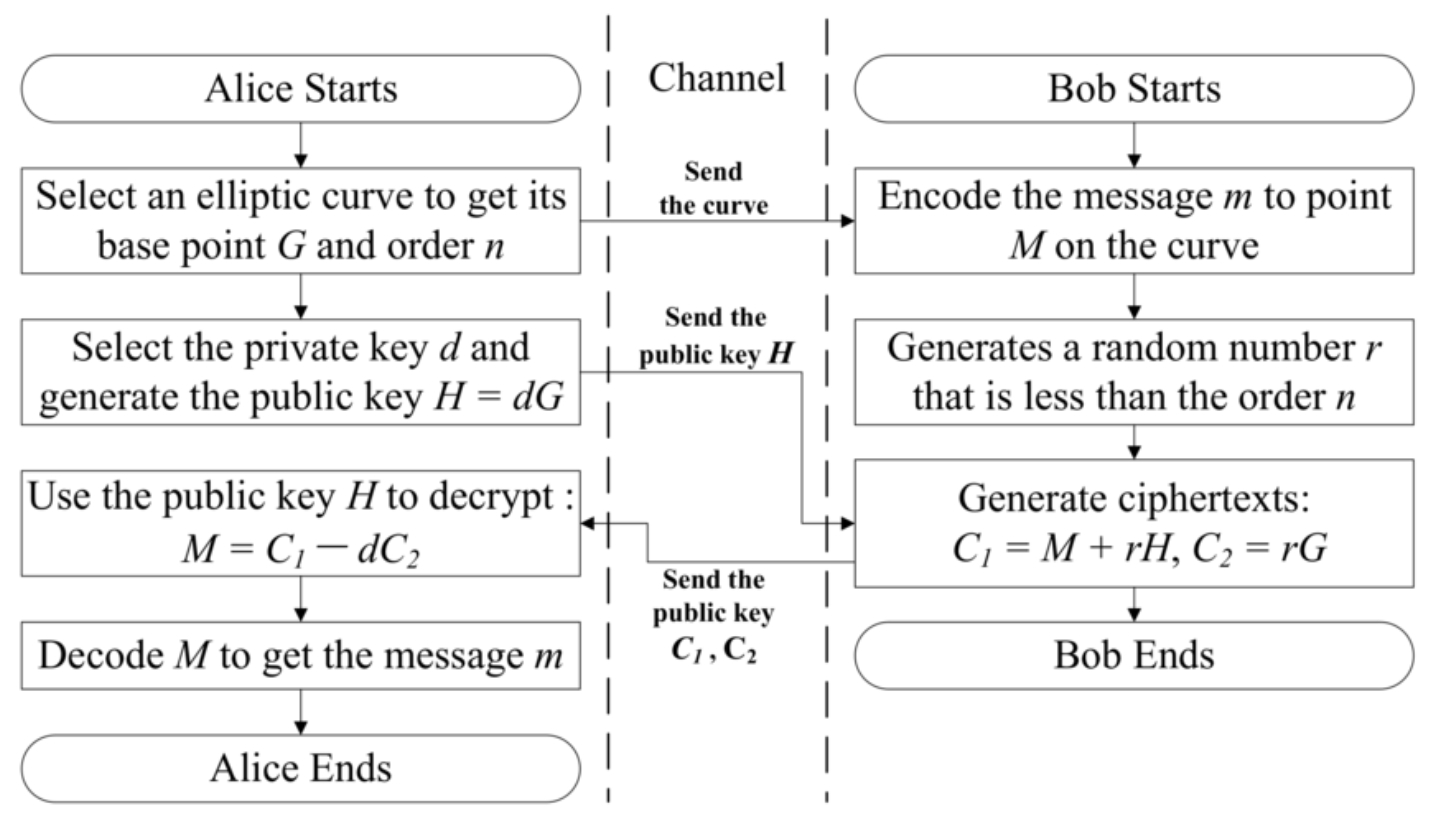
\includegraphics[width=0.8\textwidth]{image/section3/cry2.jpeg} 
    \caption[Sơ đồ giao thức ECDH]{Sơ đồ giao thức ECDH (\textbf{Nguồn:} \href{https://www.mdpi.com/2079-9292/11/18/2925}{MDPI})}
    \label{}
\end{figure}

\textbf{Quy trình giao thức ECDH}

Giả sử hai thực thể tham gia giao tiếp là Alice và Bob, quá trình thiết lập khóa được thực hiện như sau:

\begin{enumerate}
    \item \textbf{Alice tạo cặp khóa:}
    \begin{itemize}
        \item Khóa riêng: $d_A \in [1, n-1]$, được sinh ngẫu nhiên
        \item Khóa công khai: $Q_A = d_A \cdot G$
    \end{itemize}
    
    \item \textbf{Bob tạo cặp khóa:}
    \begin{itemize}
        \item Khóa riêng: $d_B \in [1, n-1]$, được sinh ngẫu nhiên
        \item Khóa công khai: $Q_B = d_B \cdot G$
    \end{itemize}
    
    \item \textbf{Trao đổi khóa công khai:}  
    Alice gửi khóa công khai $Q_A$ cho Bob; Bob gửi khóa công khai $Q_B$ cho Alice thông qua kênh truyền không bảo mật.
    
    \item \textbf{Tính toán khóa bí mật chung:}
    \begin{itemize}
        \item Alice tính:
        \[
        S = d_A \cdot Q_B = d_A \cdot (d_B \cdot G)
        \]
        \item Bob tính:
        \[
        S = d_B \cdot Q_A = d_B \cdot (d_A \cdot G)
        \]
    \end{itemize}
\end{enumerate}

Nhờ tính giao hoán của phép nhân vô hướng trên đường cong elliptic, cả hai bên thu được cùng một khóa bí mật chung:
\[
S = (d_A \cdot d_B) \cdot G
\]

\textbf{Các tính chất bảo mật}

\begin{itemize}
    \item \textbf{Tính bảo mật:}  
    Kẻ tấn công có thể quan sát được các khóa công khai $Q_A$ và $Q_B$, nhưng không thể suy ra khóa bí mật chung $S$ nếu không biết khóa riêng $d_A$ hoặc $d_B$. Điều này dựa trên độ khó của bài toán logarit rời rạc trên đường cong elliptic (ECDLP).
    
    \item \textbf{Forward Secrecy:}  
    Khi sử dụng \textbf{ephemeral keys} (cặp khóa tạm thời được tạo mới cho mỗi phiên), việc lộ khóa dài hạn không ảnh hưởng đến các khóa phiên đã được thiết lập trước đó.
\end{itemize}

\textbf{Ứng dụng trong đề tài}
\par\vspace{0.5em}
Trong đề tài này, ECDH được sử dụng ở \textbf{Phase B} của quá trình xác thực. Hai bên tạo cặp khóa ECDH tạm thời để thiết lập shared secret, sau đó sử dụng hàm dẫn xuất khóa HKDF để sinh ra các khóa phiên phục vụ cho mã hóa dữ liệu và kiểm tra toàn vẹn thông điệp (MAC).

\subsubsection{ECDSA (Elliptic Curve Digital Signature Algorithm)}

ECDSA (Elliptic Curve Digital Signature Algorithm) là thuật toán chữ ký số dựa trên mật mã đường cong elliptic (ECC), được chuẩn hóa trong tiêu chuẩn FIPS 186-4 \cite{fips186}. Thuật toán này cung cấp hai thuộc tính bảo mật quan trọng là \textbf{xác thực danh tính} (Authentication) và \textbf{tính không thể chối bỏ} (Non-repudiation).
\par\vspace{0.5em}
\textbf{Quy trình tạo chữ ký (Signing)}

Để tạo chữ ký số cho thông điệp $m$ bằng khóa riêng $d$, các bước được thực hiện như sau:

\begin{enumerate}
    \item Tính giá trị băm của thông điệp:
    \[
    e = \text{SHA-256}(m) \bmod n
    \]
    
    \item Sinh một số ngẫu nhiên bí mật (nonce):
    \[
    k \in [1, n-1]
    \]
    
    \item Tính điểm trên đường cong:
    \[
    R = k \cdot G = (x_R, y_R)
    \]
    
    \item Tính thành phần chữ ký thứ nhất:
    \[
    r = x_R \bmod n
    \]
    
    \item Tính thành phần chữ ký thứ hai:
    \[
    s = k^{-1} \cdot (e + r \cdot d) \bmod n
    \]
    
    \item Cặp giá trị $(r, s)$ tạo thành chữ ký số của thông điệp $m$.
\end{enumerate}

\textbf{Quy trình xác thực chữ ký (Verification)}

Để xác thực chữ ký $(r, s)$ của thông điệp $m$ bằng khóa công khai $Q$, các bước sau được thực hiện:

\begin{enumerate}
    \item Tính giá trị băm của thông điệp:
    \[
    e = \text{SHA-256}(m) \bmod n
    \]
    
    \item Tính nghịch đảo modulo của $s$:
    \[
    w = s^{-1} \bmod n
    \]
    
    \item Tính các hệ số trung gian:
    \[
    u_1 = e \cdot w \bmod n, \quad
    u_2 = r \cdot w \bmod n
    \]
    
    \item Tính điểm trên đường cong:
    \[
    P = u_1 \cdot G + u_2 \cdot Q = (x_P, y_P)
    \]
    
    \item Chữ ký được chấp nhận nếu:
    \[
    r \equiv x_P \bmod n
    \]
\end{enumerate}

\textbf{Các lưu ý bảo mật quan trọng}

\begin{itemize}
    \item \textbf{Tái sử dụng nonce:}  
    Việc sử dụng lại cùng một nonce $k$ cho nhiều chữ ký khác nhau là cực kỳ nguy hiểm, vì kẻ tấn công có thể khai thác để khôi phục khóa riêng $d$.
    
    \item \textbf{Bộ sinh số ngẫu nhiên:}  
    Nonce $k$ phải được sinh bằng bộ sinh số ngẫu nhiên an toàn về mặt mật mã (Cryptographically secure RNG) nhằm đảm bảo tính không thể dự đoán.
\end{itemize}

\textbf{Ứng dụng trong đề tài}
\par\vspace{0.5em}
ECDSA được sử dụng xuyên suốt trong hệ thống để đảm bảo xác thực danh tính và tính toàn vẹn dữ liệu:

\begin{itemize}
    \item \textbf{Phase A:} Điện thoại ký khóa công khai bằng khóa riêng định danh (identity private key), ESP32 xác thực chữ ký bằng khóa công khai đã được lưu trữ trước đó.
    
    \item \textbf{Phase B:} Điện thoại ký khóa công khai tạm thời (Ephemeral public key) và thông điệp thử thách (Challenge) nhằm chứng minh danh tính.
    
    \item Thư viện \textbf{mbedTLS} được sử dụng để triển khai ECDSA, đảm bảo  các phép toán mật mã được thực hiện an toàn.
\end{itemize}

%-----------------------------------------------------------------------

\subsection{Mã hóa đối xứng và xác thực thông điệp}

\subsubsection{AES-128-GCM – Advanced Encryption Standard}

AES là thuật toán mã hóa đối xứng được NIST lựa chọn làm chuẩn vào năm 2001 \cite{daemen2002design}.  
GCM là một chế độ mã hóa xác thực, kết hợp đồng thời chức năng mã hóa và xác thực thông điệp trong cùng một phép toán, được chuẩn hóa trong NIST SP 800-38D \cite{nist80038d}.
\begin{figure}[htbp]
    \centering
    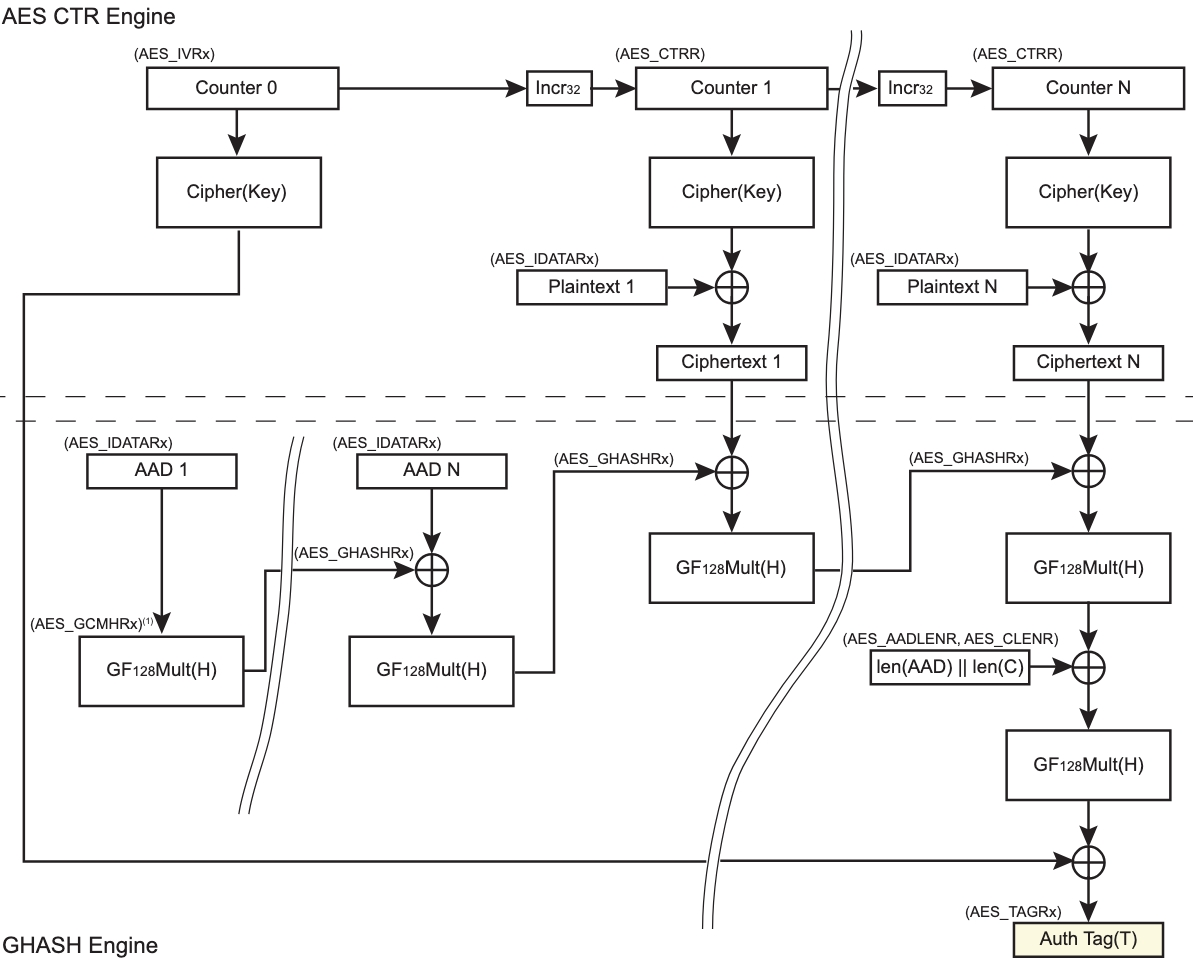
\includegraphics[width=0.8\textwidth]{image/section3/cry3.jpeg} 
    \caption[Cấu trúc AES-GCM]{Cấu trúc AES-GCM (\textbf{Nguồn:} \href{https://dl.acm.org/doi/10.1145/3766074}{dl.acm.org})}
    \label{}
\end{figure}

\textbf{Thông số kỹ thuật}

\begin{itemize}
    \item \textbf{Kích thước khóa:} 128 bit, đề tài sử dụng AES-128
    \item \textbf{Kích thước khối:} 128 bit
    \item \textbf{IV – Initialization Vector:} 96 bit, theo khuyến nghị của NIST
    \item \textbf{Authentication Tag:} 128 bit
\end{itemize}

\textbf{Thành phần của GCM}

\begin{enumerate}
    \item \textbf{Mã hóa theo chế độ CTR}

    Plaintext được XOR với keystream sinh ra từ quá trình mã hóa AES của giá trị counter:
    \begin{equation}
        C_i = P_i \oplus \text{AES}_K(\text{IV} \parallel \text{Counter}_i)
    \end{equation}

    \item \textbf{Xác thực bằng GHASH}

    Thuật toán GHASH sử dụng phép nhân trên trường Galois để tính toán authentication tag từ ciphertext và dữ liệu xác thực bổ sung:
    \begin{equation}
        T = \text{GHASH}_H(\text{AAD}, C)
    \end{equation}
\end{enumerate}

\textbf{Dữ liệu vào và dữ liệu ra}

\begin{itemize}
    \item \textbf{Dữ liệu vào:} Khóa $K$ 128 bit, IV 96 bit, Plaintext $P$, AAD (tùy chọn)
    \item \textbf{Dữ liệu ra:} Ciphertext $C$ và authentication tag $T$ 128 bit
\end{itemize}

\textbf{Các tính chất bảo mật}

\begin{itemize}
    \item \textbf{Confidentiality – Bảo mật:} Plaintext không thể được khôi phục nếu không có khóa bí mật
    \item \textbf{Authenticity – Xác thực:} Authentication tag cho phép phát hiện ciphertext bị giả mạo
    \item \textbf{Integrity – Toàn vẹn:} Bất kỳ thay đổi nào trong dữ liệu đều làm cho tag không hợp lệ
\end{itemize}

\textbf{Yêu cầu quan trọng}

\begin{itemize}
    \item \textbf{Tính duy nhất của IV:} IV phải là duy nhất cho mỗi lần mã hóa với cùng một khóa. Việc tái sử dụng IV gây ra lỗ hổng bảo mật nghiêm trọng \cite{joux2006authentication}.
    \item \textbf{Xác minh Authentication tag:} Authentication tag phải được kiểm tra trước khi sử dụng dữ liệu đã giải mã.
\end{itemize}

\textbf{Ứng dụng trong đề tài}
\par\vspace{0.5em}
Sau khi quá trình xác thực hoàn tất, AES-128-GCM được sử dụng để mã hóa dữ liệu trong phiên làm việc. IV(Initialization Vector) được sinh từ bộ sinh số ngẫu nhiên an toàn và kết hợp với Counter để đảm bảo tính duy nhất cho mỗi lần mã hóa.

\subsubsection{HMAC-SHA256 – Hash-based Message Authentication SHA-256}

HMAC là một cơ chế tạo mã xác thực thông điệp dựa trên hàm băm mật mã, được định nghĩa trong RFC 2104 \cite{rfc2104} và tiêu chuẩn hóa trong FIPS 198-1 \cite{fips198}.  
Thuật toán này kết hợp khóa bí mật với hàm băm để đảm bảo tính toàn vẹn và xác thực của dữ liệu trao đổi.
\par\vspace{0.5em}
\textbf{Công thức HMAC}

\begin{equation}
\text{HMAC}_K(m) = H\bigl((K \oplus \text{opad}) \parallel H((K \oplus \text{ipad}) \parallel m)\bigr)
\end{equation}

Trong đó:

\begin{itemize}
    \item $H$: Hàm băm mật mã, trong đề tài sử dụng SHA-256
    \item $K$: Khóa bí mật, độ dài 32 byte
    \item $\text{opad}$: Outer padding, giá trị 0x5c lặp lại theo độ dài khối
    \item $\text{ipad}$: Inner padding, giá trị 0x36 lặp lại theo độ dài khối
    \item $\parallel$: Phép nối chuỗi
\end{itemize}

\begin{figure}[H]
    \centering
    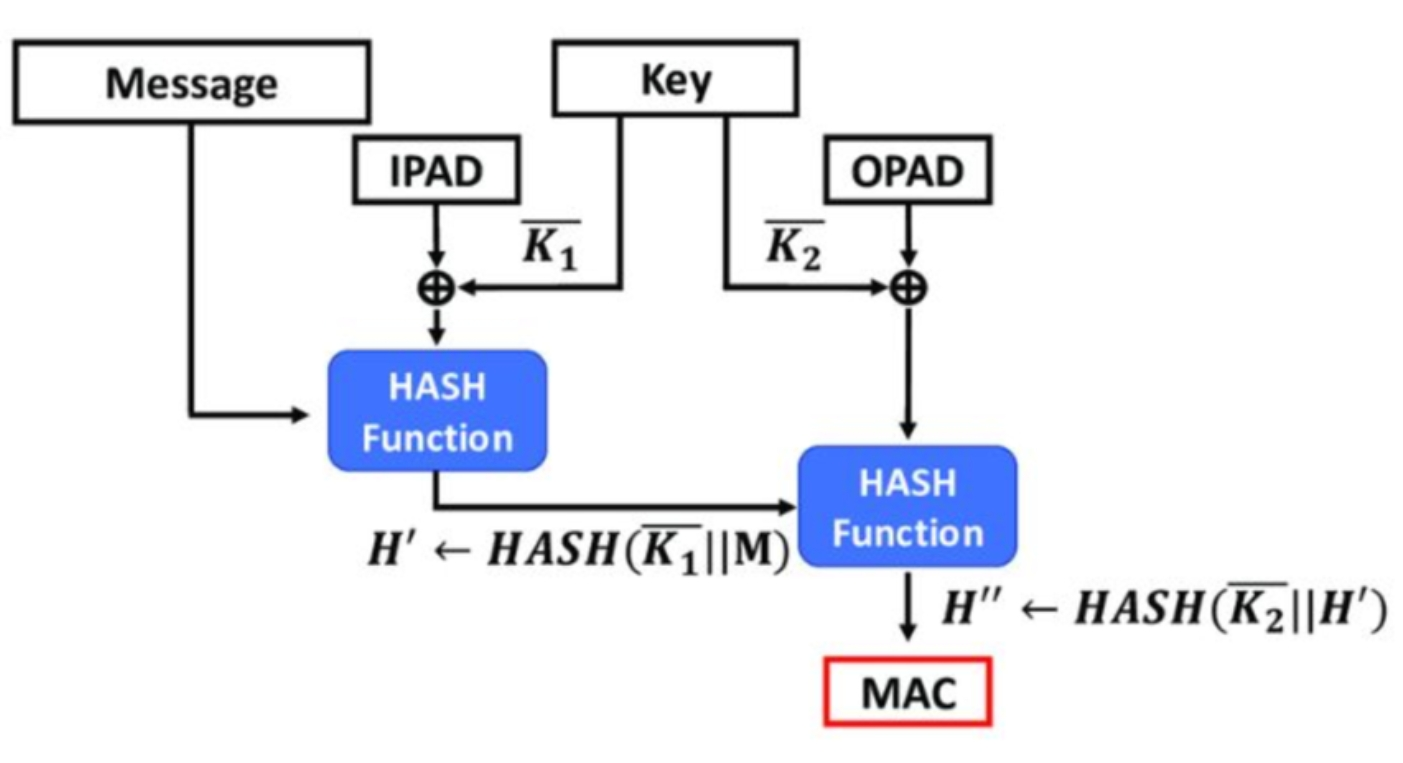
\includegraphics[width=0.8\textwidth]{image/section3/cry4.jpeg} 
    \caption[Cấu trúc HMAC]{Cấu trúc HMAC (\textbf{Nguồn:} \href{https://www.mdpi.com/2079-9292/9/11/1839}{MDPI})}
    \label{}
\end{figure}

\textbf{Thông số HMAC-SHA256 trong đề tài}

\begin{itemize}
    \item \textbf{Khóa đầu vào:} 32 byte, tương đương 256 bit
    \item \textbf{Giá trị đầu ra:} 32 byte, tương đương 256 bit
    \item \textbf{Mức độ bảo mật:} $2^{128}$, xét theo khả năng chống tấn công preimage đối với output rút gọn
\end{itemize}

\textbf{Các tính chất bảo mật}

\begin{itemize}
    \item \textbf{Unforgeability – Không thể giả mạo:} Không thể tạo ra HMAC hợp lệ nếu không biết khóa bí mật
    \item \textbf{Collision resistance – Chống va chạm:} Khó tìm hai thông điệp khác nhau cho cùng một giá trị HMAC
    \item \textbf{Key recovery resistance – Chống phục hồi khóa:} Không thể suy ra khóa bí mật từ các giá trị HMAC quan sát được
\end{itemize}

\textbf{Ứng dụng trong đề tài}

\begin{itemize}
    \item \textbf{Xác thực hai chiều:}  
    Điện thoại gửi $\text{HMAC}_{K_{c2s}}$ (Client confirm), thiết bị ESP32 xác minh và phản hồi bằng $\text{HMAC}_{K_{s2c}}$ (Server confirm)
    
    \item \textbf{Dẫn xuất khóa:}  
    Thuật toán HKDF sử dụng HMAC-SHA256 làm Primitive mật mã để sinh các Session keys
\end{itemize}


\subsubsection{HKDF – Hàm dẫn xuất khóa dựa trên HMAC}

HKDF là một hàm dẫn xuất khóa dựa trên HMAC, được định nghĩa trong RFC 5869 \cite{rfc5869}.  
Thuật toán này cho phép sinh ra nhiều khóa mật mã độc lập từ một Shared secret ban đầu, thường thu được từ các giao thức trao đổi khóa như ECDH.

\textbf{Cấu trúc của HKDF}

HKDF gồm hai giai đoạn liên tiếp: trích xuất và mở rộng.

\begin{enumerate}
    \item \textbf{Giai đoạn trích xuất – Extract Phase}
    
    Giai đoạn này chuyển Input keying material thành một khóa giả ngẫu nhiên có tính Entropy cao hơn, gọi là Pseudorandom key (PRK):
    \begin{equation}
    \text{PRK} = \text{HMAC}(\text{salt}, \text{IKM})
    \end{equation}
        \begin{figure}[H]
        \centering
        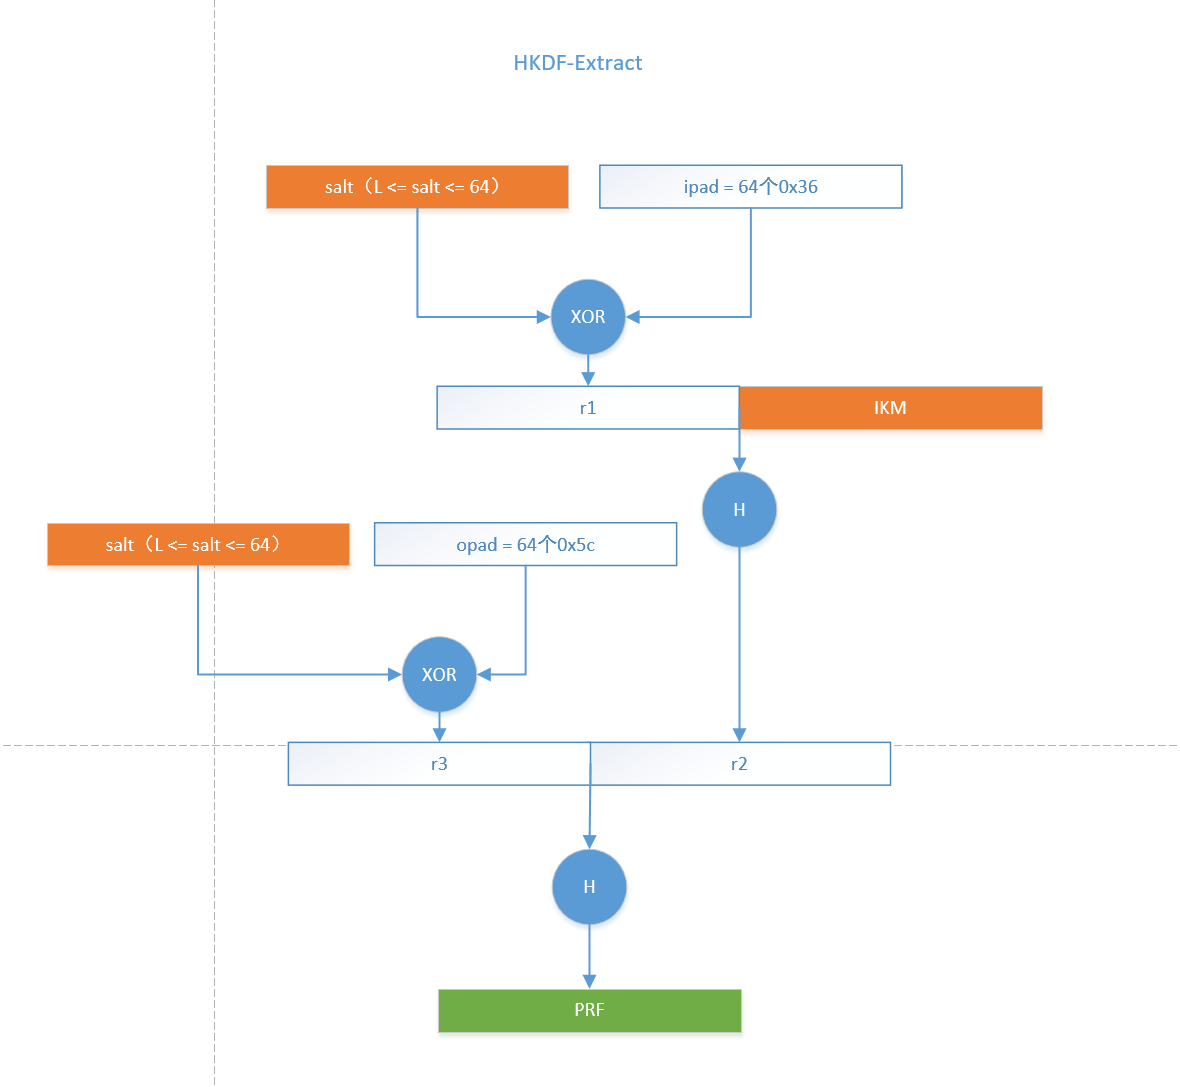
\includegraphics[width=0.5\textwidth]{image/section3/cry6.png} 
        \caption[Cấu trúc HKDF Extract]{Cấu trúc HKDF Extract (\textbf{Nguồn:} \href{https://suntus.github.io/2019/05/09/HKDF\%E7\%AE\%97\%E6\%B3\%95/}{HKDF - Morning~Sun})}
        \label{fig: hkdf_extract}
        \end{figure}
    \item \textbf{Giai đoạn mở rộng – Expand Phase}
    
    PRK được sử dụng để sinh ra một hoặc nhiều khóa đầu ra thông qua thông tin ngữ cảnh:
    \begin{align}
    T(0) &= \text{chuỗi rỗng} \\
    T(i) &= \text{HMAC}(\text{PRK}, T(i-1) \parallel \text{info} \parallel i)
    \end{align}
\end{enumerate}

\begin{figure}[H]
    \centering
    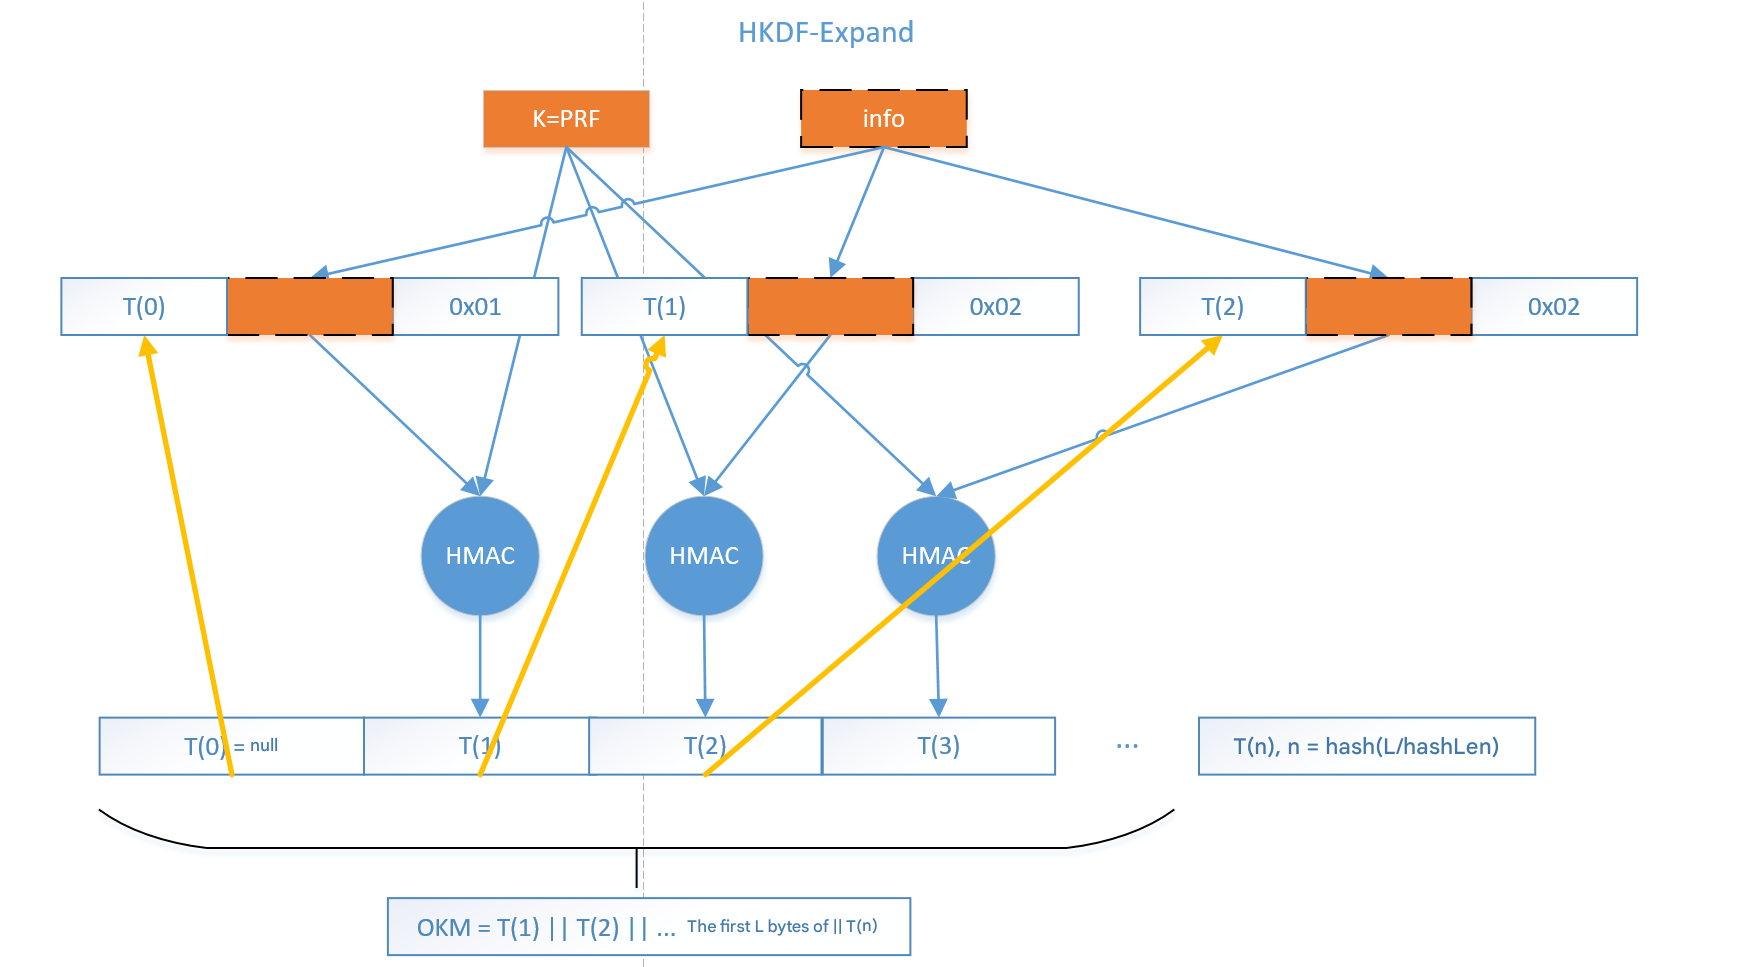
\includegraphics[width=0.8\textwidth]{image/section3/cry7.png} 
    \caption[Cấu trúc HKDF Expand]{Cấu trúc HKDF Expand (\textbf{Nguồn:} \href{https://suntus.github.io/2019/05/09/HKDF\%E7\%AE\%97\%E6\%B3\%95/}{HKDF - Morning~Sun})}
    \label{fig: hkdf_expand}
\end{figure}

\textbf{Các tham số của HKDF}

\begin{itemize}
    \item \textbf{IKM – Input Keying Material:} Dữ liệu đầu vào cho HKDF, trong đề tài là shared secret thu được từ ECDH, độ dài 32 byte
    \item \textbf{Salt:} Giá trị ngẫu nhiên tùy chọn dùng trong giai đoạn extract, không được sử dụng trong đề tài
    \item \textbf{Info:} Thông tin ngữ cảnh để ràng buộc khóa với phiên và ứng dụng cụ thể
    \item \textbf{L:} Độ dài khóa đầu ra mong muốn
\end{itemize}

\textbf{Tính chất bảo mật}

\begin{itemize}
    \item \textbf{Key independence – Tính độc lập của khóa:}  
    Các khóa được dẫn xuất với giá trị Info khác nhau là độc lập về mặt mật mã
    
    \item \textbf{Forward compatibility – Khả năng mở rộng về sau:}  
    Có thể sinh thêm các khóa mới mà không ảnh hưởng đến các khóa đã tồn tại
\end{itemize}

\textbf{Ứng dụng trong đề tài}

Từ Shared secret thu được trong quá trình trao đổi khóa ECDH, đề tài dẫn xuất các khóa phiên (Session Keys) nhằm mã hóa kênh truyền BLE và liên kết trực tiếp với phiên đo khoảng cách UWB:

\begin{lstlisting}[language=C++]
       // 1. Encryption Key
       info_enc = "SmartCarv1|ENC" || ecuPubKey || phonePubKey
       K_enc = HKDF-SHA256(sharedSecret, salt="", info_enc, L=32)

       // 2. MAC Key
       info_mac = "SmartCarv1|MAC" || ecuPubKey || phonePubKey
       K_mac = HKDF-SHA256(sharedSecret, salt="", info_mac, L=32)
       
       // 3. URSK - UWB Ranging Session Key
       info_uwb = "SmartCarv1|URSK" || ecuPubKey || phonePubKey
       K_ursk = HKDF-SHA256(sharedSecret, salt="", info_uwb, L=32)
\end{lstlisting}

Điểm đột phá trong giao thức bảo mật của đề tài (bám sát CCC Release 3) là việc khóa \texttt{K\_ursk} được sinh ra từ chính phiên giao tiếp BLE. Khóa này sau đó được nạp vào vi mạch UWB để mã hóa chuỗi STS (Scrambled Timestamp Sequence). Sự ràng buộc mật mã này đảm bảo rằng: Ngay cả khi kẻ tấn công can thiệp được vào sóng UWB, chúng cũng không thể giải mã hoặc đánh lừa được hệ thống đo khoảng cách vì không sở hữu khóa phiên bắt nguồn từ giao dịch BLE.
%-----------------------------------------------------------------------

\subsection{Tuân thủ chuẩn quốc tế}

Giao thức bảo mật của đề tài được thiết kế tuân thủ các chuẩn sau:

\begin{table}[h]
\centering
\label{tab:crypto_standards}
\begin{tabular}{|l|l|p{6cm}|}
\hline
\textbf{Chuẩn} & \textbf{Thuật toán} & \textbf{Mô tả} \\
\hline
NIST SP 800-56A Rev. 3 & ECDH & Key agreement với P-256 curve \\
\hline
FIPS 186-4 & ECDSA & Digital signature với P-256 \\
\hline
NIST SP 800-38D & AES-GCM & Authenticated encryption \\
\hline
FIPS 198-1 & HMAC-SHA256 & Message authentication \\
\hline
RFC 5869 & HKDF & Key derivation function \\
\hline
ISO/IEC 7816-4 & APDU & NFC communication protocol \\
\hline
\end{tabular}
\caption{Chuẩn mật mã được áp dụng}
\end{table}

Việc tuân thủ các chuẩn quốc tế đảm bảo:
\begin{itemize}
    \item Tính tương thích (Interoperability)
    \item Độ tin cậy về bảo mật (Security assurance)
    \item Khả năng chấp nhận trong công nghiệp (Industry acceptance)
\end{itemize}


\section{Công nghệ phát triển ứng dụng di động}

Ứng dụng di động (Smart Car) trong hệ thống được phát triển dựa trên Flutter Framework kết hợp với hệ sinh thái Firebase. Trong kiến trúc Hybrid Cloud của đề tài, Flutter không chỉ đảm nhiệm việc xây dựng giao diện người dùng mà còn đóng vai trò là Gateway trung gian, quản lý máy trạng thái (FSM) của khóa kỹ thuật số theo chuẩn CCC, xử lý các luồng dữ liệu bất đồng bộ từ phần cứng (BLE, UWB, NFC) và đồng bộ hóa với dịch vụ Cloud.

\subsection{Flutter Framework và Quản lý trạng thái}

Flutter là framework mã nguồn mở do Google phát triển, cho phép xây dựng ứng dụng đa nền tảng từ một codebase duy nhất sử dụng ngôn ngữ Dart. Đặc trưng nổi bật của Flutter là cơ chế biên dịch Ahead-of-Time (AOT), chuyển mã Dart trực tiếp sang mã máy ARM hoặc x86. Thay vì sử dụng JavaScript bridge hoặc WebView như các framework hybrid truyền thống, Flutter tự render toàn bộ giao diện thông qua đồ họa Skia/Impeller, giúp ứng dụng đạt hiệu năng cao và thời gian phản hồi thấp, đáp ứng tốt yêu cầu xử lý thời gian thực của hệ thống Smart Key.

\begin{figure}[H]
    \centering
    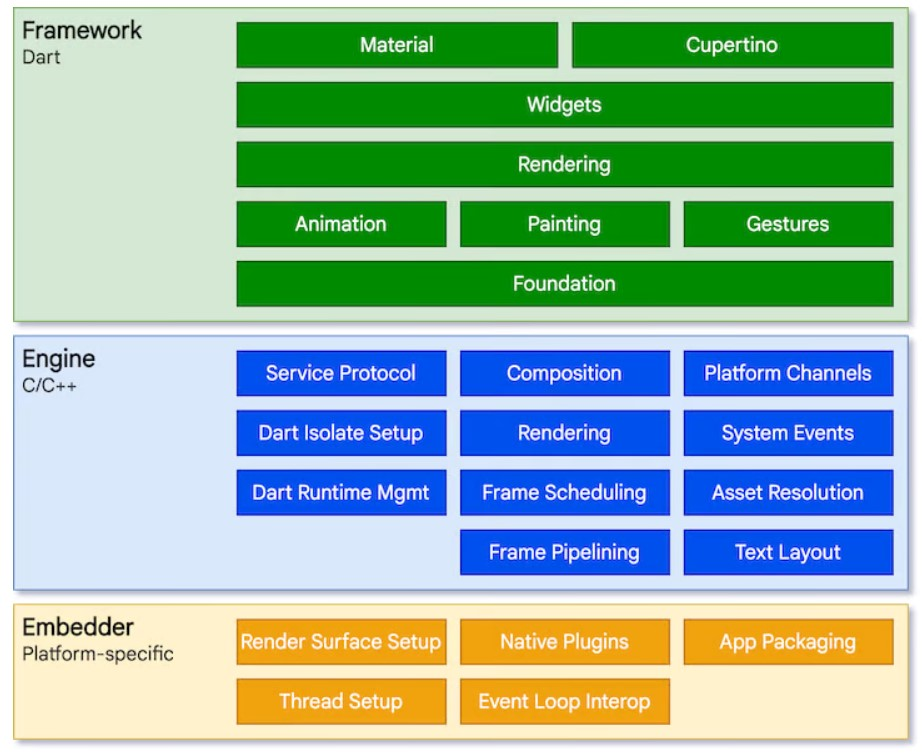
\includegraphics[width=0.8\textwidth]{image/section3/flu.jpg}
    \caption[Kiến trúc tổng thể của Flutter Framework]{Kiến trúc tổng thể của Flutter Framework (\textbf{Nguồn:} \href{https://bizflycloud.vn/tin-tuc/flutter-la-gi-tim-hieu-tinh-nang-noi-troi-cua-nen-tang-lap-trinh-flutter-20220623155918472.htm}{BizFlyCloud})}
    \label{fig: flutter_architecture}
\end{figure}

Kiến trúc của Flutter được tổ chức thành bốn tầng chính, hỗ trợ đắc lực cho việc phát triển ứng dụng giao tiếp phần cứng sâu:
\begin{itemize}
    \item \textbf{Application Layer:} Chứa mã Dart do lập trình viên xây dựng. Để quản lý sự phức tạp của các sự kiện phần cứng và luồng xác thực đa bước, ứng dụng áp dụng kiến trúc \textbf{BLoC (Business Logic Component)}. Mô hình này tách biệt hoàn toàn giao diện (UI) khỏi logic nghiệp vụ, giúp xử lý mượt mà các luồng dữ liệu (Streams) liên tục từ BLE, UWB và Firebase.
    \item \textbf{Framework Layer:} Cung cấp hệ thống widget nền tảng (Material, Cupertino), quản lý animation và pipeline render giao diện.
    \item \textbf{Engine Layer:} Core engine viết bằng C++, bao gồm đồ họa, Dart runtime và quản lý luồng (thread management).
    \item \textbf{Embedder Layer:} Đóng vai trò cầu nối giữa Flutter engine và hệ điều hành cụ thể (Android/iOS).
\end{itemize}

\textbf{Tương tác phần cứng qua Platform Channels:} \\
Một trong những lý do cốt lõi để chọn Flutter cho đề tài này là cơ chế Platform Channels. Cơ chế này cho phép luồng mã Dart giao tiếp trực tiếp và hai chiều với mã Native (Java/Kotlin trên Android, Swift trên iOS) thông qua \textit{MethodChannel} và \textit{EventChannel}. 

Tính năng này mang tính quyết định trong việc hiện thực hóa các chức năng bậc cao của chuẩn CCC Release 3, bao gồm:
\begin{itemize}
    \item Giao tiếp trực tiếp với các API Native của hệ điều hành để cấu hình \textbf{phiên UWB (UWB Session)} phục vụ đo khoảng cách an toàn (Secure Ranging).
    \item Thiết lập và duy trì \textbf{Background Services} cho phép ứng dụng quét BLE ngầm, phục vụ tính năng Auto-Unlock (Fast Authentication) mà không cần mở ứng dụng.
    \item Kích hoạt chế độ mô phỏng thẻ \textbf{NFC HCE (Host Card Emulation)}, biến điện thoại thành thẻ từ để thực hiện giao dịch Phase 0 dự phòng.
\end{itemize}

\subsection{Firebase Backend-as-a-Service}
Firebase là nền tảng Backend-as-a-Service (BaaS) do Google cung cấp, bao gồm tập hợp các dịch vụ backend được quản lý sẵn như xác thực người dùng, cơ sở dữ liệu thời gian thực, lưu trữ và điện toán phi máy chủ (serverless) \cite{firebase_docs}. Nền tảng này cho phép ứng dụng client giao tiếp trực tiếp với backend thông qua các SDK tích hợp sẵn hoặc REST API, giúp giảm thiểu tối đa sự phức tạp trong việc triển khai, duy trì và mở rộng hệ thống máy chủ vật lý.
\begin{figure}[H]
    \centering
    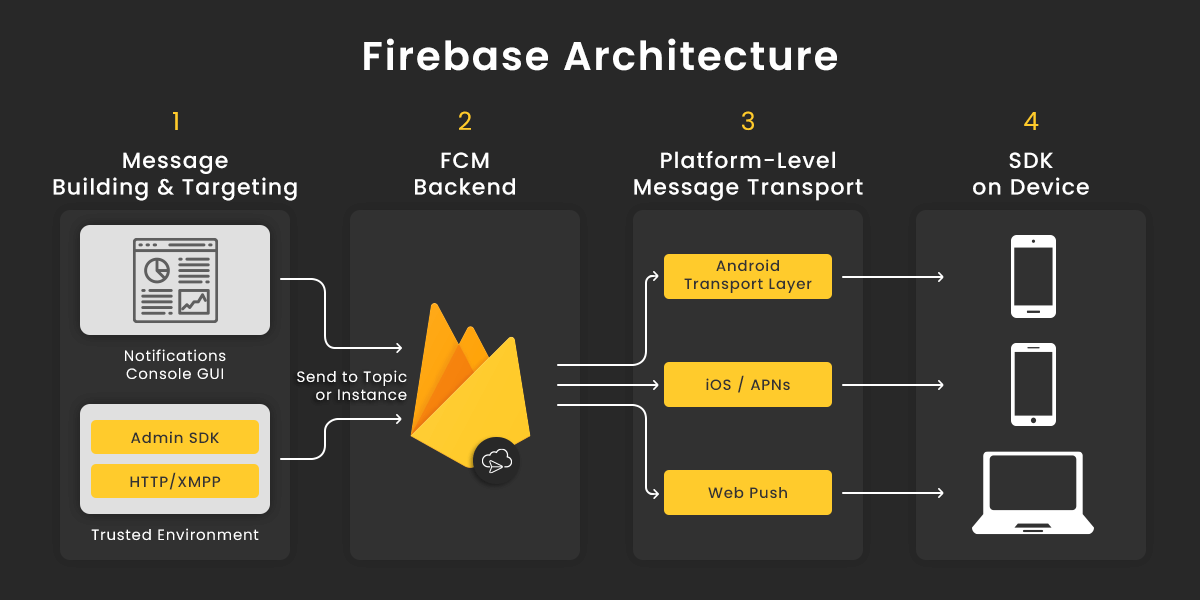
\includegraphics[width=0.85\textwidth]{image/section3/fire.png}
    \caption[Kiến trúc các dịch vụ Firebase trong hệ thống]{Kiến trúc các dịch vụ Firebase trong hệ thống (\textbf{Nguồn:} \href{https://bumblebeedev.hashnode.dev/2024-guide-to-creating-scalable-backend-apis-with-firebase}{BumblebeeDev})}
    \label{fig:firebase_architecture}
\end{figure}
\begin{itemize}
    \item \textbf{Firebase Authentication (Xác thực và định danh):}\\
    Trong hệ thống, Firebase Authentication được sử dụng để quản lý quá trình xác thực và định danh người dùng. Dịch vụ này hỗ trợ đa dạng các phương thức đăng nhập và tự động quản lý toàn bộ vòng đời của phiên làm việc (session), bao gồm việc phát hành, mã hóa và làm mới token (Token refresh). Firebase Authentication tuân thủ các tiêu chuẩn bảo mật mạng toàn cầu như OAuth 2.0 và OpenID Connect, đảm bảo an toàn tuyệt đối cho thông tin định danh trước các rủi ro đánh cắp phiên (Session Hijacking) hoặc nghe lén (Eavesdropping).

    \item \textbf{Cloud Firestore và Realtime Database (Lưu trữ và đồng bộ thời gian thực):}\\
    Cloud Firestore là cơ sở dữ liệu NoSQL dạng tài liệu (Document-based) của Firebase, được tối ưu hóa cho khả năng đồng bộ dữ liệu thời gian thực (Real-time synchronization) giữa các client. Dữ liệu được tổ chức theo mô hình phân cấp Collection và Document, cho phép linh hoạt lưu trữ các cấu trúc dữ liệu phức tạp. Cơ sở dữ liệu này hỗ trợ cơ chế cache dữ liệu ngoại tuyến (offline caching), tự động giải quyết xung đột và đồng bộ trạng thái khi kết nối mạng được khôi phục. 
    
    Bên cạnh đó, hệ thống phân quyền của Firestore được kiểm soát chặt chẽ thông qua Security Rules thực thi tại phía server. Cơ chế này đảm bảo chỉ những thiết bị hoặc người dùng có token hợp lệ, được cấp quyền tương ứng mới có thể thực hiện các thao tác truy xuất (Read) hoặc thay đổi (Write) dữ liệu, tạo ra một lớp phòng thủ độc lập hoàn toàn với client.

    \item \textbf{Firebase Cloud Messaging (FCM) - Giao thức truyền tin nhắn:}\\
    Firebase Cloud Messaging (FCM) là dịch vụ nhắn tin đa nền tảng, cung cấp cơ sở hạ tầng mạng định tuyến thông điệp có độ trễ thấp từ máy chủ đến thiết bị người dùng (Client). Trong các hệ thống yêu cầu tính thời gian thực cao, FCM đóng vai trò là kênh giao tiếp Push Notification tin cậy. Dịch vụ này sử dụng kiến trúc Pub/Sub (Publish/Subscribe), cho phép gửi cảnh báo ngay lập tức để đánh thức các ứng dụng đang chạy ngầm (background) hoặc đã tắt hoàn toàn (terminated), đảm bảo người dùng nhận được các thông báo an ninh quan trọng ngay tại thời điểm sự kiện phát sinh.

    \item \textbf{Khả năng tích hợp IoT và Event-Driven Architecture:}\\
    Mặc dù được thiết kế chủ yếu cho hệ sinh thái Web và Mobile, Firebase cung cấp hệ thống REST API mạnh mẽ, cho phép các thiết bị nhúng với tài nguyên phần cứng giới hạn (như vi điều khiển) giao tiếp trực tiếp qua giao thức HTTPS. Các thiết bị biên (Edge devices) có thể đẩy trực tiếp dữ liệu nhật ký hoạt động (Access Logs) hoặc trạng thái phần cứng lên cơ sở dữ liệu đám mây. 
    
    Khi kết hợp với \textbf{Firebase Cloud Functions} – môi trường thực thi mã backend phi máy chủ (Serverless), hệ thống có thể vận hành theo kiến trúc hướng sự kiện (Event-driven). Bất kỳ một luồng dữ liệu mới nào được ghi vào cơ sở dữ liệu từ thiết bị IoT cũng có thể trở thành một trigger (bộ kích hoạt), tự động gọi các hàm tính toán logic trên server hoặc giao tiếp với các hệ thống phân tích Trí tuệ nhân tạo (AI) bên thứ ba để phát hiện sự kiện bất thường mà không làm tiêu tốn tài nguyên của thiết bị biên.
\end{itemize}


Trong hệ thống, \textbf{Firebase Authentication} đảm nhiệm việc xác thực và định danh người dùng. Dịch vụ này tự động quản lý vòng đời phiên làm việc (cấp phát và làm mới token) dựa trên các tiêu chuẩn bảo mật nền tảng như OAuth 2.0 và OpenID Connect.

Bên cạnh đó, \textbf{Cloud Firestore} được sử dụng làm cơ sở dữ liệu NoSQL dạng tài liệu (document-based) nhằm lưu trữ linh hoạt và đồng bộ dữ liệu theo thời gian thực. Firestore hỗ trợ hoạt động ngoại tuyến (offline cache) và tích hợp cơ chế \textit{Security Rules} thực thi tại server, đảm bảo chỉ những client đã xác thực và có quyền hợp lệ mới được phép truy xuất hoặc thay đổi dữ liệu.




%----------------------------------------------------------------------------------------------



\section{Mô hình học sâu LSTM cho nhận diện hành vi}

Trong bài toán nhận diện hành vi người dùng dựa trên dữ liệu từ cảm biến UWB, các tín hiệu (khoảng cách, vận tốc, thặng dư) không tồn tại độc lập mà có sự phụ thuộc chặt chẽ vào thời gian. Các mạng nơ-ron truyền thống (Feed-forward Neural Network) không thể xử lý loại dữ liệu chuỗi này do thiếu cơ chế ghi nhớ các trạng thái quá khứ. Mạng nơ-ron hồi quy (RNN) ra đời để giải quyết vấn đề này, tuy nhiên RNN gặp phải hiện tượng "biến mất gradient" (Vanishing Gradient) khi xử lý các chuỗi dài, khiến mô hình không thể học được các phụ thuộc xa (long-term dependencies).Kiến trúc LSTM, được giới thiệu bởi Hochreiter \& Schmidhuber (1997), là một biến thể đặc biệt của RNN được thiết kế để khắc phục nhược điểm trên. Trong hệ thống Smart Car Access của đề tài, LSTM đóng vai trò nhận diện các "hình thái" chuyển động (như việc tiến lại gần xe hoặc các dao động bất thường của tấn công tiếp sóng) thông qua một cửa sổ thời gian (sliding window).

\subsection{Kiến trúc và cơ chế hoạt động của LSTM}Điểm khác biệt cốt lõi của LSTM là sự xuất hiện của Trạng thái tế bào (Cell State) — đóng vai trò như một "băng chuyền" thông tin chạy xuyên suốt chuỗi — và các Cổng (Gates) để điều tiết việc thêm hoặc bớt thông tin vào trạng thái đó.Mỗi tế bào LSTM tại thời điểm $t$ nhận đầu vào là dữ liệu hiện tại $x_t$, trạng thái ẩn của thời điểm trước $h_{t-1}$ và trạng thái tế bào trước $C_{t-1}$. Quá trình xử lý được thực hiện qua các bước toán học sau:
\begin{enumerate}
\item \textbf{Cổng quên (Forget Gate):} Quyết định thông tin nào từ trạng thái tế bào cũ sẽ bị loại bỏ.
\begin{equation}
    f_t = \sigma(W_f \cdot [h_{t-1}, x_t] + b_f)
\end{equation}
Trong đó $\sigma$ là hàm kích hoạt Sigmoid, đầu ra $f_t \in [0, 1]$. Nếu $f_t \approx 0$, thông tin cũ sẽ bị xóa bỏ.

\item \textbf{Cổng đầu vào (Input Gate):} Quyết định thông tin mới nào sẽ được lưu trữ vào trạng thái tế bào.
\begin{equation}
    i_t = \sigma(W_i \cdot [h_{t-1}, x_t] + b_i)
\end{equation}
Đồng thời, một lớp $\tanh$ tạo ra một vector ứng viên $\tilde{C}_t$ chứa các giá trị mới có thể thêm vào:
\begin{equation}
    \tilde{C}_t = \tanh(W_C \cdot [h_{t-1}, x_t] + b_C)
\end{equation}

\item \textbf{Cập nhật trạng thái tế bào (Cell State Update):} Kết hợp kết quả từ cổng quên và cổng đầu vào để tạo trạng thái mới $C_t$:
\begin{equation}
    C_t = f_t * C_{t-1} + i_t * \tilde{C}_t
\end{equation}

\item \textbf{Cổng đầu ra (Output Gate):} Quyết định giá trị của trạng thái ẩn $h_t$ dựa trên trạng thái tế bào đã được lọc qua hàm $\tanh$:
\begin{equation}
    o_t = \sigma(W_o \cdot [h_{t-1}, x_t] + b_o)
\end{equation}
\begin{equation}
    h_t = o_t * \tanh(C_t)
\end{equation}
\end{enumerate}

\subsection{Ứng dụng LSTM trong hệ thống định vị UWB}Trong phạm vi đề tài, mô hình LSTM được thiết kế để xử lý dữ liệu từ cửa sổ trượt có kích thước $T$ (thời điểm thực tế sử dụng $T=25$ frames).Vector đầu vào tại mỗi bước thời gian $t$ là $x_t = [d_t, r_t, v_t]^T$, trong đó:

\begin{itemize}
\item $d_t$: Khoảng cách đã qua bộ lọc Kalman.
\item $r_t$: Giá trị thặng dư (Residual) đại diện cho nhiễu vật lý.
\item $v_t$: Vận tốc tức thời của đối tượng.
\end{itemize}


Dữ liệu sau khi đi qua các lớp LSTM sẽ được đưa vào lớp kết nối đầy đủ và cuối cùng là hàm Softmax để phân loại xác suất cho 3 nhãn hành vi:

\begin{equation}P(y=k|X) = \frac{e^{z_k}}{\sum_{j=1}^{K} e^{z_j}}\end{equation}

với $K=3$ tương ứng với các nhãn: Walk (0), Loiter (1), và Relay Attack (2). Việc sử dụng LSTM giúp hệ thống không chỉ phản ứng với khoảng cách tức thời mà còn có khả năng nhận diện các "kịch bản" di chuyển phức tạp, nâng cao tính an toàn cho giải pháp Smart Car Access.